% ===================================================
% CHAPITRE 20 — L'ÉGLISE D'OUROUX
% Pages imprimées 181-230 — vues 184-233
% ===================================================
\chapter{L'église d'Ouroux}

% --- Page imprimée 181 — vue 184
\begin{center}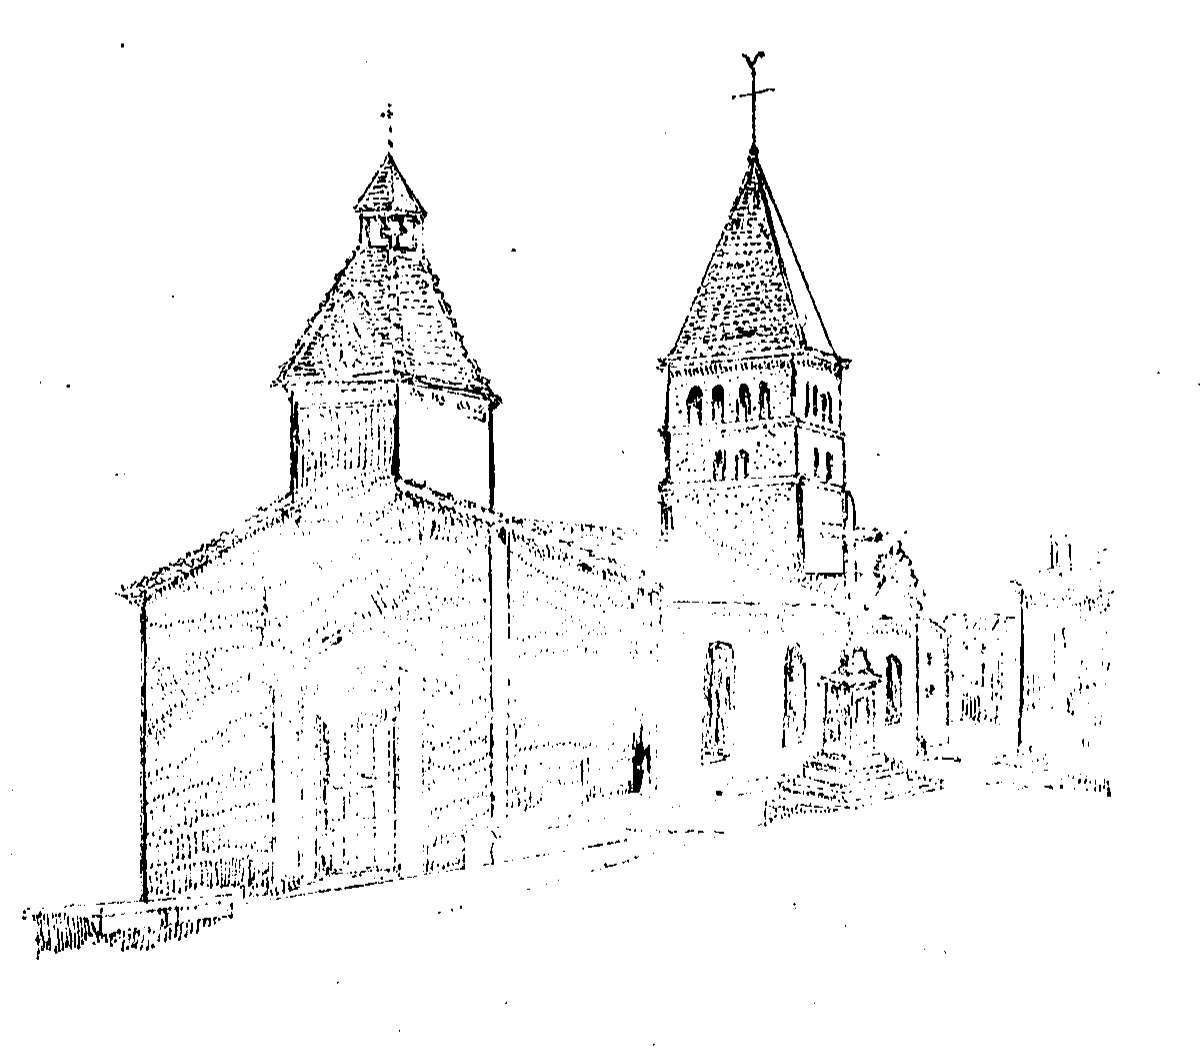
\includegraphics[width=0.62\textwidth]{Illustrations/illus-eglise-saint-antoine.jpg}\par
\textit{Église Saint-Antoine d'Ouroux (avec son ancien clocheton)}\end{center}

% --- Page imprimée 182 — vue 185
L'architecture seule peut nous permettre de déterminer approximativement l'époque à laquelle l'église d'Ouroux fut construite. Ses fenêtres à plein cintre, ses voûtes en ogive, nous rappellent la période romano-byzantine de transition, période qui s'étend du commencement du XIIème siècle au commencement du XIIIème. Elle est plutôt néanmoins de la fin du XIIème siècle, car dans la première moitié, les voûtes en ogive sont fort peu régulières : ou bien elles s'éloignent du plein cintre, ou bien elles sont très aiguës. Celles de notre chœur, au contraire, sont parfaitement régulières.

L'église actuelle a certainement remplacé une église plus ancienne puisque Ouroux était depuis longtemps paroisse et comme cela avait lieu fréquemment, on a pu faire servir aux constructions nouvelles, dans une certaine mesure, les fondations anciennes. Il n'en subsiste néanmoins aucune trace à cette heure. Il est possible toutefois que la tête de moine encastrée dans le mur extérieur de l'abside provienne de cette ancienne église. Cette tête en pierre du pays et grossièrement sculptée offre bien l'aspect d'une tête de religieux avec sa couronne monacale et sa physionomie austère. Elle a dû servir de support, car la partie supérieure est sensiblement aplatie. Sa position irrégulière entre deux contreforts ne permet pas de supposer qu'elle a été placée là comme ornement. On sait que dans les siècles qui précédèrent l'époque qui nous occupe on employait pour recevoir les arcs des modillons ou pierres saillantes en forme de consoles que l'on sculptait diversement. L'exécution plus originale de celui-ci aurait déterminé les ouvriers à le conserver.

Comme architecture, l'église d'Ouroux appartient au style Gourguignon employé exclusivement à tout autre dans nos paroisses voisines du célèbre monastère de Cluny.

Dans le principe et jusque vers le milieu du XVème siècle le chœur avait la forme actuelle. Au centre du transept, une coupole octogonale reposant par ses quatre pans plus développés sur quatre arcs en ogive

% --- Page imprimée 183 — vue 186
Les angles sont remplis par les pendentifs qui servent eux-mêmes de supports aux quatre pans plus petits de la coupole.

Les deux bras du transept sont surmontés d'une voûte ogivale sans ornement.

L'abside semi-circulaire, soutenue extérieurement par cinq contreforts très simples avait trois baies entourées à l'intérieur d'une archivolte décorée de moulures et reposant sur des pilastres ornés eux-mêmes de cannelures et autres ornements de la période romane. Une corniche très simple ornait l'abside et les gros piliers du chœur à la naissance de l'ogive. À l'entrée du chœur, deux colonnes à demi engagées dans les piliers et surmontées d'un chapiteau à feuillages supportaient l'arc doubleau de l'arcade qui sépare la nef du chœur.

Deux baies étroites comme celles de l'abside éclairaient les deux bras du transept.

Le chœur, comme on le voit, par la régularité de ses lignes et l'arc en tiers point de son ogive rappelait la période la plus pure de l'époque romane.

La nef, par contre, n'avait rien de remarquable. Elle était absolument semblable à la nef actuelle de l'église d'Avenas qui date de

\begin{center}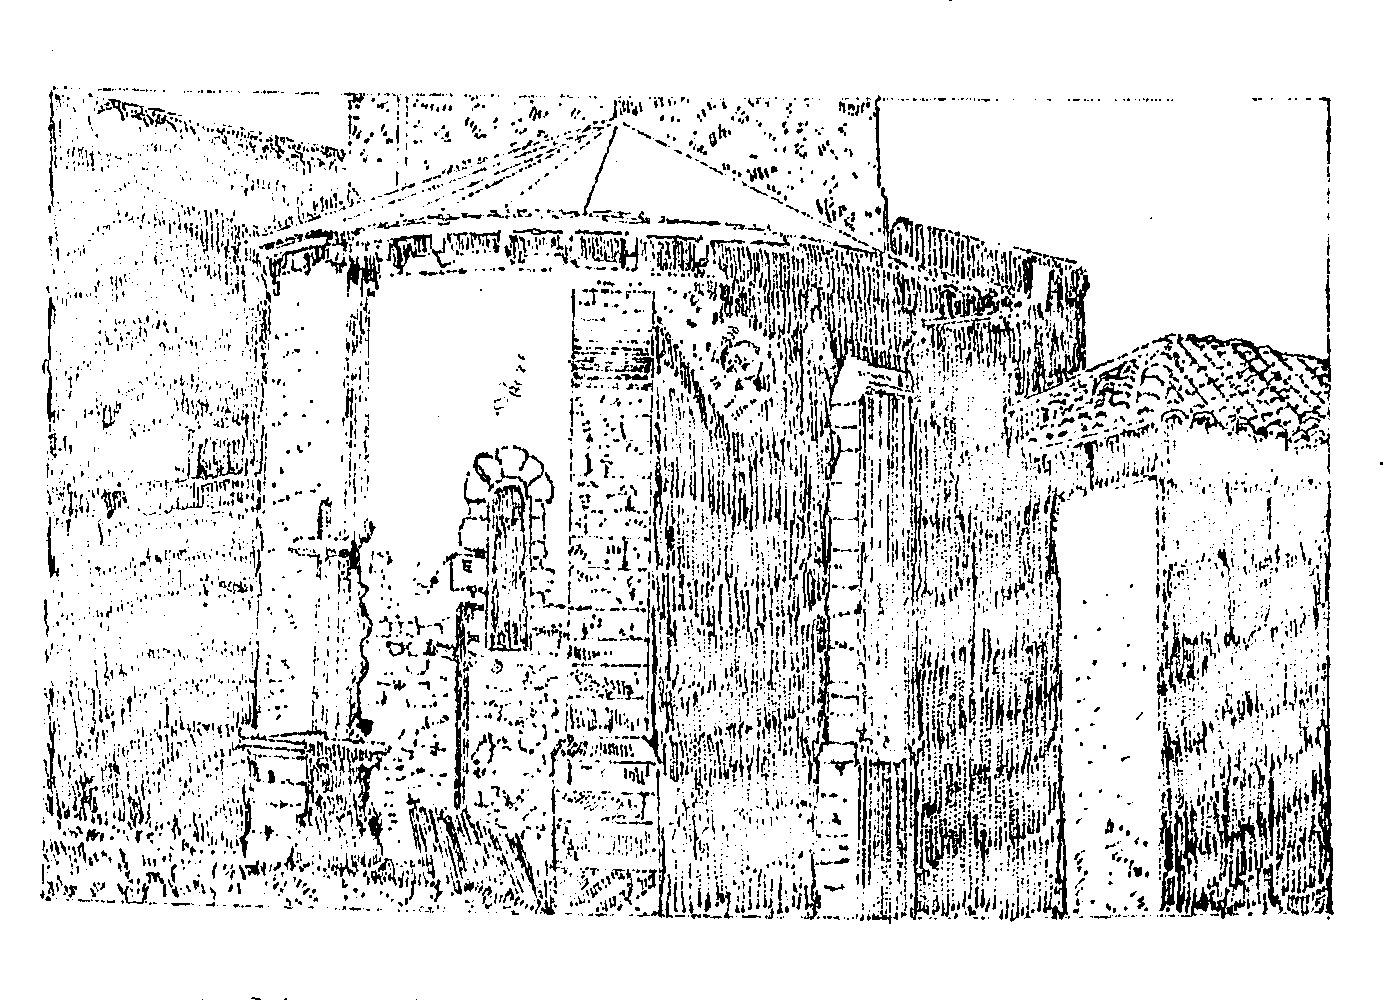
\includegraphics[width=0.62\textwidth]{Illustrations/illus-eglise-abside.jpg}\par
\ourouxcaption{Église d'Ouroux - Abside}\end{center}
% --- Page imprimée 184 — vue 187 (suite)
la même époque. Deux murs très simples, en pierres de la localité, sans contreforts, des fenêtres romanes sans aucun ornement ; le cintre de la grande porte retombant sur de simples pieds droits. La voûte elle-même était-elle ogivale ? Était-elle formée par une simple charpente ? On ne peut le dire. Dans les siècles derniers elle était lambrissée à compartiments selon l'usage du temps. Le lambris fut remplacé par un simple plafond avant la Révolution.

Quel contraste entre ce chœur que nous venons d'admirer et cette nef si pauvre au point de vue de l'architecture ! Il suffit pour en trouver l'explication de se reporter aux coutumes du Moyen Âge.

Lorsque des moines ou un bénéficier faisaient bâtir une église, ils ne construisaient que le chœur et le clocher. La nef était à la charge des paroissiens qui, la plupart du temps, très pauvres, ne faisaient que le strict nécessaire. Voilà le motif pour lequel nous n'avons dans nos paroisses de campagne aucune église complètement achevée : à un chœur fort régulier s'ajoute une nef d'une simplicité extrême.

Le bénéficier était tenu de pourvoir aux réparations du chœur et du clocher ; la conséquence est naturelle. Nous voyons cette loi appliquée à Ouroux jusqu'à la Grande Révolution. Le Chapitre de Beaujeu étant décimateur de la paroisse se voit contraint légalement par Mr Morin à faire les réparations urgentes au chœur de notre église et à son clocher et lorsque Mr Guillin lègue un bois à la fabrique il a bien soin de spécifier que les ais serviront aux réparations de la nef.

L'église d'Ouroux est parfaitement orientée, suivant l'usage de l'époque et les prescriptions liturgiques. La nef avait la longueur actuelle ; comme aujourd'hui l'aire du chœur était plus élevée que celle de l'église elle-même.

Étudions maintenant les transformations successives qu'elle eut à subir dans le cours des siècles.

Le chœur subit des transformations profondes. À une époque qu'il est impossible de préciser, peut-être sous l'administration de Mr Berthet, le maître-autel fut transporté du milieu du transept au fond même de l'abside. La forme semi-circulaire de celle-ci ne permet
% --- Page imprimée 185 — vue 188 (suite)
tant pas d'adosser l'autel contre la muraille, les colonnettes durent disparaître. On mura la fenêtre du milieu et l'autel ne se trouva plus éclairé que par les deux baies latérales.

Nous avons vu Mr Berthet, curé, faire une souscription afin de construire la sacristie du côté du maître-autel. Le sieur de Brossois fournit le ciment et le bois nécessaire pour le couvert. Du Ligier T'Estenoire donna la porte. Celle-ci était au même endroit qu'aujourd'hui. Il est probable que le transport de l'autel dut avoir lieu la même année, c'est-à-dire en 1683 ; toutefois la dépense faite par cette modification n'a point été relatée.

Peut-être même remplaça-t-il l'ancien autel par un nouveau. Du moins, nous le voyons acheter, au prix de 120 livres, cette même année un tabernacle fourni par Mr Novil, maître sculpteur demeurant devant le grand collège à Lyon. Il acheta en même temps les figures de St-Antoine et de St-Barthélemy qui furent placées dans leurs chapelles respectives.

Plus tard, comme il s'agissait de placer au-dessus de l'autel un grand tableau représentant les deux patrons de la paroisse et que la corniche, seul ornement d'architecture qui existait encore gênait, on la fit disparaître.

Mr Guillin devait à son tour poursuivre ces transformations si malheureusement commencées. Les deux fenêtres qui avaient été conservées de chaque côté de l'autel étant trop étroites pour donner une lumière suffisante furent, en 1763, l'une murée, celle de gauche, et celle de droite considérablement agrandie. On comprend facilement combien cet ensemble était disgracieux. Deux ans plus tard il faisait placer une statue à chaque angle de l'autel.

Les deux côtés du transept étaient occupés par les patrons de la paroisse : St-Antoine et St-Barthélemy. La chapelle du côté de l'épître était dédiée à St-Barthélemy ; celle du côté de l'évangile à St-Antoine.

Quel est celui qui dans les siècles passés eut la priorité ? Il ne subsiste sur ce point aucun document. Les titres les plus anciens ne mentionnent que le nom d'Ouroux (Oratorium). Ceux du XVème siècle emploient indifféremment St-Antoine et St-Barthélemy d'Ouroux ; St
% --- Page imprimée 186 — vue 189 (suite)
Barthélemy, St-Antoine d'Ouroux. En 1680 et pendant les années suivantes jusqu'à Mr Guillin les actes de catholicité portent toujours la mention St-Barthélemy d'Ouroux. En 1667 l'auteur du manuscrit beaujolais qui est conservé à la bibliothèque de Lyon s'exprime ainsi : « Ouroux ou Oratorium à cause de la dévotion qu'il avait à St-Antoine qui n'est qu'une chapelle dans l'église de St-Barthélemy où vient affluence de peuple de toute part… » Nous savons d'ailleurs que l'église de St-Vincent de Mâcon portait dans le principe le titre de St-Barthélemy. Rien de surprenant que notre paroisse qui dépendait directement du Chapitre de St-Vincent se soit mise sous la protection du patron primitif. La fête « belledoise » a toujours eu lieu comme aujourd'hui à la fête de St-Barthélemy. En 1632 Ouroux rayait à Melle de Montpensier à cause de sa seigneurie, à l'occasion de cette fête et des jeux de hasard auxquels on s'y livrait la somme relativement considérable de quinze livres.

Depuis le XVIIIème siècle St-Antoine ermite est devenu le principal patron de notre église. À la suite de quelles circonstances ce changement s'est-il opéré ? Sans doute à cause du pèlerinage dont il nous reste à dire quelques mots.

La chapelle de St-Antoine est depuis longtemps le but d'un pèlerinage célèbre dans nos contrées. Le 17 janvier, une foule considérable de pèlerins accourus de toutes les paroisses environnantes du Mâconnais comme du Beaujolais viennent implorer le Saint ermite à l'exemple de leurs pères. Comme du reste, dans tous les pèlerinages, c'était autrefois la coutume générale de venir à jeun. Pendant de longues années, un grand nombre, malgré les distances considérables qu'ils avaient à franchir, sont restés fidèles à ce pieux usage. Ils viennent aux pieds de notre saint patron accomplir les vœux faits par leurs ancêtres depuis plusieurs siècles, peut-être en faveur de leurs bestiaux et spécialement pour les porcs.

Quelle est l'origine de ce pèlerinage ? Il remonte certainement à une époque fort reculée. Dès 1667, comme nous venons de le voir, la chapelle de St-Antoine était le but « d'une grande affluence de peuple ». L'histoire nous permet de remonter plus haut encore. Le 1er octobre 1523, nous voyons le roi François Ier accorder par lettres patentes, au bourg d'Ouroux un marché tous les lundis de chaque semaine
% --- Page imprimée 187 — vue 190 (suite)
et deux foires par an, l'une huit jours après la St-Barthélemy, l'autre à la St-Antoine, le tout confirmé par le roi Charles IX. Cette foire établie, le jour de la fête de St-Antoine, nous permet de conclure qu'elle le fut à l'occasion du pèlerinage, les pèlerins voulant profiter de leur réunion à Ouroux pour leurs ventes et leurs achats.

On sait combien furent fréquents les pèlerinages, pendant la période du Moyen Age. Le peuple, avec son esprit de foi pratique invoquait d'abord Dieu et ses saints en face des fléaux si nombreux qui venaient l'éprouver à cette époque.

\begin{center}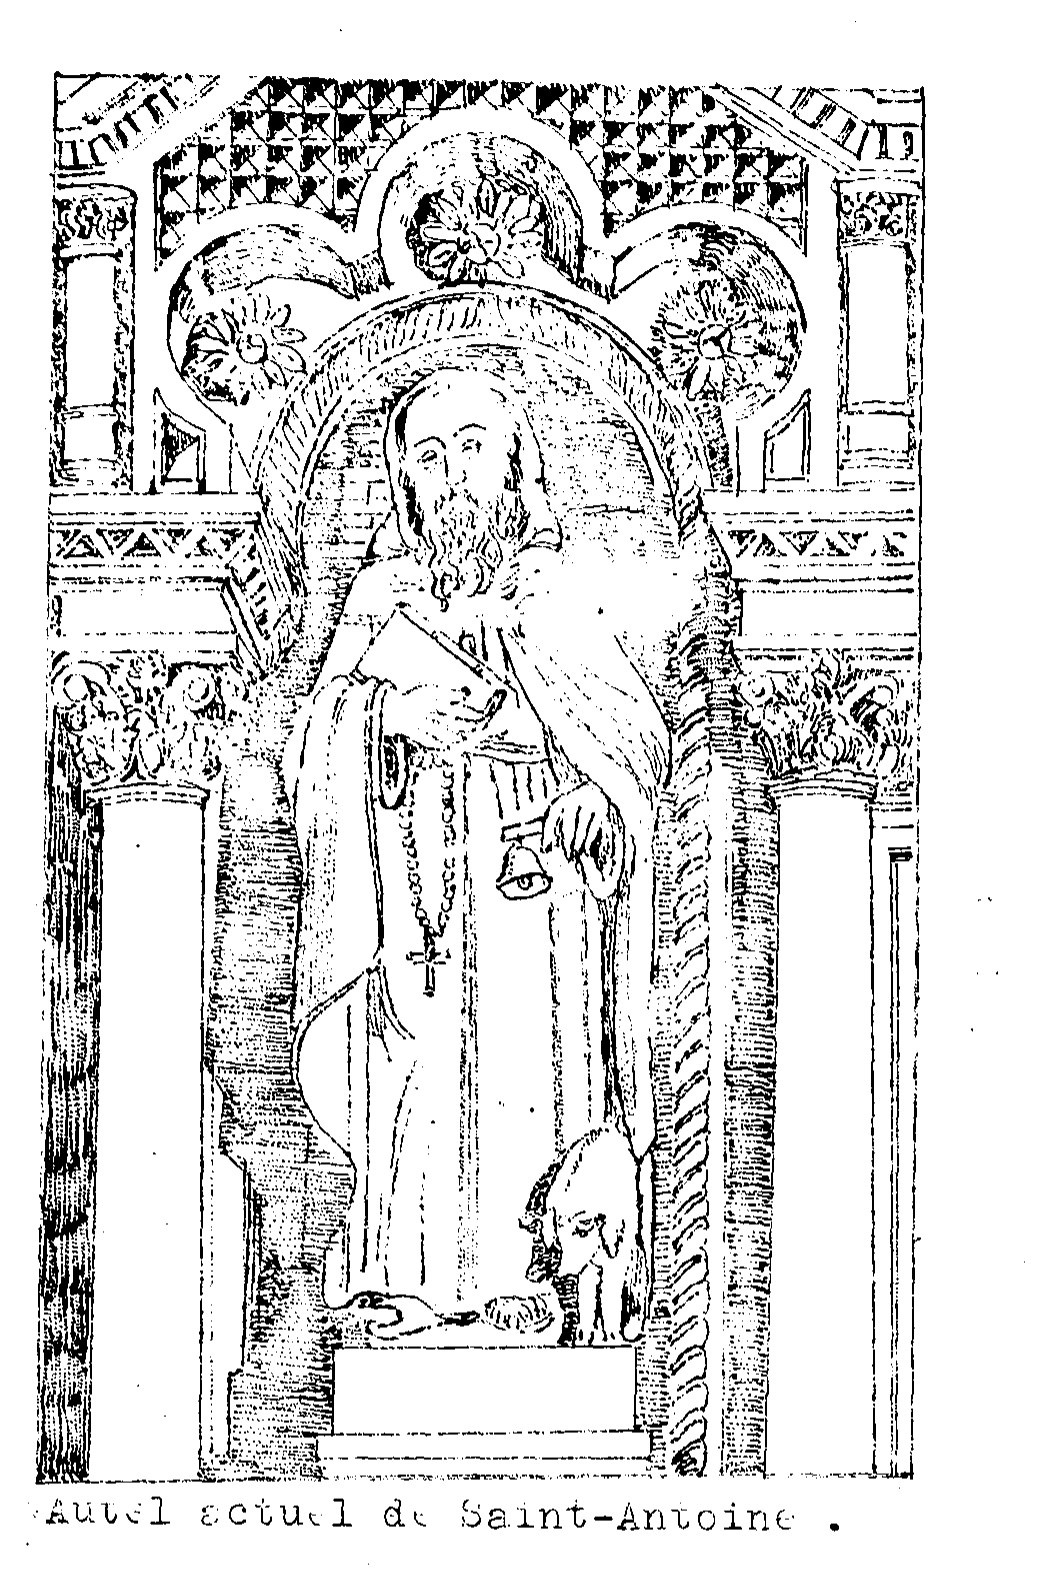
\includegraphics[width=0.62\textwidth]{Illustrations/illus-autel-saint-antoine.jpg}\end{center}

Une similitude, un simple rapprochement de nom, un attribut particulier, un emblème suffisait souvent pour fournir un point de départ à une dévotion particulière sur les motifs de laquelle l'Église n'avait point à se prononcer, dès lors qu'il n'y avait rien de répréhensible dans le but.

N'avons-nous pas encore actuellement le pèlerinage à la chapelle du château de Vers, paroisse de St-Igny, pour les enfants éprouvés par les vers ? À Julié dont la fête patronale est le jour de la Conversion de St-Paul. Le mot Conversion est devenu convulsion et par suite ceux qui se trouvent atteints d'une affection de ce genre ou qui craignent de le devenir se rendent en foule dans cette paroisse le 25 janvier.

Enfin n'avons-nous pas dans le Roannais un exemple d'une pareille anomalie ?

% --- Page imprimée 188 — vue 191
reille anomalie ? On appelle « tine » un tonneau qui sert à porter de l'eau et que les vignerons emploient pour porter la vendange. Or ils ont choisi comme protecteur de leurs vignes et par là même de leurs récoltes St-Jean-devant-la-porte-latine et par corruption Saint-Jean portant la tine et de fait on le trouve représenté avec une tine sur l'épaule.

La peinture nous représente St-Antoine portant un livre d'une main, de l'autre un bâton et une clochette ; à ses pieds un animal immonde ; auprès de lui du feu allumé.

Le livre rappelle que le saint solitaire avait une science merveilleuse des écritures ; le bâton que l'homme n'est ici-bas qu'un voyageur ; la clochette est le symbole de vigilance. Le feu indique l'efficacité de la protection du saint pour sauver des flammes de l'enfer ou du terrible fléau qui décima les peuples du Moyen-Age. Ce feu sacré, appelé aussi Mal des Ardents était une peste horrible appelée depuis « feu de St-Antoine ». Enfin personne ne l'ignore, l'animal immonde est la personnification du démon et des tentations violentes dont St-Antoine fut assailli par cet esprit impur.

Or qu'arriva-t-il ? Une épidémie, plusieurs peut-être causèrent de grands ravages parmi les troupeaux, ceux des porcs principalement. Les populations voyant cet animal représenté auprès de St-Antoine et par la peinture et par la sculpture, conclurent que ce saint en avait fait son compagnon fidèle. À cette heure encore, malgré les enseignements donnés sur ce point, le plus grand nombre n'affirme-t-il pas que St-Antoine avait toujours un porc auprès de lui dans le désert ? De là à l'invoquer spécialement pour obtenir de notre patron une protection efficace, il n'y avait qu'un pas.

Il s'était même établi dans ce pèlerinage un curieux usage. Chaque pèlerin apportait comme offrande un pied de porc qu'il déposait dans une corbeille placée à l'entrée de l'église. Le curé les distribuait ensuite aux pauvres de la paroisse. Cette coutume a subsisté jusqu'au commencement du XIXème siècle. Ce fut Mr Polloce qui la fit cesser vers 1920.

En 1869 la Chapelle de St-Antoine avait pour patron un laïc. Étant devenue vacante à cette époque, Sieur Gabriel de la Blanche, écuyer,
% --- Page imprimée 189 — vue 192 (suite)
seigneur du Post, La Tulle, Montaulieu et autres places obtint de l'évêque de Mâcon l'autorisation d'y fonder douze messes par an, au prix de six livres payables le lendemain de la St-Martin d'hiver ou bien encore dix sols après chaque messe acquittée. Le titre concernant cette fondation se trouve ci-après.

Une tradition prétend que cette chapelle servait de lieu de sépulture aux prêtres d'Ouroux. Elle semble difficilement conciliable avec l'acte de fondation de Charles de la Blanche. Comment se serait-il réservé la faculté de se faire enterrer lui et les siens dans sa chapelle, si déjà elle renfermait un caveau pour les curés ? Il semblerait donc que le lieu de leur sépulture dut être placé ailleurs, dans la chapelle de St-Barthélemy probablement puisque nous ne trouvons nulle part dans l'église un endroit affecté à cette destination et qu'il est certain d'après les actes de décès qu'ils furent inhumés dans un caveau spécial à l'église.

La nef, avons-nous vu, ne renfermait primitivement aucune chapelle. Mais à l'époque où les familles seigneuriales commencèrent à jouer un certain rôle dans la paroisse, quelques-uns tinrent à honneur de se distinguer du reste des fidèles en construisant des chapelles particulières. On pratiquait une ouverture dans les murs latéraux de la nef, on élevait une construction plus ou moins architecturale et on en fermait l'entrée par une grille afin que personne n'y pût pénétrer. Le seigneur faisait en même temps une fondation de messes à l'acquit desquelles avait droit le prêtre désigné par le fondateur ou ses héritiers.

Donnons sur ces diverses chapelles, telles qu'elles existaient à l'époque de leur disparition les détails les plus essentiels.

À droite, côté de l'épître, en allant du sanctuaire à la grande porte nous trouvons :

1° la chapelle de Sainte Croix  
2° la chapelle de Saint Claude  
3° la chapelle de Saint Vincent

À gauche du côté de l'Évangile, en suivant le même ordre :

1° Notre-Dame de Gré, St-Roch et St-Sébastien  
2° la chapelle de Sainte Magdeleine  
3° la chapelle de Ste-Catherine

% --- Page imprimée 190 — vue 193
\begin{center}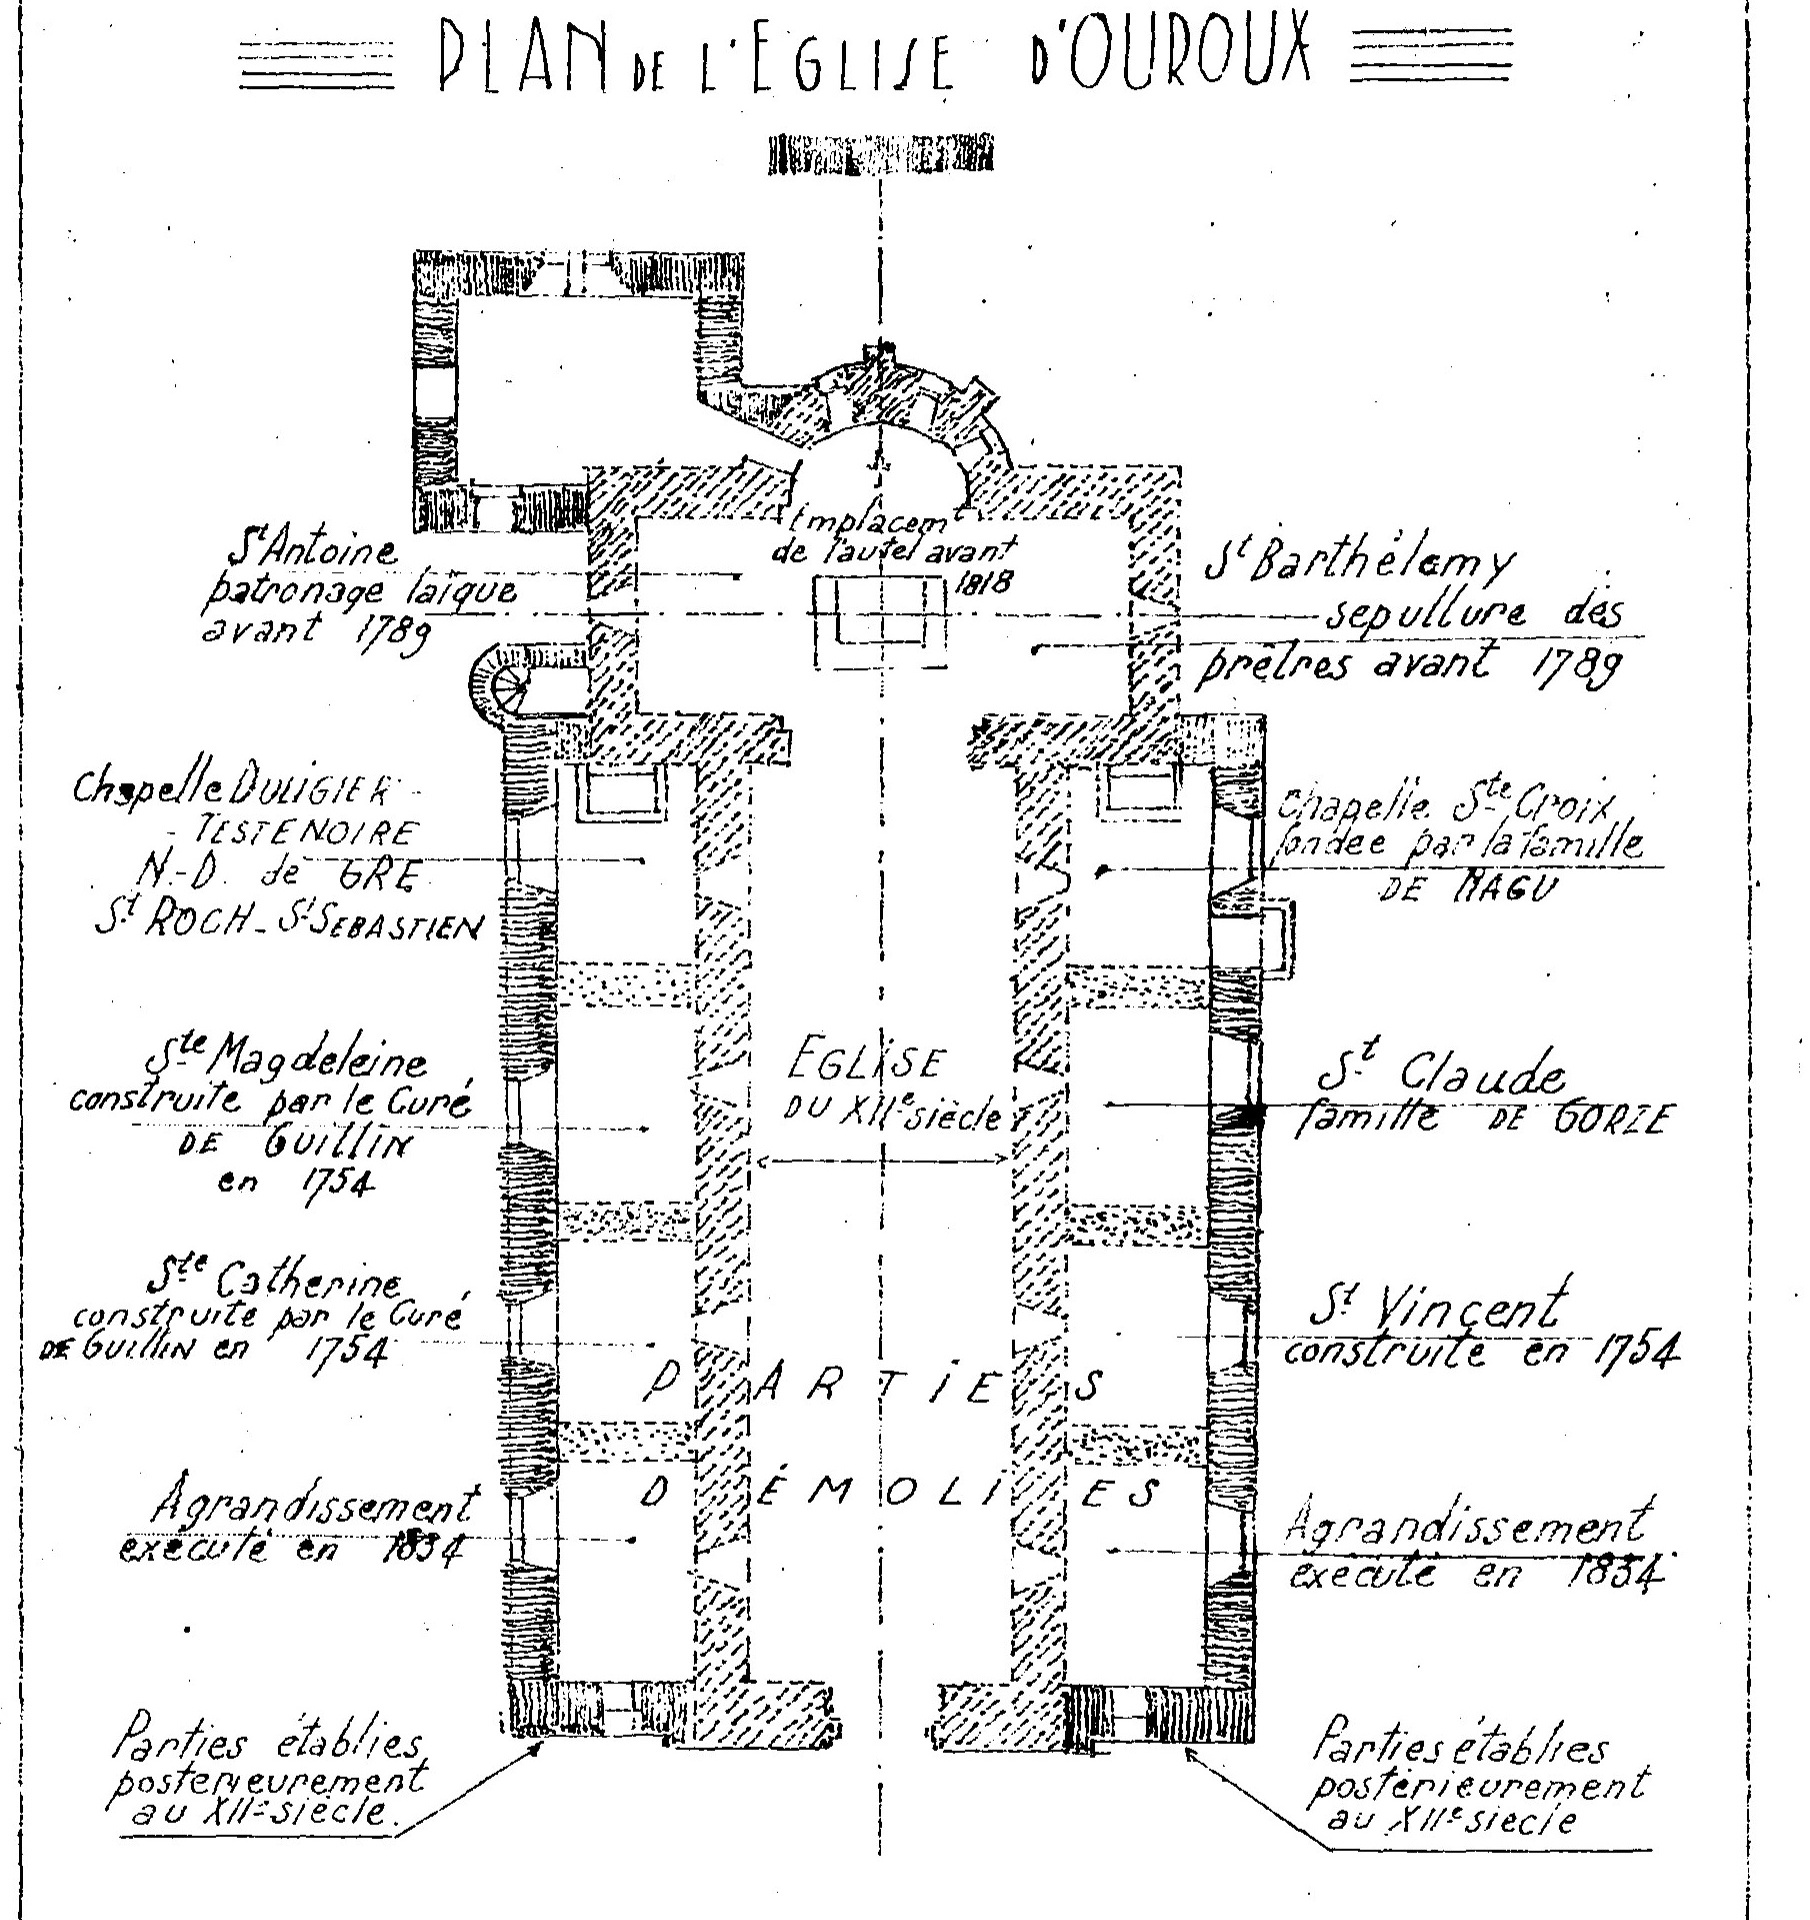
\includegraphics[width=0.62\textwidth]{Illustrations/illus-plan-eglise.jpg}\end{center}

D'après le plan dressé par LE MALL, Architecte —  
Le 30 Octobre 1903.

% --- Page imprimée 191 — vue 194
Aujourd'hui devenue chapelle de St-Antoine.

Nous possédons un extrait du titre de fondation faite par Thomas de Bosco, notaire à Ouroux, le lundi quatrième jour de juillet 1469. Cette expédition fut faite par Mr Perrichon, notaire royal à Lyon le 5 mai 1760. Le copiste ne connaissant probablement pas le latin et l'original lui-même offrant sans doute quelques difficultés à la lecture, le texte qui nous a été conservé est très défectueux dans certaines parties, le latin rempli de fautes qui en rendent le sens presque incompréhensible. Voici néanmoins une analyse aussi fidèle que possible de cet acte, le plus ancien qui nous soit parvenu sur notre église.

« Honnête et prud'homme, Thomas de Bosco, clerc notaire public de  
« la paroisse des saints Antoine et Barthélemy d'Ouroux, bourg du  
« Beaujolais, diocèse de Mâcon, par la grâce de Dieu, sain d'esprit  
« quoique débile de corps à cause de la vieillesse, sachant que  
« rien n'est plus certain que la mort et que rien de plus incertain  
« que son heure… craignant de quitter ce monde sans avoir  
« porté remède au salut de son âme et de celle de ses bienfaiteurs,  
« parents et amis, et surtout de l'âme de son père, de sa  
« mère et de son épouse et de celle de vénérable messire Jehan de  
« Carelia prêtre et son parent dont il a été l'héritier universel…  
« à la gloire et à l'honneur de Dieu le Père tout-puissant  
« et de la très glorieuse Vierge Marie et de toute la cour céleste.  
« …cède et donne… aux vénérables messieurs les curés des  
« églises paroissiales de St-Barthélemy et St-Antoine d'Ouroux, de  
« Sainte-Marie d'Avenas et de St-Mamert et à leurs successeurs  
« qui acceptent… savoir :  
« Au curé de St-Mamert trois blancs royaux valent quinze deniers  
« tournois pour célébrer chaque lundi une messe de mort dans la  
« chapelle fondée dans l'église de St-Barthélemy d'Ouroux et ap-  
« partenant audit Thomas de Bosco.  
« Au curé de St-Antoine et St-Barthélemy d'Ouroux pour célébrer  
« tous les mercredis, au lever du soleil, une messe en l'honneur  
« du St-Esprit, quatre blancs royaux valent quinze deniers tour-  
« nois.  
« Au curé d'Avenas, trois blancs royaux valent quinze deniers tour-  
« nois pour chaque messe qu'il devra célébrer par lui-même ou  
« par son vicaire chaque samedi, dans ladite chapelle en l'honneur  
« de la glorieuse Vierge Marie.  
« Le curé d'Ouroux sera tenu de fournir pour chacune de ces mes-  
« ses les hosties, le vin, les cierges et les ornements ; il reçoit  
« à cet effet pour sa messe un blanc royal de plus que les deux  
« autres… et lorsque ses héritiers à Ouroux paieront, après  
« chaque messe le prix stipulé ci-dessus, le célébrant sera tenu  
« de réciter sur le tombeau du fondateur qui existe sous la cha
% --- Page imprimée 192 — vue 195 (suite)
« pelle, le psaume De Profundis avec les oraisons et versets accoutumés pour le salut de son âme et de celles de ses parents et amis… le donateur consacre à cette fondation les rentes, cens et servis à lui dus par ses fermiers et consignés dans ses terriers »

Vient ensuite l'énumération des rentes qui lui sont dues sur la paroisse de Montchout (Monsols), les Ardillats, St-Christophe, Trades, St-Mamert et Ouroux. De plus, il hypothèque tous « ses biens, maisons et édifices qu'il peut avoir » in villa Oratorii (dans le bourg d'Ouroux) aux Friauts (les Friats), au Clapier et à la Fosse.

L'acte fut passé au lieu de la Condemne le lundi 14ème jour du mois de juillet de l'an 1449 en présence de discrètes personnes Jean Champagnon curé de St-Christophe, Jean l'un curé de Montchout, Jean de Fillialibus prêtre et André Boniface clerc notaire, par devant Benoit de Certa prêtre curé de Trades.

Suit l'approbation de l'autorité diocésaine. Pierre Aliseti licencié en l'un et l'autre droit, officiel de Mâcon, après avoir visité la chapelle construite de nouveau dans l'église d'Ouroux en l'honneur de la Sainte Croix par Thomas de Bosco, notaire public, a constaté qu'il s'y trouvait un autel de marbre avec une pierre sacrée également en marbre ; que la chapelle était pourvue des ornements nécessaires, d'un missel et d'un calice. Énumérant ensuite les diverses conditions et charges de la fondation, il l'approuve absolument.

Cette visite eut lieu le Dimanche avant la fête de la Toussaint, l'an 1449 (ici le copiste écrit : anno millesimo quadraginta nono, quadragesimo sexto, l'an 1449,406) en présence de Mr Jean Lemontalino vicaire dudit lieu, de Thomas Pélissard maréchal, Jean Massoheril ou autrement de Laye et plusieurs autres paroissiens d'Ouroux.

Ce dernier acte nous permet de conclure que la chapelle était très ancienne, puisque Thomas de Bosco n'en est point le fondateur proprement dit, mais bien le restaurateur. L'expression « de novo constructam et aedificatam » ne permet pas d'en douter. Mais par qui fut-elle fondée ? Sans doute par la famille de Nagu, famille remontant au XIe siècle et dont le berceau fut précisément le bourg d'Ouroux.

Nous savons d'ailleurs, par l'histoire des croisades qu'un de ses membres, Henri de Nagu se croisa et qu'il se trouvait à Acre en 1240. Il est probable qu'à son retour dans sa patrie, pour conserver le souvenir
% --- Page imprimée 193 — vue 196 (suite)
de son voyage en terre sainte, peut-être aussi pour honorer quelque relique de la vraie croix rapportée de Jérusalem, fit-il construire cette chapelle à laquelle il donna le nom de Sainte Croix. Lorsque le fief de Nagu fut démembré et acheté par différents seigneurs, de Bosco, acquéreur de la partie du fief située au bourg même entra ainsi en possession de leur chapelle qu'il fit réparer ensuite.

Les dernières volontés de Thomas de Bosco furent-elles longtemps exécutées ? Il est probable que le passage des protestants à Ouroux apporta quelques troubles dans l'accomplissement de ces diverses fondations. En 1670 Mr Morin, curé de la paroisse, entreprit de régulariser les choses. Demoiselle Jacqueline de la Ronzière, veuve de Philibert des Brosses sieur du Bessay et des Collettes, possédant une partie des biens situés à St-Christophe près de Tréssavin et de Bacot, qui avaient appartenu autrefois à Thomas de Bosco voulut faire valoir ses droits au patronage de cette chapelle. Mr Morin refusa ; de là le procès en la sénéchaussée et siège présidial de Lyon. Mr Morin prétextait la nullité de l'acte qui était entre les mains de Jacqueline de la Ronzière. Quelles preuves fournissait-il ? Je l'ignore. La sentence dut lui être favorable, car, à partir de cette époque, nous ne trouvons aucune mention de fondation dans cette chapelle.

La chapelle de Sainte Croix portait à la fin du XVIIIème siècle le titre de Notre Dame des Sept Douleurs.

La voûte en ogive très aiguë rappelle parfaitement l'époque à laquelle elle fut construite par Thomas de Bosco. Mr Guillin fit agrandir la fenêtre de cette chapelle en même temps que celles des chapelles de St Antoine et de St Barthélemy.

Ce fait confirme la conclusion émise plus haut : la chapelle de Sainte Croix avait eu pour fondateur primitif l'ancienne famille de Nagu. La fenêtre que Mr Guillin fit agrandir n'était évidemment pas de la même époque que la voûte puisqu'elle n'appartenait ni au style rayonnant, ni au style flamboyant comme cela aurait dû avoir lieu si elle avait été construite par de Bosco. C'était une fenêtre étroite, comme celle du transept et de l'abside.

% --- Page imprimée 194 — vue 197
Cette chapelle fut construite immédiatement à la suite de celle de Sainte Croix par la famille de Gorze, famille célèbre dans nos contrées et qui tirait son nom du fief de Gorze situé sur la paroisse de Germolles.

La voûte était ogivale avec arceaux, pendentif et supports des arceaux historiés. La fenêtre qui subsiste encore nous rappelle la plus belle période du style ogival flamboyant. Le réseau qui en remplit le tympan est formé de lignes ondulées, prismatiques ; un meneau décoré de moulures très simples la partage en deux parties. Elle était ornée de deux vitraux à personnages qui furent brisés à une époque inconnue. Cette fenêtre est l'unique objet qui ait été respecté dans les multiples réparations qui ont fait disparaître de notre église les souvenirs des siècles passés.

À quelle époque remonte la fondation de la chapelle Saint-Claude ? L'acte rapporté ci-après est le seul titre qui puisse nous fixer à ce sujet. Cette chapelle fut fondée par Messire Michel Bertet, un des membres de la famille de Gorze et dont les ancêtres (ou lui-même) durent acquérir, en même temps que Thomas de Bosco, une partie du fief démembré de Nagu. Les seigneurs de Gorze possédèrent à la suite de cette acquisition la partie du bourg, située sur la rivière de Grosne, tandis que de Bosco possédait la partie située sur le chemin du pont (les Chassagnes à « la croix du rempart »). De Bosco ayant une chapelle, la famille Bertet ne pouvait moins faire que d'en construire une à son tour.

En 1689, le patron de cette chapelle était Philibert Bertet chevalier seigneur de Gorze, la Salle, Germolles et autres lieux ; il en était aussi le nominateur. Cette même année le titulaire du bénéfice était Claude de Thivault, et l'abbé Despré, doyen du chapitre d'Aigueperse, qui démissionna le 17 octobre 1789. Le 14 novembre suivant Messire Elzéard Bertet, curé d'Ouroux installa comme titulaire noble Philibert Antoine Bertet confrère de l'Oratoire de Jésus.

Aucun titre ne nous indique les conditions de cette fondation. En 1765 les messieurs de Gorze étaient encore patrons de cette chapelle ; un abbé de Serrière en était chapelain. Il obtint une réduction
% --- Page imprimée 195 — vue 198 (suite)
de service qui fut une messe le samedi de chaque semaine et six messes les six derniers mercredis de l'année. Ces cinquante-huit messes furent transportées à Mâcon avant la Grande Révolution. Le caveau qui existait sous la chapelle a été conservé.

\ourouxsubtitle{CHAPELLE DE SAINT VINCENT}

Mr Guillin, dans le but d'agrandir l'église qui était insuffisante pour la population fit construire à la suite de la chapelle de Gorze une autre chapelle à laquelle il donna le titre de Saint-Vincent, patron du diocèse de Mâcon. La voûte était à plein cintre et sans ornement : elle n'offrait rien de remarquable.

Du côté de l'Évangile, nous avons en premier lieu la chapelle de :

\ourouxsubtitle{NOTRE DAME DE GRE (ou GREZ) St-ROCH et St-SEBASTIEN}

Elle appartenait à la famille Duligier-Testenoire. Mr Guillin, ayant mis en doute la réalité de leurs droits, exigea de Jean-Marie Duligier des titres en forme que celui-ci ne pouvait fournir. Voici comment s'exprime Mr Guillin dans un placard concernant les fondations et affiché à la sacristie en 1765 : « La chapelle de Notre-Dame de Gre située dans l'église d'Ouroux a été un titre de bénéfice de patronage laïc. Les Testenoire rappellent en 1707 ces anciens titres pour avoir les honneurs de la chapelle mais ils ne les montrent pas ».

Voici, en effet, quelle était la réponse donnée par J. M. Duligier.

« A la requête du sieur J. M. Duligier contre Guillin curé d'Ouroux, démontré : que de temps immémorial ledit sieur Duligier par lui et ses auteurs possède dans l'église paroissiale d'Ouroux une chapelle, placée du côté de bize et dont il a le droit de patronage de la dite chapelle, étant sous le vocable de N. D. de Grez, St-Roch et St-Sébastien ; l'existence de cette chapelle est prouvée par un titre en forme de narration de l'année 1575, les vestiges de la fondation primitive étant perdus dans l'obscurité des temps ». Dans la fondation des cinq messes ci-dessous mentionnées, les fondateurs disent : « sous réserve expresse de leurs droits de nomination, collation et d'ensepulture ».

La question qui avait été soulevée dès l'année 1742 n'avait encore reçu aucune solution comme on le voit en 1765.

% --- Page imprimée 196 — vue 199
Le 22 septembre 1743, Benoit Duligier étant mort, Mr Guillin consentit de l'inhumer dans la chapelle de N. D. de Grez, sur la promesse de la part de J. M. Testenoire de ne point s'appuyer sur le fait de cette sépulture pour prouver ses droits sur la chapelle, mais de se mettre en mesure d'en apporter des preuves concluantes dans le délai de trois mois. Le père ayant refusé d'admettre ces conditions l'enfant fut enterré au cimetière. Le 9 décembre de l'année suivante, sa fille meurt âgée de 12 jours. Elle est enterrée dans la chapelle, sans préjudice de jugement que Mgr l'évêque de Mâcon portera sur la question en litige.

La sentence de l'évêque fut, sans doute, favorable à Duligier puisque celui-ci fit faire diverses réparations à sa chapelle en 1766. Elle empiétait de trois pieds de largeur sur onze de longueur sur la nef. Afin de laisser plus d'espace à celle-ci, il transporta l'autel au fond même de la chapelle. Deux caveaux étaient destinés à recevoir les membres de la famille. Le balustre qu'il y avait fait placer pouvait facilement s'enlever pour les inhumations. Ayant fait mettre à cette époque une serrure au balustre, Mr Guillin l'enleva le dimanche suivant. Cette serrure fut replacée le 7 octobre 1766, en vertu d'une ordonnance de l'évêque de Mâcon.

Le 28 mars 1667, Messire Pierre Reyras, curé de Cenves, chapelain et prébendier de la chapelle de Notre Dame de Testenoire, prébende obtenue de Messire Pierre Testenoire le 7 juin 1656, fut installé par Mr Chrysostome Morin, vicaire perpétuel d'Ouroux. La chapelle était vacante par suite du décès de Guillaume Testenoire, curé de St-Lager, issu des Testenoire de Beaujeu et qui était prébendier. L'acte de prise de possession conservé aux archives de Mâcon, série B, N° 441, a été reçu par Mr de la Sarre, notaire royal à Cenves. Les témoins sont : Delhome ; Morin prêtre, Lubost et Testenoire.

Passons maintenant au titre signalé plus haut et concernant la fondation faite par Jean Duligier et Jean Chrysostome Duligier.

Par acte reçu à [ILLISIBLE: Abillon] notaire royal, ils fondèrent à perpétuité cinq messes basses qui devaient être dites à l'autel de la chapelle. Lesdits fondateurs étant du côté de l'Évangile et, au-dessous, de
% --- Page imprimée 197 — vue 200 (suite)
celle de St Antoine sous le vocable de N.D. de Gré, St Roch et St Sébastien, avec un « De Profundis » et un « Libera me » à voix basse, aspersion à l'eau bénite après chaque messe, le premier mardi du mois de décembre, mars, mai, juin, juillet et septembre. La première en l'honneur du St-Esprit, la seconde en l'honneur de St Jean et St Hugues, la troisième en l'honneur de la Sainte Vierge Marie, la quatrième de St Roch et St Sébastien, la cinquième de St Jean Chrysostôme. » Pour cette fondation ils donneraient à messire curé et à ses successeurs un champ situé près du cimetière qui fut vendu en 1793 et racheté par la fabrique d'Ouroux.

Cette chapelle n'offrait rien de remarquable. La voûte était à plein cintre et plus basse que celles des autres chapelles. On y voyait un tableau représentant St Roch et St Sébastien aux pieds de la Sainte Vierge portée sur un nuage et tenant l'enfant Jésus. On a écrit que ces deux personnages étaient des portraits de deux membres de la famille des Testenoire. C'est là une erreur puisque l'un des deux St Roch était représenté avec le bourdon du pèlerin. Au bas du tableau étaient les armes des Dulligier :

D'azur, à trois flèches d'or en pal accompagnées en pointe d'un cœur de même ; au chef d'argent chargé d'une tête de sable, accostée de deux étoiles d'azur.

Le prieuré des Testenoire d'Ouroux n'ayant pas d'armoiries, aucun titre du moins n'en fait mention, celles qui étaient sur le tableau devraient être les armes des Testenoire de Jacot. Le tableau devait être par conséquent un don de cette famille à la chapelle des ancêtres. Tombé de vétusté il a disparu vers 1930 ainsi que la chapelle.

\ourouxsubtitle{CHAPELLE de Ste MAGDELEINE -- CHAPELLE de Ste CATHERINE}

Ces deux chapelles furent construites à la suite de la précédente par Mr Guillin vers 1754 en même temps que celle de St-Vincent.

\ourouxsubtitle{CHAPELLE DE SAINT JEAN BAPTISTE}

Cette chapelle dont nous possédons le titre de fondation ne fut point construite. Pour quel motif ? nous l'ignorons. Elle eut pour fondateur Jean Montel marchand, habitant du bourg d'Ouroux et Antoinette
% --- Page imprimée 198 — vue 201 (suite)
Richard, sa femme. Elle devait être construite à la suite de la chapelle Dulligier, le long de la muraille. Il leur était concédé 8 pieds de long et 6 pieds de large avec permission de l'entourer d'une balustrade, de la fermer à clef et d'y avoir leur sépulture. Ils avaient également la faculté de percer la muraille et de construire leur chapelle en dehors de la nef ; dans ce cas ils perdaient tout droit à la concession faite à l'intérieur de l'église.

L'acte de fondation est du 17 mai 1668. Michel Colbert évêque de Mâcon l'approuve ; le 28 du même mois, à Chenas, pendant sa visite pastorale. Jean Montel et sa femme fondèrent dans leur chapelle douze messes par an qui devaient être dites aux conditions suivantes :

« 4 messes pendant l'octave de St Jean Baptiste, la cinquième le second juillet, jour de la visitation que St Jean fut sanctifié dans le sein de sa mère Sainte Elisabeth ; la sixième le vingt neuvième aoust jour consacré au martyre de saint Jean baptiste ; la septième le lendemain de la feste des roys vingt-cinq janvier, temps auquel Notre Seigneur baptiza Saint Jean et mérita le nom de Baptiste ; la huitième le jour de Saint Marcel seizième janvier veille de Saint Antoine hermite ; la neuvième le jour de Saint Antoine de Padoue ; la dixième le jour de Saint Crespin ; la onzième et la douzième messes seront dites à pareil jour du décès desdits fondateurs, avec les De Profundis et l'oraison Fidelium ; avec aspersion d'eau bénite »

Ils s'engagèrent eux et leurs successeurs à payer 10 sols par messe ou 6 livres par an qu'ils hypothéquèrent sur leur pré « La Turche ».

Par son testament du 8 mars 1674, Antoinette Richard femme de Jean Montel fonda dans la même chapelle, une messe des trépassés qui devait être dite tous les lundis au prix de 7 sols.

J'ai dit que cette chapelle n'a jamais été construite, extérieurement du moins, car elle semble avoir existé dans la nef, selon l'acte de fondation, du moins pendant quelques années. Nous pouvons le conclure d'une observation consignée dans un « état des revenus de tous les gentilshommes exempts, privilégiés et habitants qui possèdent des biens dans la paroisse d'Ouroux » et où nous lisons :

« Les héritiers du dict Montel possèdent dans l'église d'Ouroux une chapelle qui occupe 12 pieds de long sur 7 pieds de large de ladite nef. Ils sont obligés de la réparer ainsi que le lambris et le carreilage. Prière à l'intendant de les taxer pour les dites réparations. »

Toutefois cette chapelle n'a laissé dans notre église aucune trace.

% --- Page imprimée 199 — vue 202
\ourouxsubtitle{CONCESSIONS dans L'ÉGLISE}

On concédait aux familles, moyennant une redevance annuelle, l'emplacement d'un tombeau dans la nef de l'église. La concession comprenait un espace de 7 pieds de long sur 4 de large, avec la faculté d'y placer une pierre de la largeur de 3 pieds et 4 de longueur. Elle était faite à perpétuité et tous les membres de la famille avaient le droit de s'y faire inhumer. Voici à quelles conditions ; le concessionnaire devait entretenir en bon état le pavé de carreaux en pierres de taille, le lambris et le couvert correspondant à l'espace concédé ; le mur devait être blanchi de fond en comble. En 1679 la somme à payer annuellement était de 10 sols ou une demi-livre de cire jaune au choix du fabricateur.

On comprend facilement l'intérêt qu'avait la paroisse à aliéner ainsi certaines parties de l'église. L'entretien de la nef étant à sa charge et ses ressources lui permettant difficilement de subvenir aux dépenses que nécessitaient les réparations, la fabrique diminuait donc considérablement ses charges en les répartissant entre les divers concessionnaires.

Les actes qui nous sont parvenus ne nous mentionnent qu'un petit nombre de familles ayant obtenu une concession : Claude de la Place et Morin son gendre ; Claude Cinquin et Benoît Jambon, son gendre ; Geoffroy Trousset, tailleur d'habits, vers la fin du XVIIIe siècle.

Nous trouvons néanmoins plusieurs sépultures dans l'église entre autres celles des membres de la famille de Gros-Bois, celle de Françoise de Macé, veuve de messire de Montrichard, seigneur de la Brosse à St-Igny, décédée à Ouroux le 2 mai 1707.

Il est donc à présumer que le nombre des concessions était beaucoup plus considérable.

% --- Page imprimée 200 — vue 203
L'église était précédée d'une espèce de porche qui portait le nom de Gallonière. Le toit était soutenu par deux colonnes. Sur l'une d'elles on lisait l'inscription suivante en vieux français :

« En tot ce que tu feires, regarde la fin. »

L'inscription de l'autre colonne ne nous a pas été conservée. Ces colonnes en pierres ont été enfouies dans les fondations lors de l'agrandissement de l'église. La partie de la façade placée sous la Gallonière était couverte de fresques représentant les protestants abreuvant leurs chevaux dans le bénitier. Mr Trouilloux les fit recouvrir d'un badigeon, sous prétexte d'inconvénience.

Le clocher qui surmonte la coupole se termine en pyramide quadrangulaire. Jusqu'en 1836 il fut couvert en tuiles creuses. Bien que d'une construction massive, il offre néanmoins un aspect monumental avec ses deux étages de fenêtres géminées dont les arcs viennent reposer sur deux colonnettes surmontées de chapiteaux ornés eux-mêmes de feuilles grossièrement sculptées. Trois colonnes cylindriques à demi engagées dans le mur ornent chaque face de l'étage supérieur. Comme nous l'avons vu, le clocher renfermait quatre cloches avant la grande révolution, trois d'entre elles disparurent à cette époque.

En 1839 les deux cloches achetées par Mr Trouilloux furent cassées ; l'auteur de ce dégât croyait avoir à se venger de la conduite de Mr Polloce à son égard. On se mit en mesure de les remplacer. À cet effet un accord fut conclu avec Mr Jean Claude Jurdin, fondeur à Lyon, qui s'engagea à prendre le métal des deux anciennes cloches au prix de 1 f 20 la livre et pesant environ 1000 kilos et à en fournir deux autres au prix de 1 f 60 le ½ kilo.

Le 24 septembre 1839 elles furent baptisées par Mr le curé de Monsols délégué par Mgr l'Archevêque de Lyon.

La première reçut le nom de Antoinette Françoise. Le parrain fut Mr le baron Jean Marie de la Roche Lecarelle et la marraine Mme la baronne de la Roche Lecarelle, représentés par Mr Antoine Dulligier, maire et Marie Françoise Michon, femme de Mr Duranton, notaire et adjoint d'Ouroux. Elle porte comme inscription :

% --- Page imprimée 201 — vue 204
« Venite filii audite me ; timorem Domini docebo vos »

« Venez mes enfants, écoutez moi : je vous enseignerai la crainte du Seigneur ».

Puis viennent les noms du parrain et marraine. Elle pèse 735 kgs.

La seconde a reçu le nom de Anne Marie Angèle : elle pèse 564 kgs.

Le parrain fut : Mr Jean Marie Victor Dauphin de Verna ; la marraine : Anne Pierrette Angèle de Lubac, Vve Guillin d'Avenas. L'inscription :

« Vespere et mane et meridie orabo et annuntiabo laudem Domini et exaudiet vocem meam »

« Le soir, le matin et à midi je prierai et je chanterai les louanges du Seigneur et il écoutera ma voix »

La troisième a été bénite le 1er mars 1840 ; elle pèse 252 kilos.

Le parrain fut : Antoine Marie Dulligier Testenoire, maire et la marraine : Mme Adélaïde Joséphine Mahien, femme Guillin. Elle porte pour inscription ces mots du psalmiste :

« Laudate, pueri, Dominum »

« Enfants, louez le Seigneur »

Telle fut l'église d'Ouroux dans les siècles passés. Voyons ce qu'elle est devenue successivement jusqu'à nos jours.

Mr Trouilloux ne changea rien à la disposition intérieure lors du rétablissement du culte. Les ressources disponibles de la paroisse furent employées à l'achat des objets nécessaires au culte. Néanmoins l'église étant insuffisante pour contenir toute la population il fit construire sur la grande porte une tribune qui devait disparaître en 1830.

Aussitôt qu'il fut installé curé d'Ouroux, Mr Polloce se mit en mesure de rendre au chœur son ancienne régularité. Pour cela il transporta le maître-autel du fond de l'abside au centre même du transept au-dessous de la coupole. Jusqu'à ce moment le maître-autel comme les huit autels des chapelles était en bois orné de peintures grossières. Il en fit construire un nouveau en marbre de Tournus qui a coûté 660 frs. Les cordes des cloches qui traversaient la coupole durent par conséquent être transportées dans le bras du transept où elles sont encore.

% --- Page imprimée 202 — vue 205
\begin{center}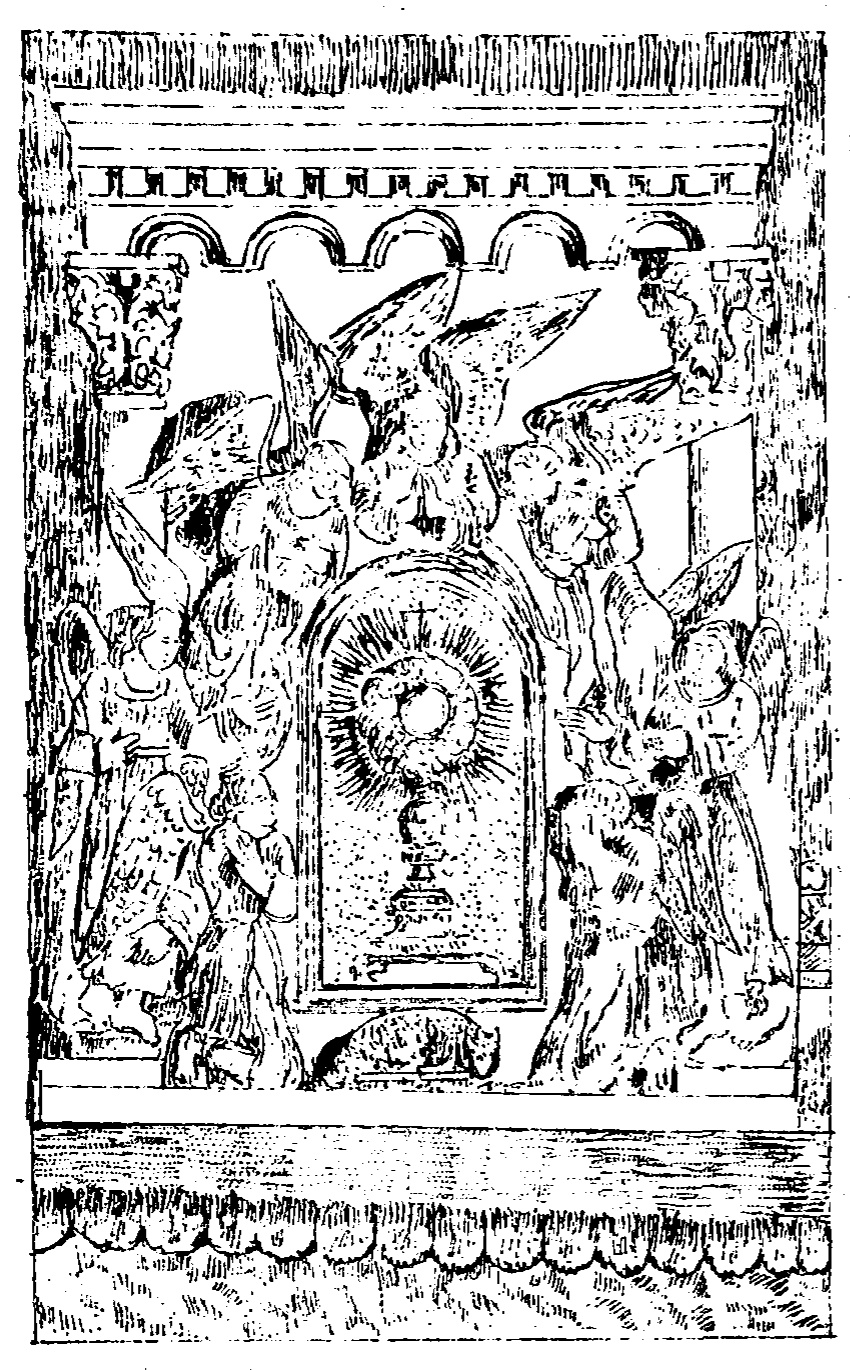
\includegraphics[width=0.62\textwidth]{Illustrations/illus-tabernacle.jpg}\end{center}

Le tabernacle a été sculpté par Mr l'abbé Morétain, du moins dans ses parties principales.

Son départ pour la terre sainte ne lui ayant pas permis de terminer ce travail, un sculpteur lyonnais, Mr Sabit, fit l'agneau qui est au pied du tabernacle, les chapiteaux, l'entablement et le personnage qui est debout derrière l'autel. Donnons une description sommaire de cette œuvre.

Sept anges dans l'attitude de l'adoration, du respect et de l'amour entourent la porte en cuivre sur laquelle est figuré un ostensoir. Deux d'entre eux, à genoux sur le socle expriment l'étonnement et la crainte que le chrétien doit éprouver à la vue du mystère de la présence réelle. Deux autres, les ailes largement déployées et faisant saillie en dehors du tabernacle debout sur la base des colonnes et derrière les deux premiers, montrent Notre Seigneur Jésus-Christ. Le cinquième et le sixième sont en adoration. Le septième occupant le haut de la porte paraît sortir du tabernacle même ; il est dans l'attitude de la prière.

De chaque côté, deux anges à genoux remplissent presque complètement les faces latérales, exprimant, eux aussi, leur étonnement et invitant les hommes à approcher.

Quatre colonnes supportent l'entablement qui repose à faux sur les chapiteaux hors de proportion eux-mêmes avec le monument. Les règles de l'anatomie ont été fort peu respectées dans la pose des personnages ; les dispositions des deux anges du milieu surtout sont très défectueuses.

Mr Pollosse, suivant en cela l'inspiration de Mr Morétain, demanda au sculpteur lyonnais de représenter sur la partie postérieure de St-Jean-Baptiste montrant Notre Seigneur. Cette condition n'a pas été remplie ; on y voit un personnage allégorique représentant la Charité qui tient entre ses mains une sorte de ciboire d'où s'échappent des flammes. Il est drapé à l'antique. L'expression des traits de la figure contraste avec la piété, le calme des anges sculptés par Mr Morétain et il n'est pas nécessaire d'un examen bien attentif pour constater qu'il y a eu, dans l'exécution de cette œuvre, le concours de deux mains diversement inspirées.

% --- Page imprimée 203 — vue 206
Dans ce tableau tout est vivant. Sur le visage de chacun de ces anges se reflètent, pour ainsi dire, les sentiments intérieurs dont ils sont animés. Cette partie de l'œuvre rachète et fait oublier les inexactitudes de détail qui se rencontrent dans l'exécution.

Les chapelles seigneuriales n'ayant plus de raison d'être depuis la Grande Révolution, les fondations elles-mêmes n'étant plus exécutées et la nef se trouvant tout à fait insuffisante pour une population s'élevant en 1831 à plus de 1000 habitants, Mr Pollosse résolut d'établir deux nefs latérales. Pour cela il fit abattre les murs des chapelles, remplacer les énormes piliers par les colonnes actuelles et prolonger les murs extérieurs jusqu'à la façade de la nef principale. Six colonnes reposant sur un socle, surmontées de chapiteaux historiés, soutiennent le toit de l'église. Les caveaux des chapelles de Ste-Croix, St-Claude et N. D. de Grésub subsistent encore ; ils ont été remplis de débris au moment des réparations exécutées par Mr Pollosse.

Il se proposait de faire construire, dans les nefs, des voûtes ogivales. On entreprit même ce travail dans la nef de la chapelle de la Sainte-Vierge vers la petite porte ; mais par suite du peu d'élévation du toit, on dut y renoncer et on répara simplement les plafonds qui existaient déjà.

\begin{center}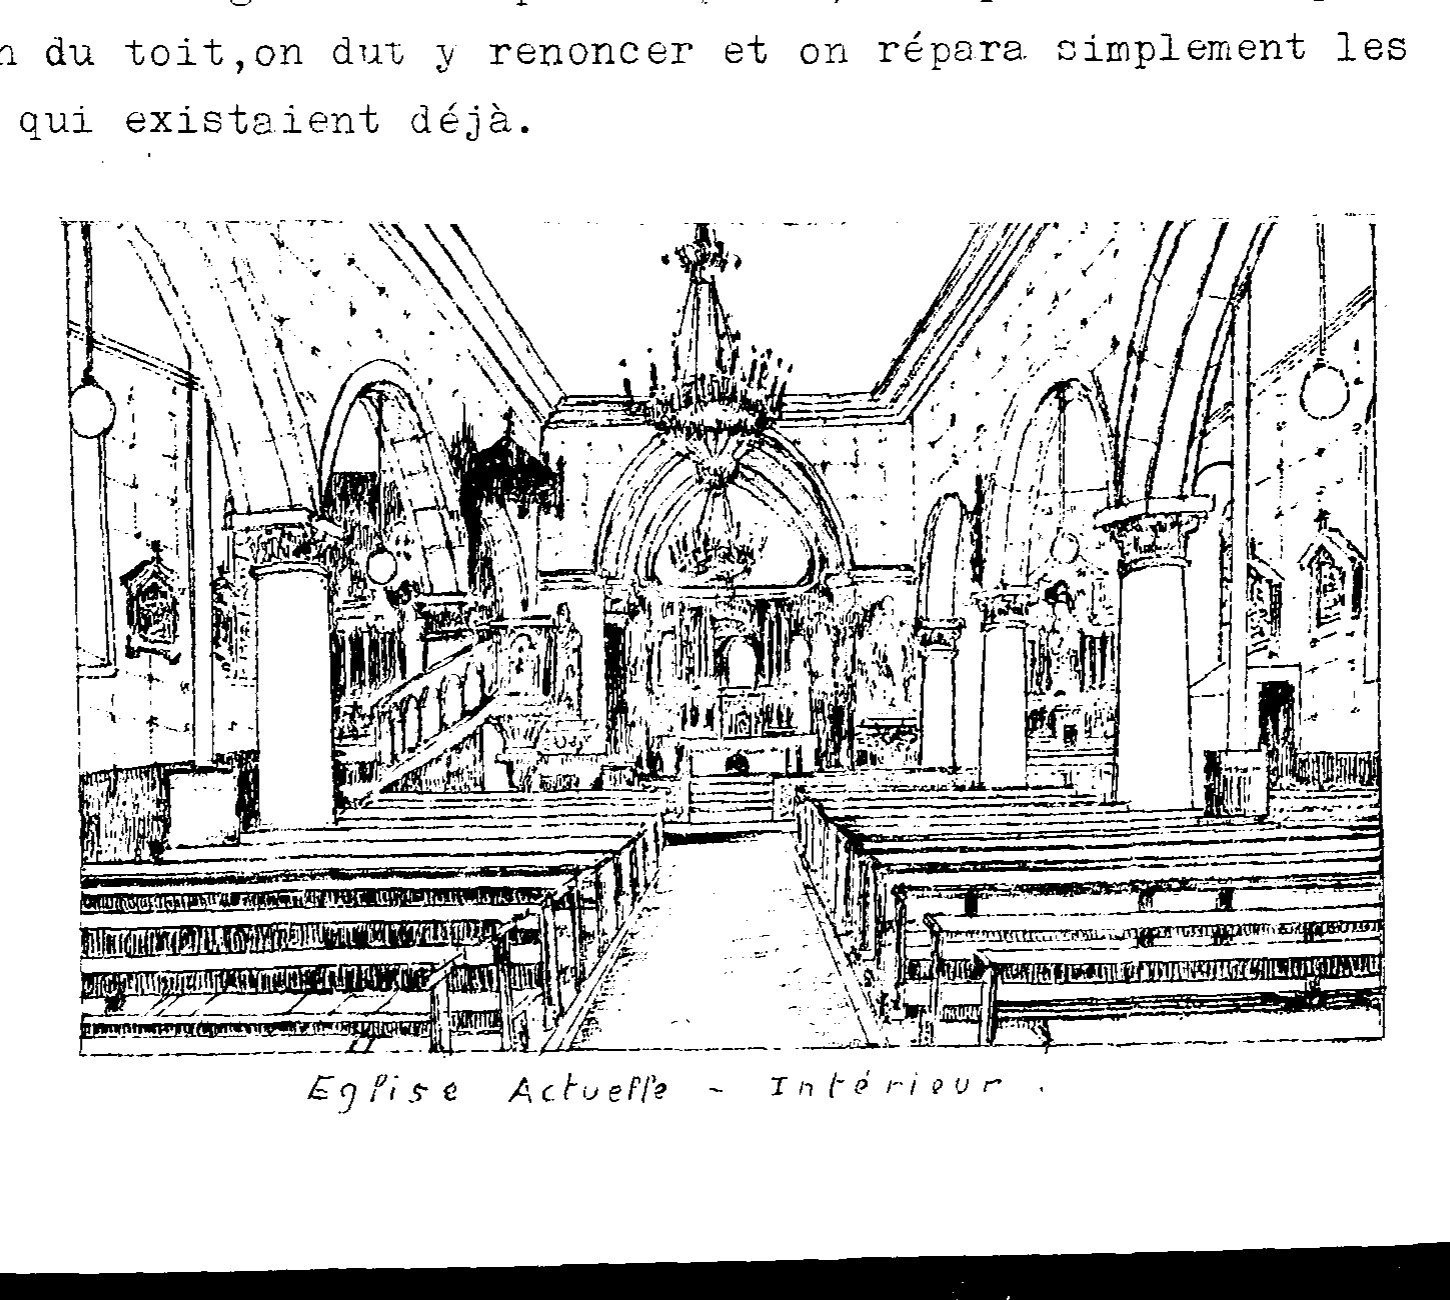
\includegraphics[width=0.62\textwidth]{Illustrations/illus-eglise-interieur.jpg}\end{center}

% --- Page imprimée 204 — vue 207
\begin{center}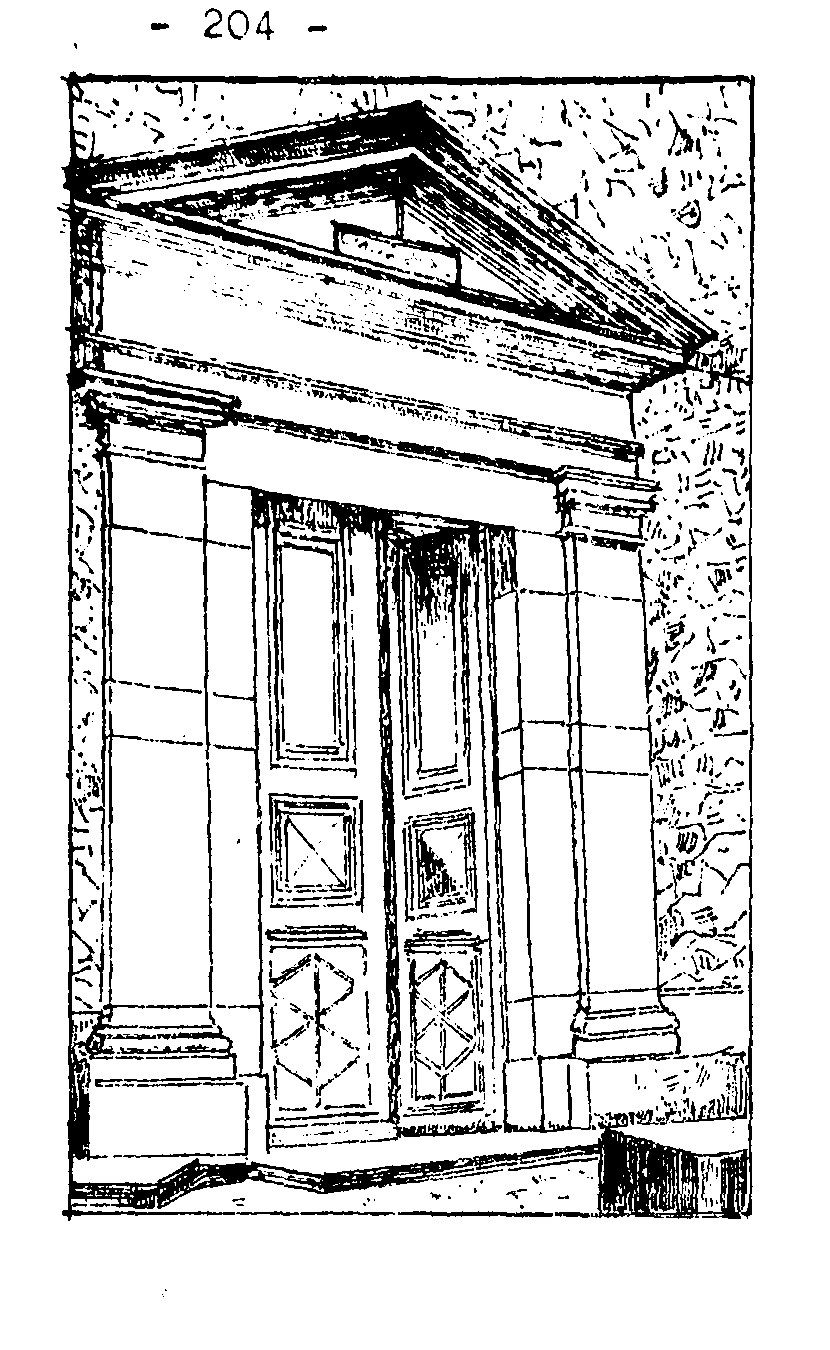
\includegraphics[width=0.62\textwidth]{Illustrations/illus-eglise-exterieur.jpg}\end{center}

En même temps on remplaça la grande porte par celle qui existe actuellement et dont le moindre défaut est d'être d'un style absolument différent de celui de l'église.

Enfin la tour de l'horloge fut transportée sur la façade (page 118). On sait que Mr Guillin avait fait construire cette tour à l'angle sud de la grande porte, près de la galonnière. Mr Pollosse, en un mot, transforma complètement la nef. Il ne conserva que les chapelles de la Ste Vierge et de St-Antoine.

Voici quelques détails sur les chapiteaux des colonnes sculptés par Mr Morétain. Il a voulu faire des chapiteaux romans historiés tout en ne représentant que des sujets religieux. Chaque chapiteau contient quatre scènes séparées entre elles par une feuille grossière ou par des branches d'arbre que la rencontre de l'angle fait recourber en volute.

\begin{center}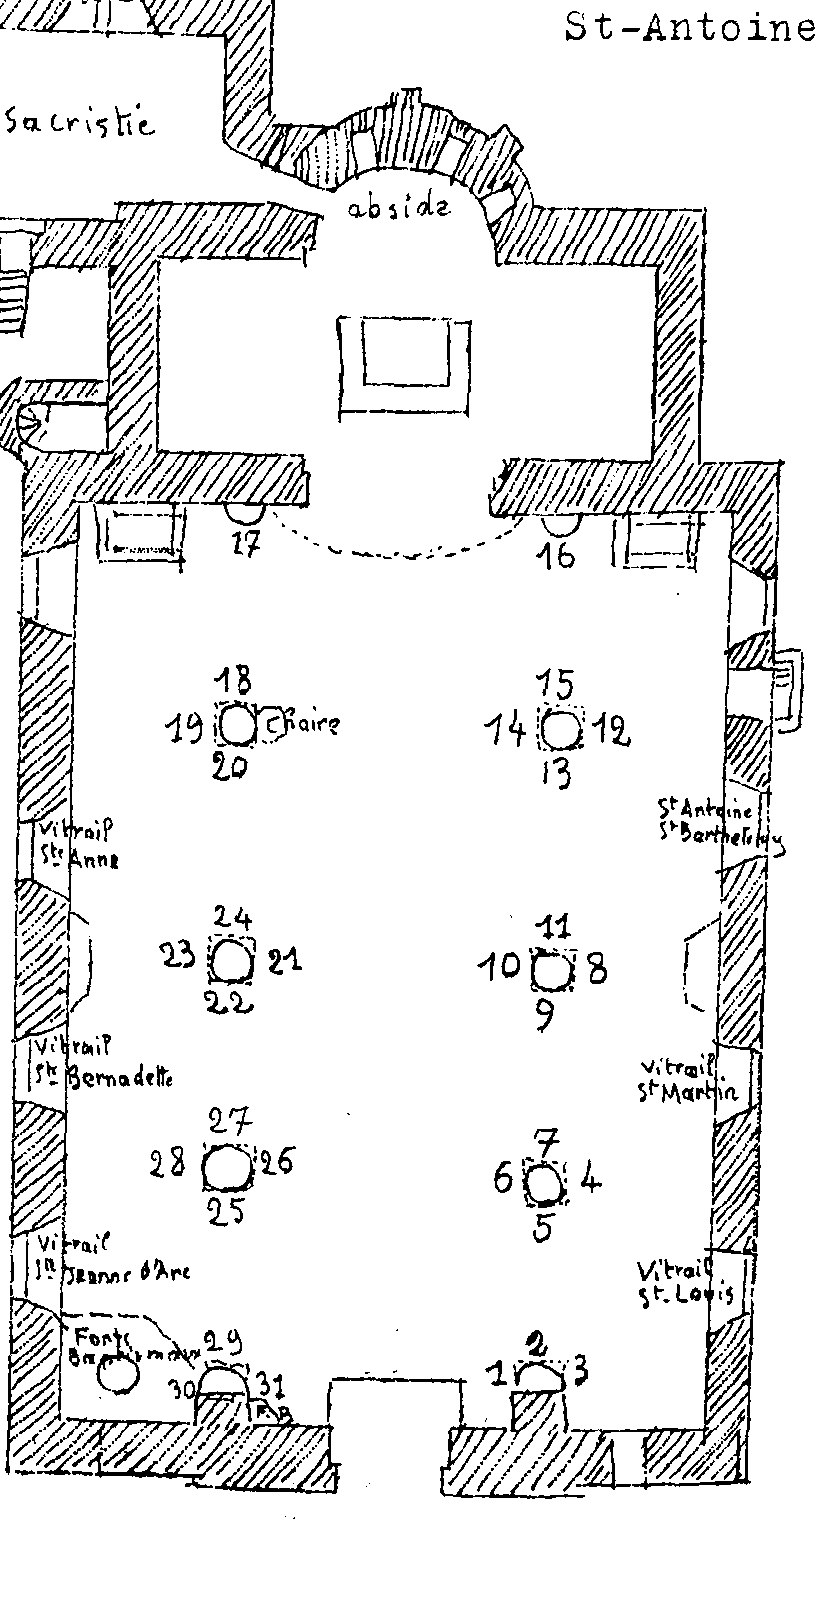
\includegraphics[width=0.62\textwidth]{Illustrations/illus-plan-eglise-actuel.jpg}\end{center}

Ci contre, le plan actuel de l'église avec les numéros d'ordre des tableaux qui vont être décrits.

N. B. — Le plan de l'église a été exécuté au 1/200ème, chaque centimètre représentant 2 mètres.

% --- Page imprimée 205 — vue 208
Sur le chapiteau du pilastre engagé dans le mur de la façade, du côté de l'épître, se trouvent trois tableaux nous représentant des faits bibliques.

Dans le premier, deux hommes nous rappelant les envoyés de Moïse dans la terre de Chanaan pour juger de sa fertilité portent suspendu à un bâton un énorme raisin symbole de l'abondance de grâces que le chrétien vient puiser dans l'église de Dieu.

\begin{center}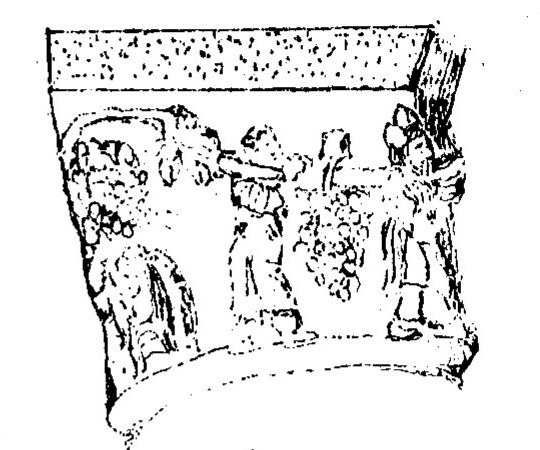
\includegraphics[width=0.28\textwidth]{Illustrations/illus-chapiteau-01.jpg}\end{center}

Dans le second nous voyons le prophète Balaam monté sur son ânesse qui se cabre et se retourne en lui disant : Pourquoi me frappes-tu ? L'ange l'arrête en brandissant un glaive.

\begin{center}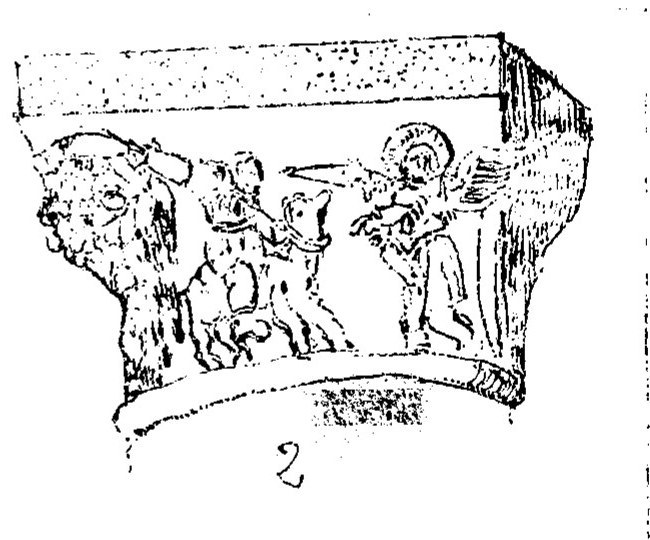
\includegraphics[width=0.28\textwidth]{Illustrations/illus-chapiteau-02.jpg}\end{center}

Le troisième tableau nous offre un épisode de la vie de Tobie. Le jeune homme s'avance suivi de l'Archange Raphael ; ils ont l'un et l'autre le bâton du voyageur. Le chien accourt tout joyeux au devant de son maître.

\begin{center}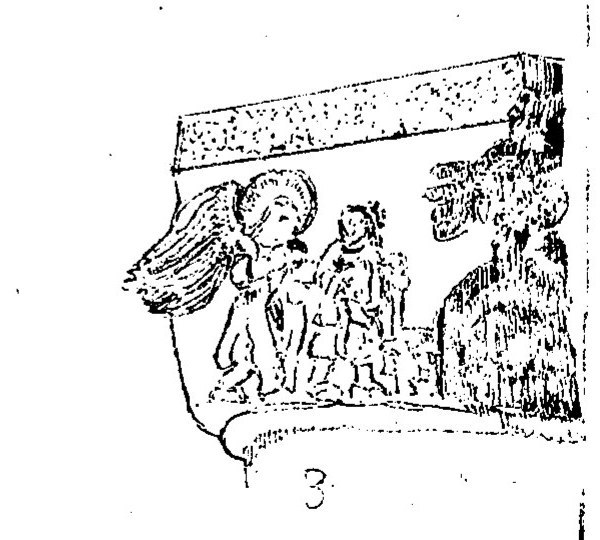
\includegraphics[width=0.28\textwidth]{Illustrations/illus-chapiteau-03.jpg}\end{center}

Les angles du chapiteau sont formés par deux ceps de vigne chargés de raisins et de feuilles.

% --- Page imprimée 206 — vue 209
\begin{center}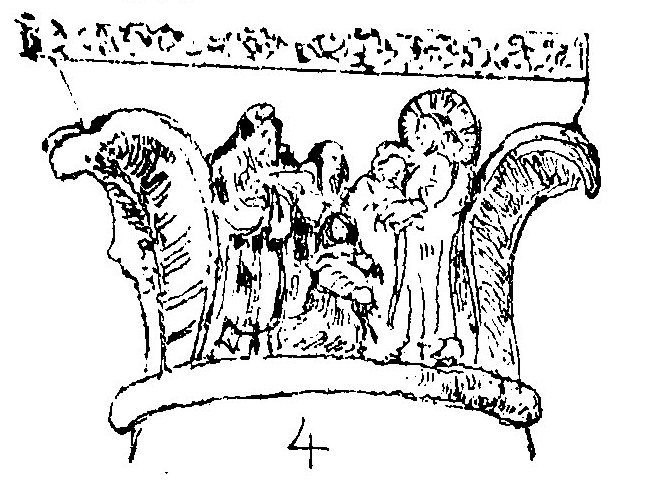
\includegraphics[width=0.28\textwidth]{Illustrations/illus-chapiteau-04.jpg}\end{center}

Les quatre scènes du chapiteau de la première colonne ont trait à la vie de N. S. Jésus-Christ. C'est d'abord la pécheresse, prosternée aux pieds du Divin Maître, qui entend sortir de ses lèvres ces paroles consolantes : « Tes péchés te sont remis ». Trois personnages sont debout auprès de Notre Seigneur.

\begin{center}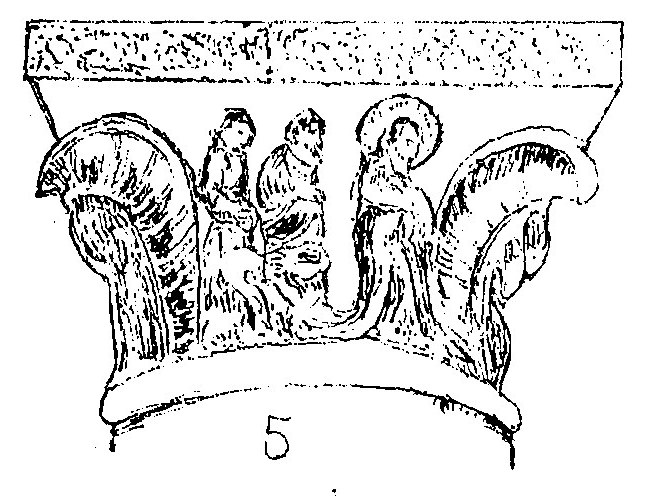
\includegraphics[width=0.28\textwidth]{Illustrations/illus-chapiteau-05.jpg}\end{center}

Vient ensuite le miracle opéré en faveur de l'hémorroïsse. Cette femme baise avec amour le bas de la robe du Sauveur. Une femme et un homme les suivent.

\begin{center}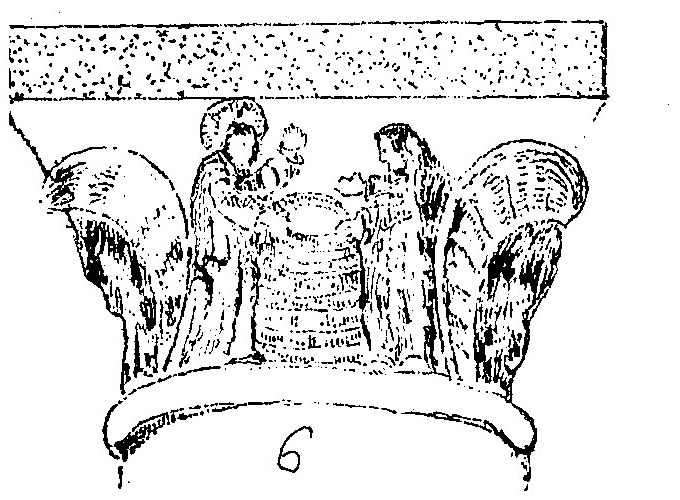
\includegraphics[width=0.28\textwidth]{Illustrations/illus-chapiteau-06.jpg}\end{center}

La troisième scène nous rappelle l'entretien de Notre Seigneur avec la Samaritaine. Ils sont l'un et l'autre debout de chaque côté du puits. La femme, les deux mains appuyées sur la margelle, écoute avec une attention religieuse.

\begin{center}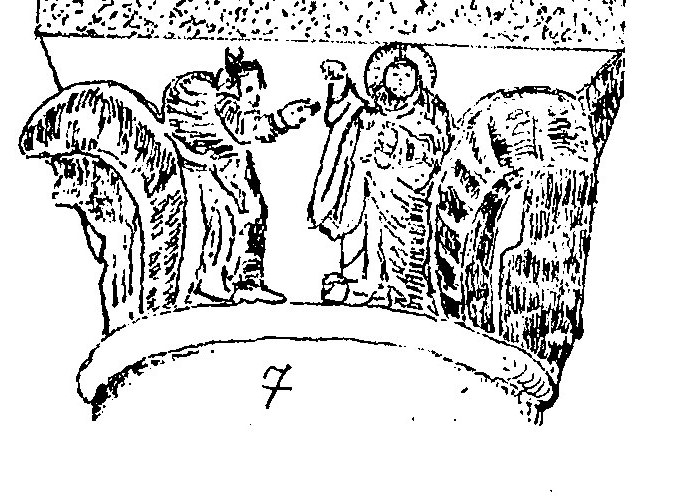
\includegraphics[width=0.28\textwidth]{Illustrations/illus-chapiteau-07.jpg}\end{center}

La quatrième, enfin, nous montre Jésus-Christ au moment de la tentation dans le désert. Le démon lui présente une pierre pour qu'il la change en pain.

Des feuilles de palmiers recourbées à la rencontre de l'angle ornent ce chapiteau.

\begin{center}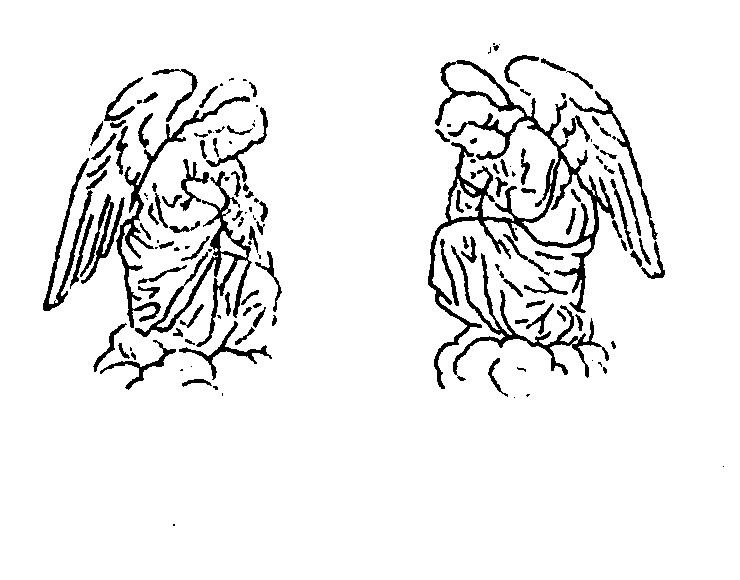
\includegraphics[width=0.28\textwidth]{Illustrations/illus-chapiteau-decor-06.jpg}\end{center}

% --- Page imprimée 207 — vue 210
La seconde colonne est consacrée au souvenir du péché de notre premier père. Nous voyons en premier lieu Adam et Eve assis auprès de Dieu qui leur défend de manger le fruit suspendu sur leurs têtes. Ils étendent, l'un et l'autre, le bras comme pour attester qu'ils seront fidèles à respecter l'ordre de leur Créateur.

\begin{center}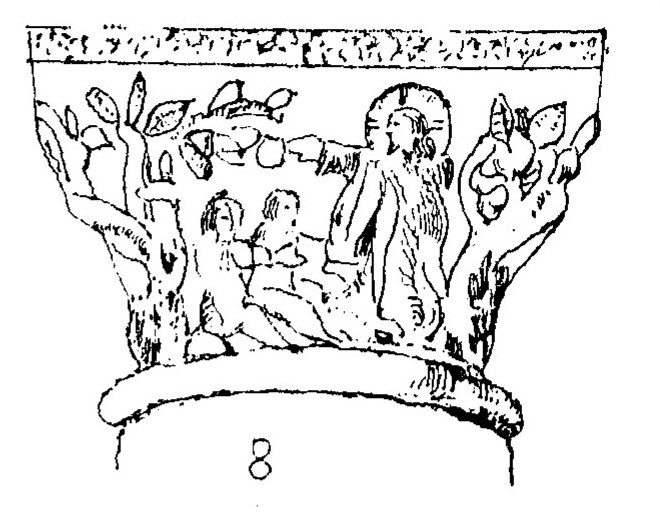
\includegraphics[width=0.28\textwidth]{Illustrations/illus-chapiteau-08.jpg}\end{center}

Néanmoins ils ne peuvent résister au plaisir de goûter le fruit défendu. Le deuxième tableau nous les montre mangeant avec avidité la pomme qu'ils viennent de cueillir.

\begin{center}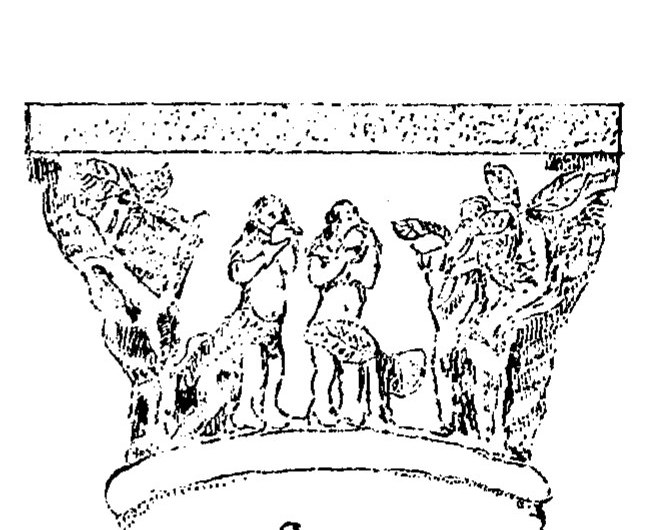
\includegraphics[width=0.28\textwidth]{Illustrations/illus-chapiteau-09.jpg}\end{center}

Au troisième Dieu les appelle. Adam cherche à se cacher derrière un figuier. Eve est auprès de lui. Dieu est debout devant eux.

\begin{center}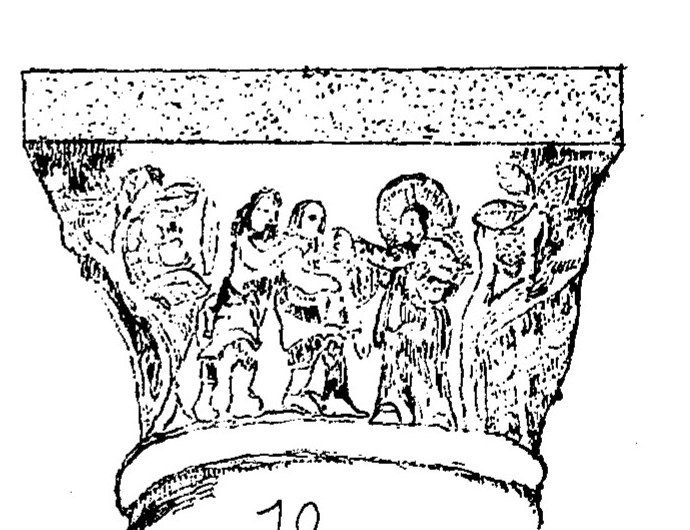
\includegraphics[width=0.28\textwidth]{Illustrations/illus-chapiteau-10.jpg}\end{center}

Enfin sur le quatrième la sentence s'exécute. L'ange armé d'un glaive flamboyant les chasse du paradis terrestre. Eve se lamente, elle sort la première. Adam, au contraire, qui vient de recevoir la promesse du Rédempteur futur, élève les mains et les yeux vers le ciel.

Des pommiers chargés de feuilles et de fruits forment les angles du chapiteau.

\begin{center}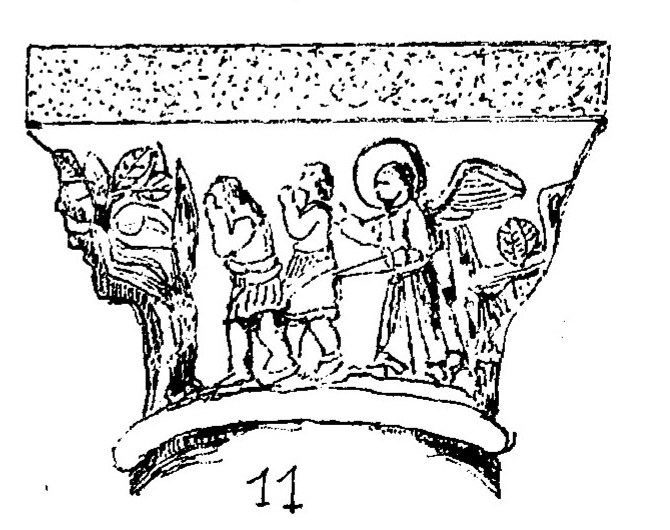
\includegraphics[width=0.28\textwidth]{Illustrations/illus-chapiteau-11.jpg}\end{center}

% --- Page imprimée 208 — vue 211
Sur la troisième colonne se déroulent les mystères de l'Incarnation et de l'enfance de Notre-Seigneur Jésus-Christ.

L'archange descend du ciel et annonce à Marie qu'elle est appelée à devenir la mère de Dieu. Elle se retourne à la parole de l'envoyé céleste ; par son geste elle indique qu'elle donne son consentement. Elle a devant elle le lis, symbole de la virginité.

\begin{center}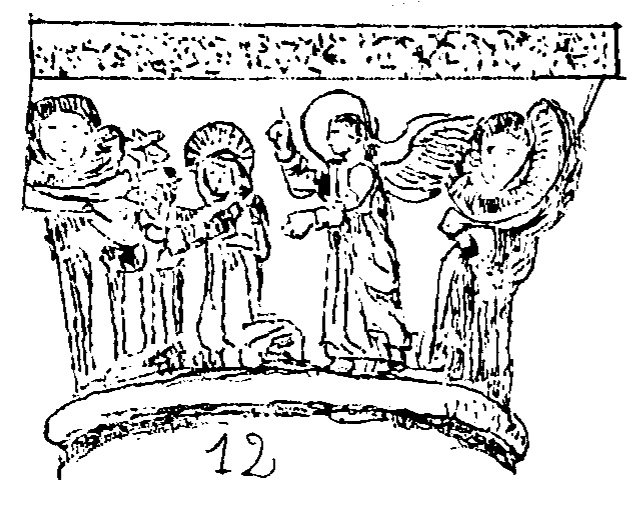
\includegraphics[width=0.28\textwidth]{Illustrations/illus-chapiteau-12.jpg}\end{center}

Vient ensuite l'adoration des bergers. L'enfant Jésus est couché dans la crèche. Marie est à genoux près de lui dans la contemplation. St-Joseph est debout derrière elle. Trois bergers appuyés sur leur houlette offrent à l'Enfant leurs hommages.

\begin{center}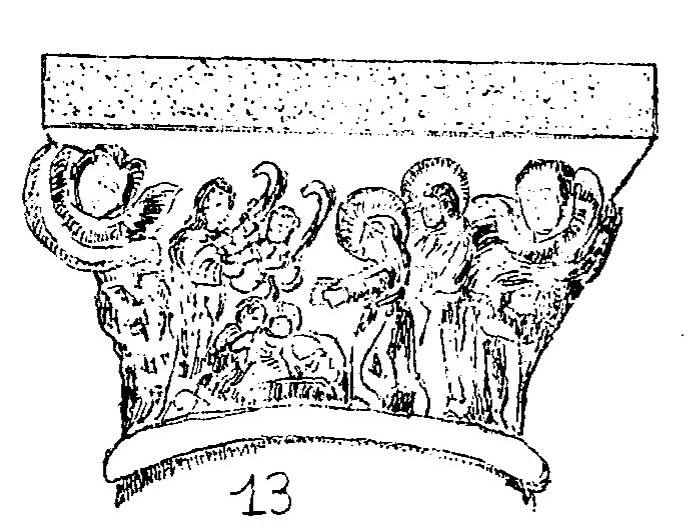
\includegraphics[width=0.28\textwidth]{Illustrations/illus-chapiteau-13.jpg}\end{center}

Plus loin, l'adoration des Mages. Marie tient l'Enfant-Dieu entre ses bras. L'un des Mages, à genoux lui offre son présent ; les deux autres sont debout derrière lui. Ils ont sur la tête la couronne royale. St-Joseph sous la figure d'un vieillard est dans l'étonnement à la vue de tout ce qui s'accomplit sous ses yeux.

\begin{center}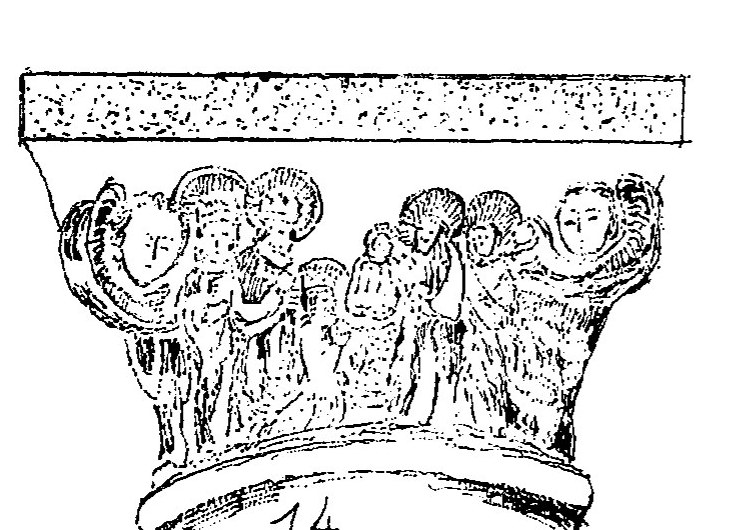
\includegraphics[width=0.28\textwidth]{Illustrations/illus-chapiteau-14.jpg}\end{center}

Vient ensuite le mystère de la Présentation. Marie donne l'Enfant au vieillard Siméon qui est près de l'autel en costume de grand prêtre. Il a à ses côtés la prophétesse Anne. St-Joseph est auprès de Marie. Deux têtes d'anges accouplées séparent les tableaux.

\begin{center}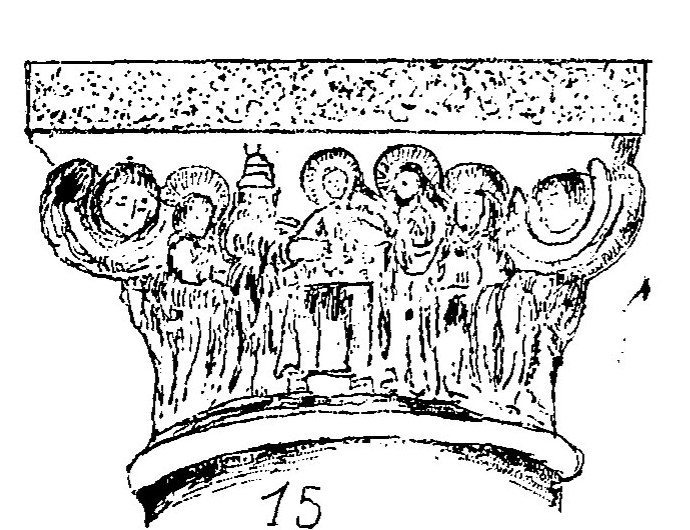
\includegraphics[width=0.28\textwidth]{Illustrations/illus-chapiteau-15.jpg}\end{center}

% --- Page imprimée 209 — vue 212
Sur la demi-colonne engagée dans le mur de la chapelle Saint-Antoine, Mr Moretain a représenté la mort du saint ermite. Il est couché, la tête appuyée sur une pierre et tenant un crucifix entre ses mains. Deux moines, debout, auprès de lui pleurent ; un autre soutient la tête du mourant ; un quatrième, à genoux à ses pieds, l'asperge d'eau bénite avec un énorme goupillon, tandis que deux autres lisent les prières des agonisants. Près de St-Antoine se trouve le père traditionnel. Une colombe, image de l'âme du saint, prend son vol vers les cieux.

Aux angles du chapiteau sont deux anges : l'un d'eux montre le ciel ; l'autre tient dans ses mains une couronne.

\begin{center}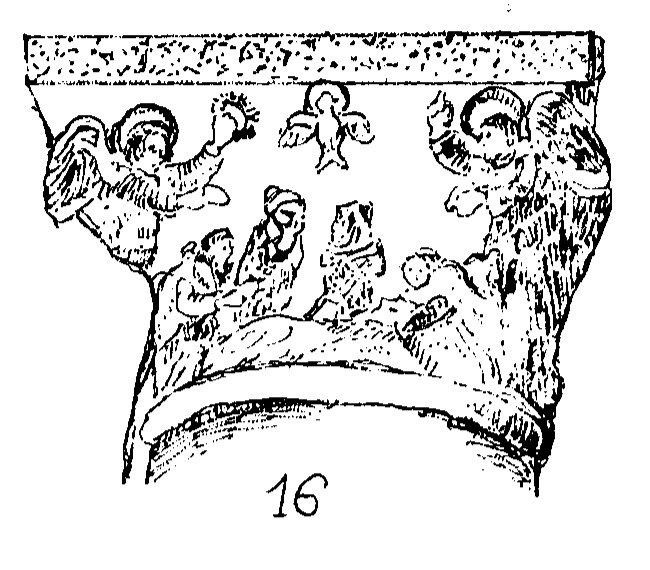
\includegraphics[width=0.28\textwidth]{Illustrations/illus-chapiteau-16.jpg}\end{center}

Du côté de l'Evangile, sur la demi-colonne de la chapelle de la Sainte Vierge, Marie est debout au milieu de deux anges qui la vénèrent ; leurs ailes forment l'angle du chapiteau.

La scène représente l'exaltation de Marie au-dessus de toute créature. De chaque côté, deux personnages nimbés dont il m'est impossible de définir le caractère.

A droite une femme montre le ciel  
à gauche une religieuse ; le voile baissé, presse avec amour une croix nue.

\begin{center}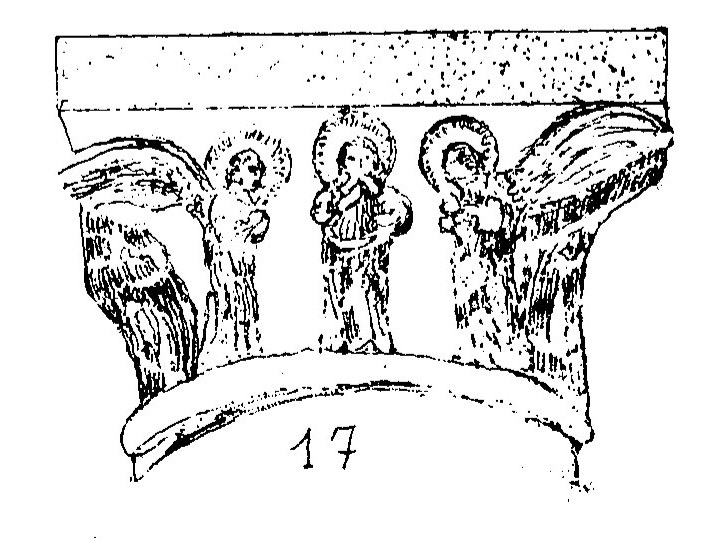
\includegraphics[width=0.28\textwidth]{Illustrations/illus-chapiteau-17.jpg}\end{center}

% --- Page imprimée 210 — vue 213
Sur la colonne de la chaire ont été figurées trois circonstances particulières de la vie de Notre-Seigneur.

D'un côté, son Baptême par St-Jean Baptiste. Le Sauveur du monde est à genoux devant le Précurseur qui verse de l'eau sur la tête du Messie. Deux disciples assistent au mystère. Le Saint-Esprit, en forme de colombe, descend sur Jésus-Christ.

\begin{center}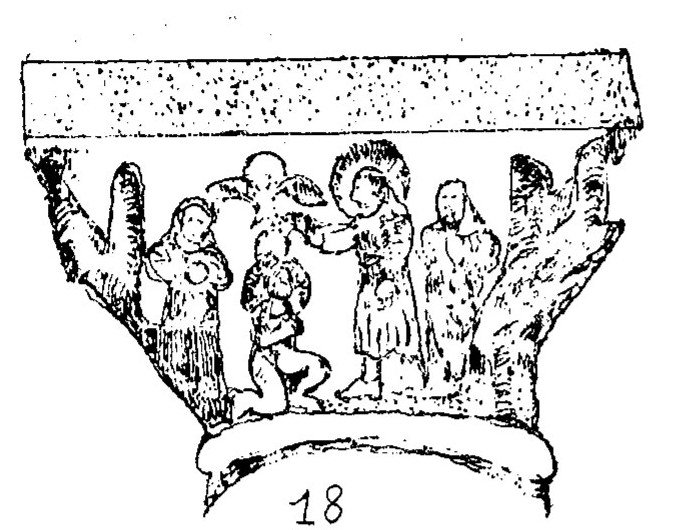
\includegraphics[width=0.28\textwidth]{Illustrations/illus-chapiteau-18.jpg}\end{center}

De l'autre côté, la vocation de Zachée. Le chef des Pharisiens qui ne peut voir Jésus à cause de la foule est monté sur un arbre qui forme précisément l'angle du chapiteau. Quatre disciples accompagnent le Sauveur qui s'entretient avec Zachée.

\begin{center}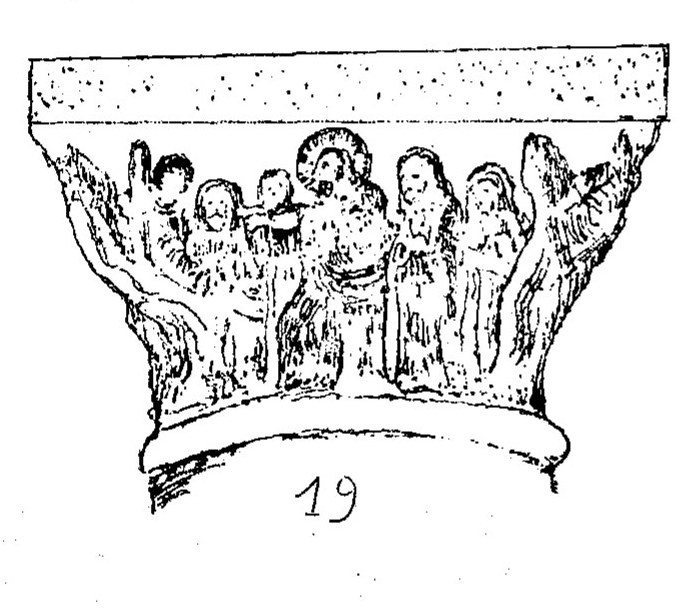
\includegraphics[width=0.28\textwidth]{Illustrations/illus-chapiteau-19.jpg}\end{center}

Enfin le troisième tableau nous montre Jésus-Christ prêchant sa doctrine dans les villes de Judée. Deux apôtres sont debout, devant lui ; trois femmes dont deux assises sont également à ses côtés.

Ici encore deux arbres forment l'angle du chapiteau ; sur l'un se trouvent deux personnages qui écoutent le Divin Maître ; sur l'autre il n'y en a qu'un seul.

\begin{center}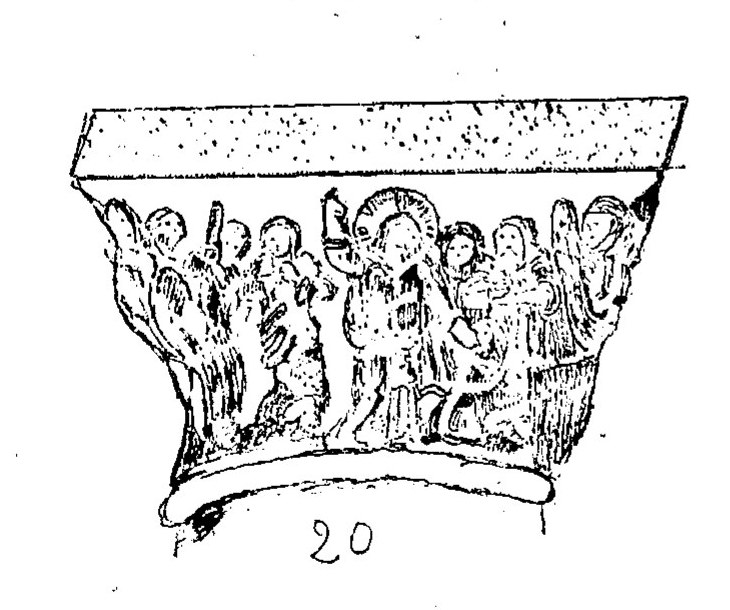
\includegraphics[width=0.28\textwidth]{Illustrations/illus-chapiteau-20.jpg}\end{center}

% --- Page imprimée 211 — vue 214
La colonne suivante est consacrée au sacrifice d'Abraham.

Dieu ordonne au saint patriarche d'immoler son fils Isaac. Abraham à genoux devant Dieu promet d'exécuter ses ordres. Isaac est dans un plan éloigné.

\begin{center}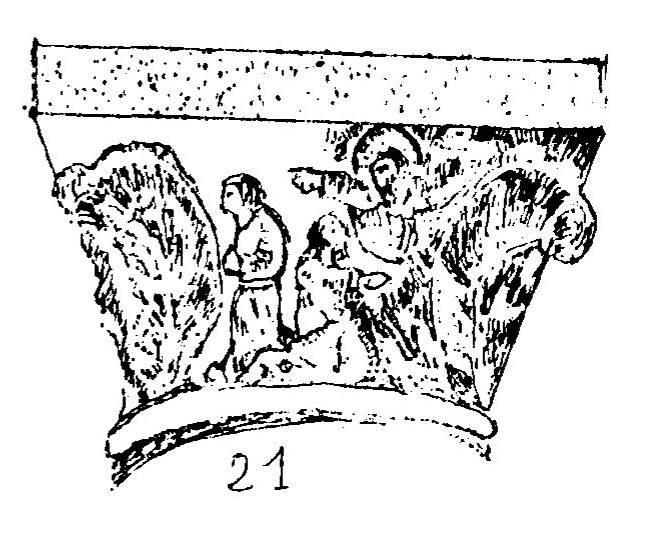
\includegraphics[width=0.28\textwidth]{Illustrations/illus-chapiteau-21.jpg}\end{center}

Nous voyons ensuite ces deux saints personnages gravissant la montagne du sacrifice. Isaac porte le bois ; Abraham le suit, une torche et un glaive à la main.

\begin{center}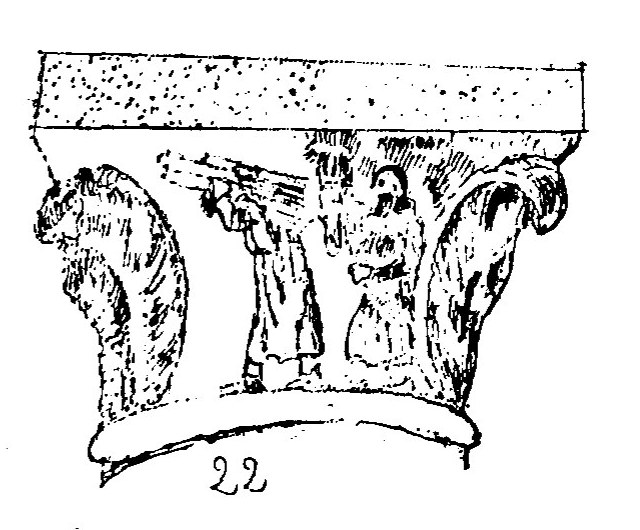
\includegraphics[width=0.28\textwidth]{Illustrations/illus-chapiteau-22.jpg}\end{center}

Ils arrivent enfin au lieu où doit s'accomplir l'immolation ; Isaac est étendu sur le bûcher et Abraham se dispose à l'égorger lorsqu'un ange, descendant du ciel, arrête son bras.

\begin{center}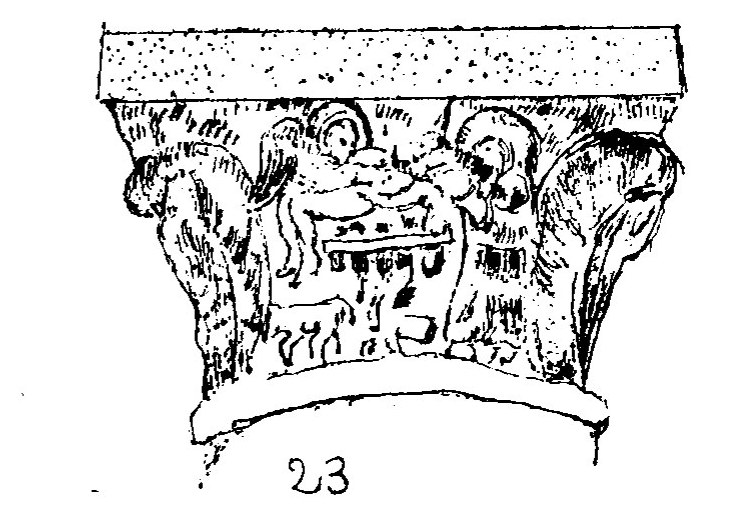
\includegraphics[width=0.28\textwidth]{Illustrations/illus-chapiteau-23.jpg}\end{center}

Dans la quatrième scène, Abraham et Isaac, placés de chaque côté du bûcher, disposent pour le sacrifice le bélier qui est venu providentiellement s'offrir comme victime.

\begin{center}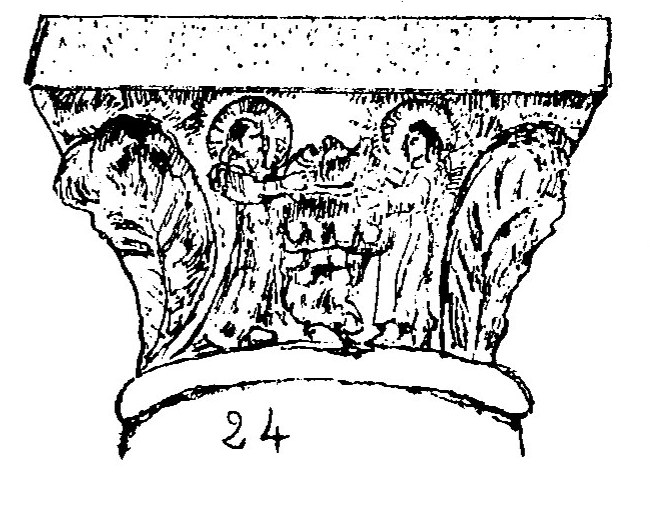
\includegraphics[width=0.28\textwidth]{Illustrations/illus-chapiteau-24.jpg}\end{center}

% --- Page imprimée 212 — vue 215
\begin{center}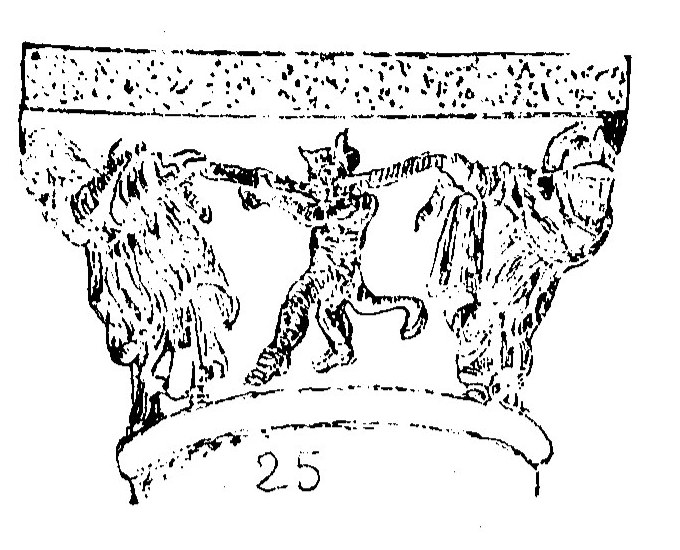
\includegraphics[width=0.28\textwidth]{Illustrations/illus-chapiteau-25.jpg}\end{center}

\begin{center}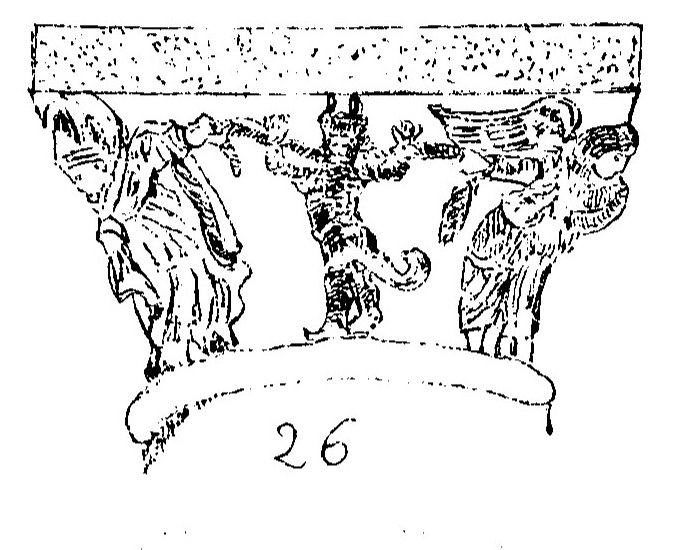
\includegraphics[width=0.28\textwidth]{Illustrations/illus-chapiteau-26.jpg}\end{center}

\begin{center}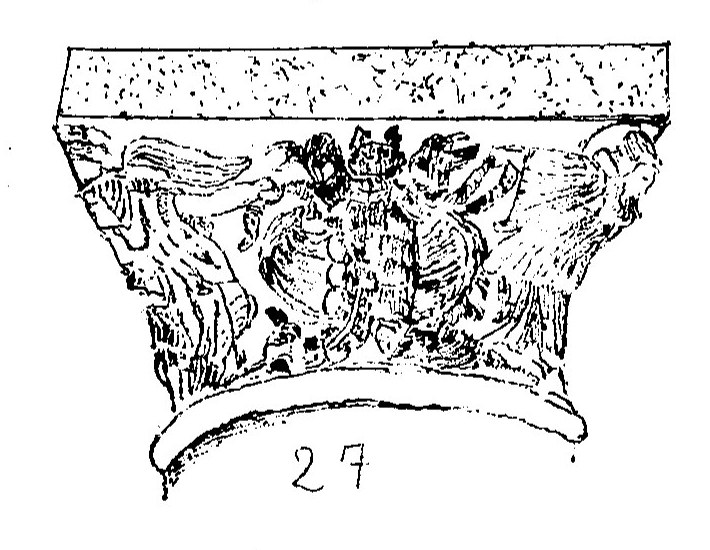
\includegraphics[width=0.28\textwidth]{Illustrations/illus-chapiteau-27.jpg}\end{center}

\begin{center}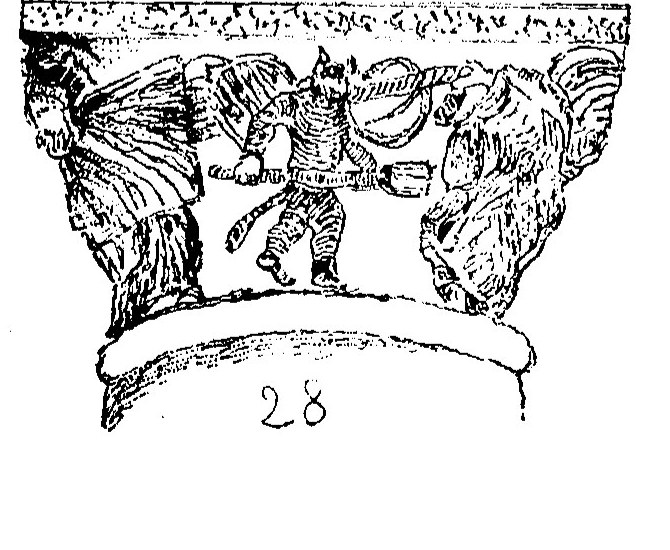
\includegraphics[width=0.28\textwidth]{Illustrations/illus-chapiteau-28.jpg}\end{center}

Le sixième chapiteau nous représente un sujet curieusement traité. On peut l'intituler : le triomphe de la hiérarchie ecclésiastique sur la hiérarchie diabolique.

Aux quatre angles sont : un ange, les ailes déployées ; le souverain Pontife, la tête surmontée de la tiare ; l'Évêque avec sa mitre ; le Prêtre revêtu du surplis et de la barrette. Ils tirent fortement une corde qui enlace le corps du démon représenté successivement sur les quatre faces du chapiteau et chaque fois avec des symboles particuliers, tantôt grimaçant d'une manière effrayante, tantôt menaçant ses ennemis avec un énorme trident.

% --- Page imprimée 213 — vue 216
Enfin, sur le pilastre des Fonts Baptismaux nous voyons d'abord un ange, les ailes étendues et dans la posture de l'adoration et du respect.

À droite l'image de Notre-Seigneur Jésus-Christ sous la figure du Bon Pasteur rapportant sur ses épaules la brebis égarée.

À gauche Moïse tient entre ses mains les Tables de la Loi.

Deux énormes feuilles de palmiers en complètent l'ornementation.

\begin{center}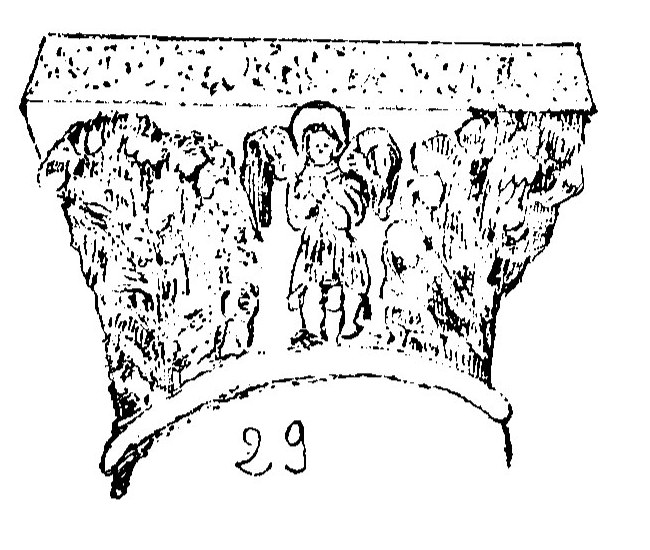
\includegraphics[width=0.28\textwidth]{Illustrations/illus-chapiteau-29.jpg}\end{center}

\begin{center}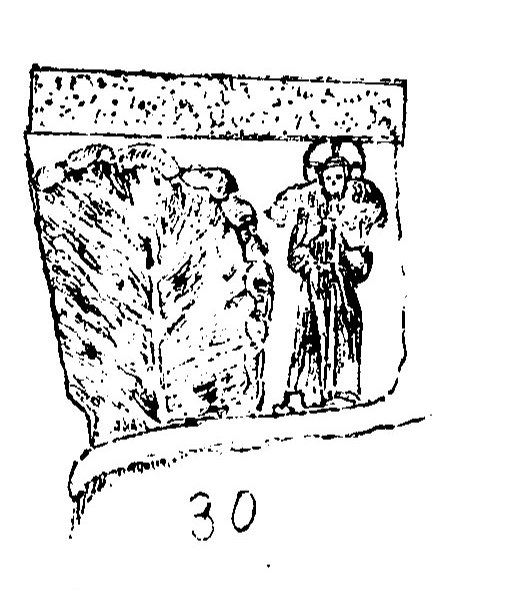
\includegraphics[width=0.28\textwidth]{Illustrations/illus-chapiteau-30.jpg}\end{center}

\begin{center}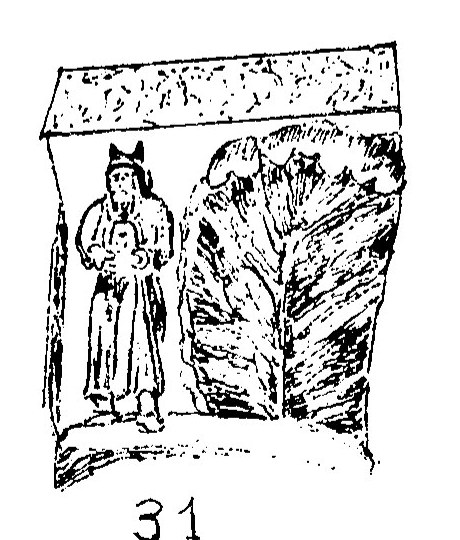
\includegraphics[width=0.28\textwidth]{Illustrations/illus-chapiteau-31.jpg}\end{center}

Telle est l'œuvre de Mr Morétain. L'exécution en est imparfaite, grossière même si l'on veut ; il y a dans le groupement des personnages bien des positions défectueuses, parfois des vides trop considérables ; mais l'idée plaît et rachète par son originalité ce qui a pu manquer à l'exécution. Du reste les heures dont Mr Morétain pouvait disposer étaient comptées et surtout la pierre qu'il voulait faire parler aux yeux des fidèles ne se pliait que très difficilement aux inspirations de l'artiste.

% --- Page imprimée 214 — vue 217
Il était réservé à Mr Bouteille de donner à notre église ce cachet artistique qui se manifeste surtout dans le choeur, en réparant autant qu'il était possible les mutilations qu'elle avait eu à subir dans le cours des siècles. Il nous reste à énumérer brièvement tout ce qu'il fit pendant les 22 années qu'il administra notre paroisse.

\begin{center}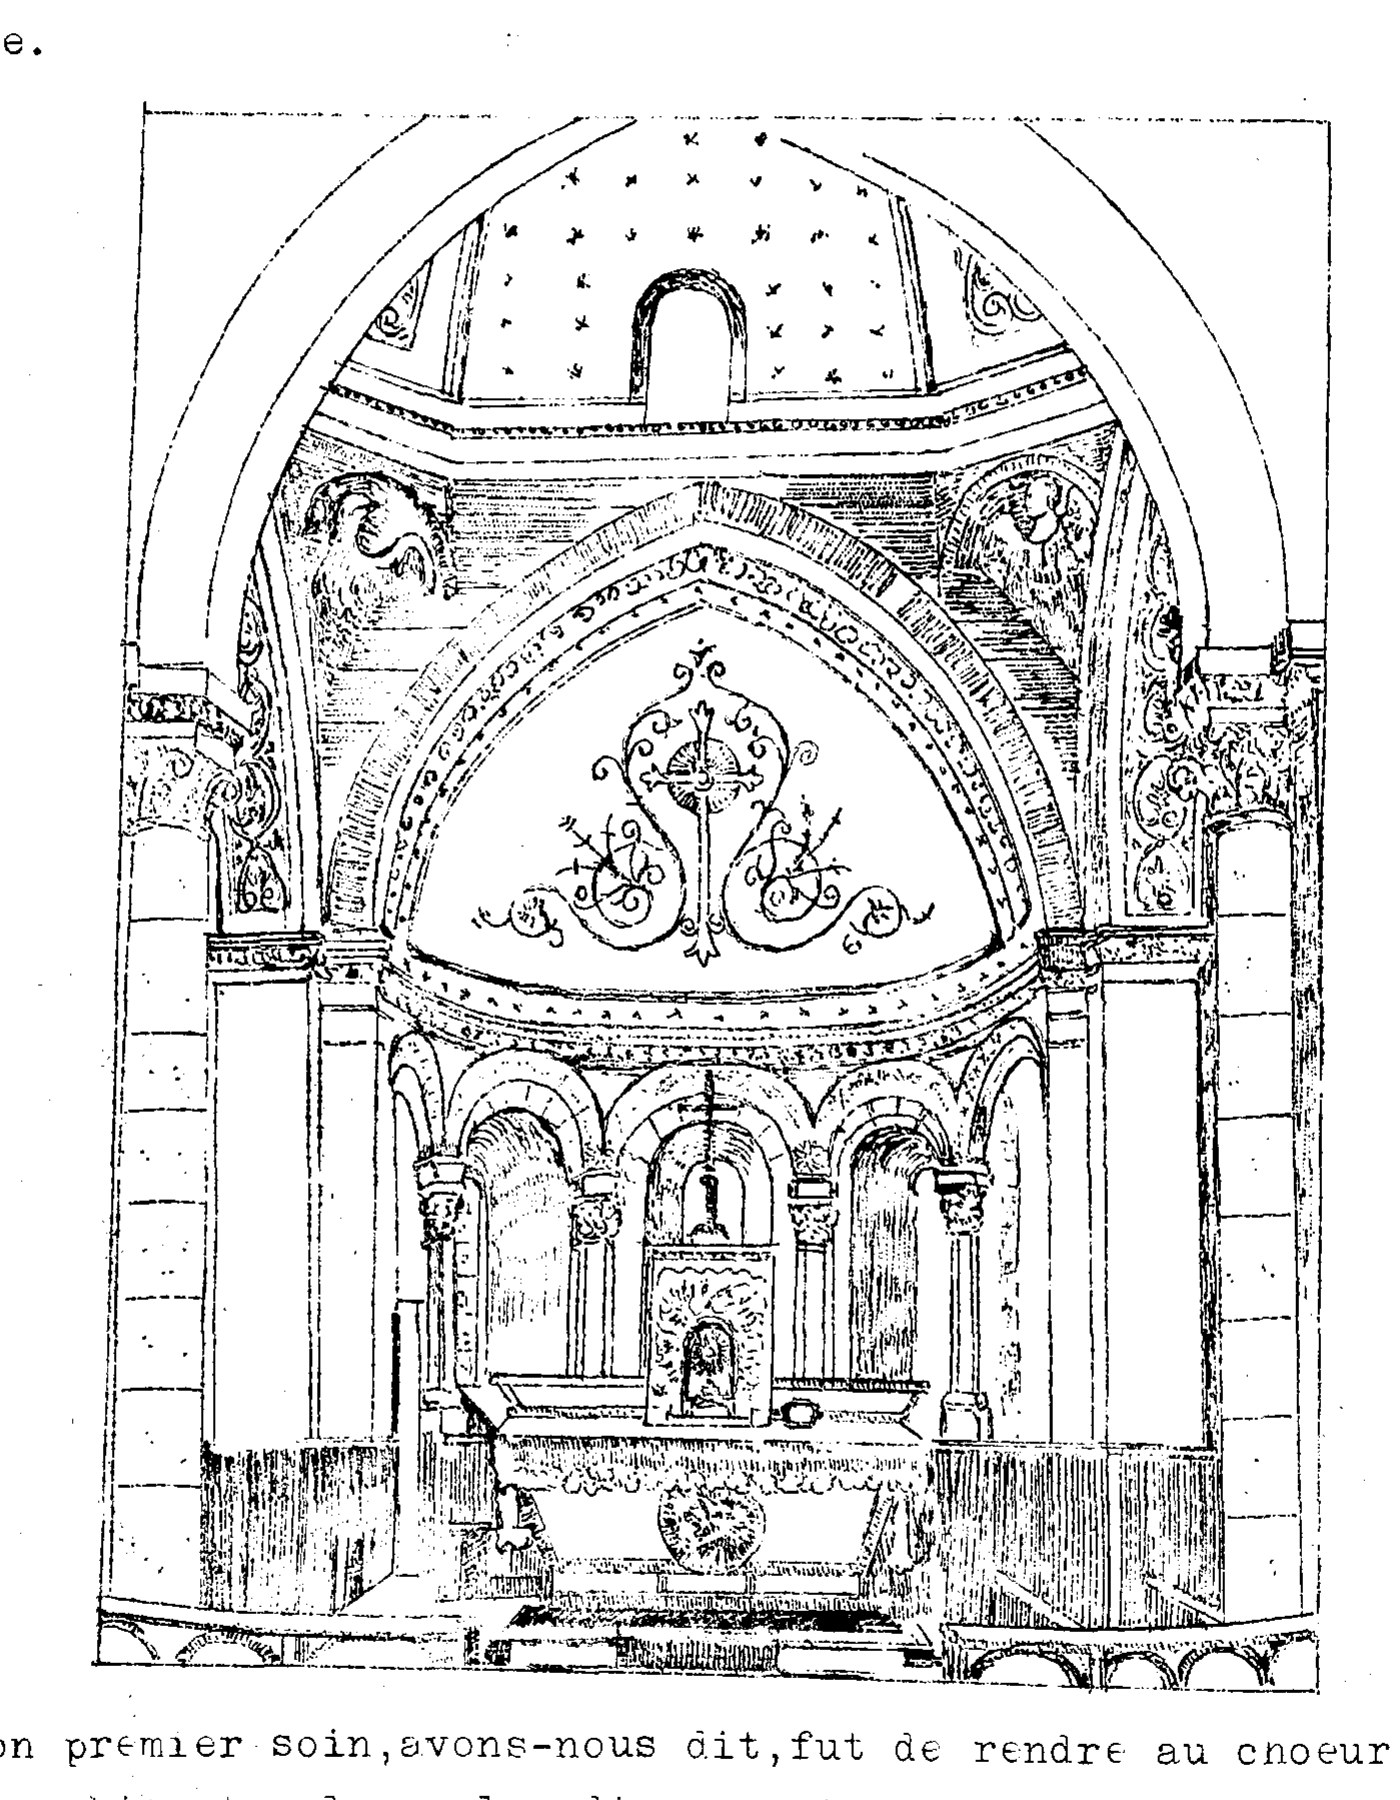
\includegraphics[width=0.62\textwidth]{Illustrations/illus-chapiteau-decor-31.jpg}\end{center}

Son premier soin, avons-nous dit, fut de rendre au choeur le caractère architectural que les diverses transformations avaient presque complètement fait disparaître. Il fit appel pour cela aux conseils et à la longue expérience d'un architecte Lyonnais, Mr Bresson, qui venait de construire le château de Gros-Bois et restaurer Lacarelle

% --- Page imprimée 215 — vue 218
Il fut facile de déterminer la forme primitive de l'abside ; les églises de la contrée auraient pu servir, au besoin, de modèles. On dégagea les trois fenêtres qui avaient été murées. On refit, en ciment, la corniche et les pilastres qui avaient disparu. Le sanctuaire blanchi à la chaux fut orné de peintures qui font ressortir davantage la pureté des lignes et donnent au choeur un aspect régulier et gracieux. Les voûtes du transept et la coupole sont parsemées d'étoiles d'or sur fond d'azur ; dans les pendentifs sont représentés les quatre animaux symboliques des Evangélistes. Ces réparations furent exécutées en 1864. La même année il fit reconstruire la sacristie et remplacer le vieil autel en bois de St-Antoine par un autel en pierre. En 1867 il faisait exécuter, d'après les plans de Bresson, celui de la Sainte-Vierge.

Ce fut vers cette époque, sans doute, qu'il découvrit dans l'embrasure d'une fenêtre, chez les religieuses, une antique statue de la Sainte-Vierge que de graves mutilations avaient forcé Mr Guillin de remplacer. Cette statue, envoyée à Lyon, fut réparée et placée sur l'autel. C'est une vierge à la rose qui offre un certain cachet d'antiquité. Marie tient l'enfant Jésus qui porte lui-même, dans la main gauche, le monde surmonté d'une croix ; elle lui offre de la main droite une rose. Les deux figures sont d'une naïveté charmante.

Nous voyons au musée de Lyon une Vierge du XIIème siècle représentant le même sujet. Les vêtements amples et à plis nombreux de celle de notre église ne permettent pas, sans doute, de la faire remonter à cette époque.

\begin{center}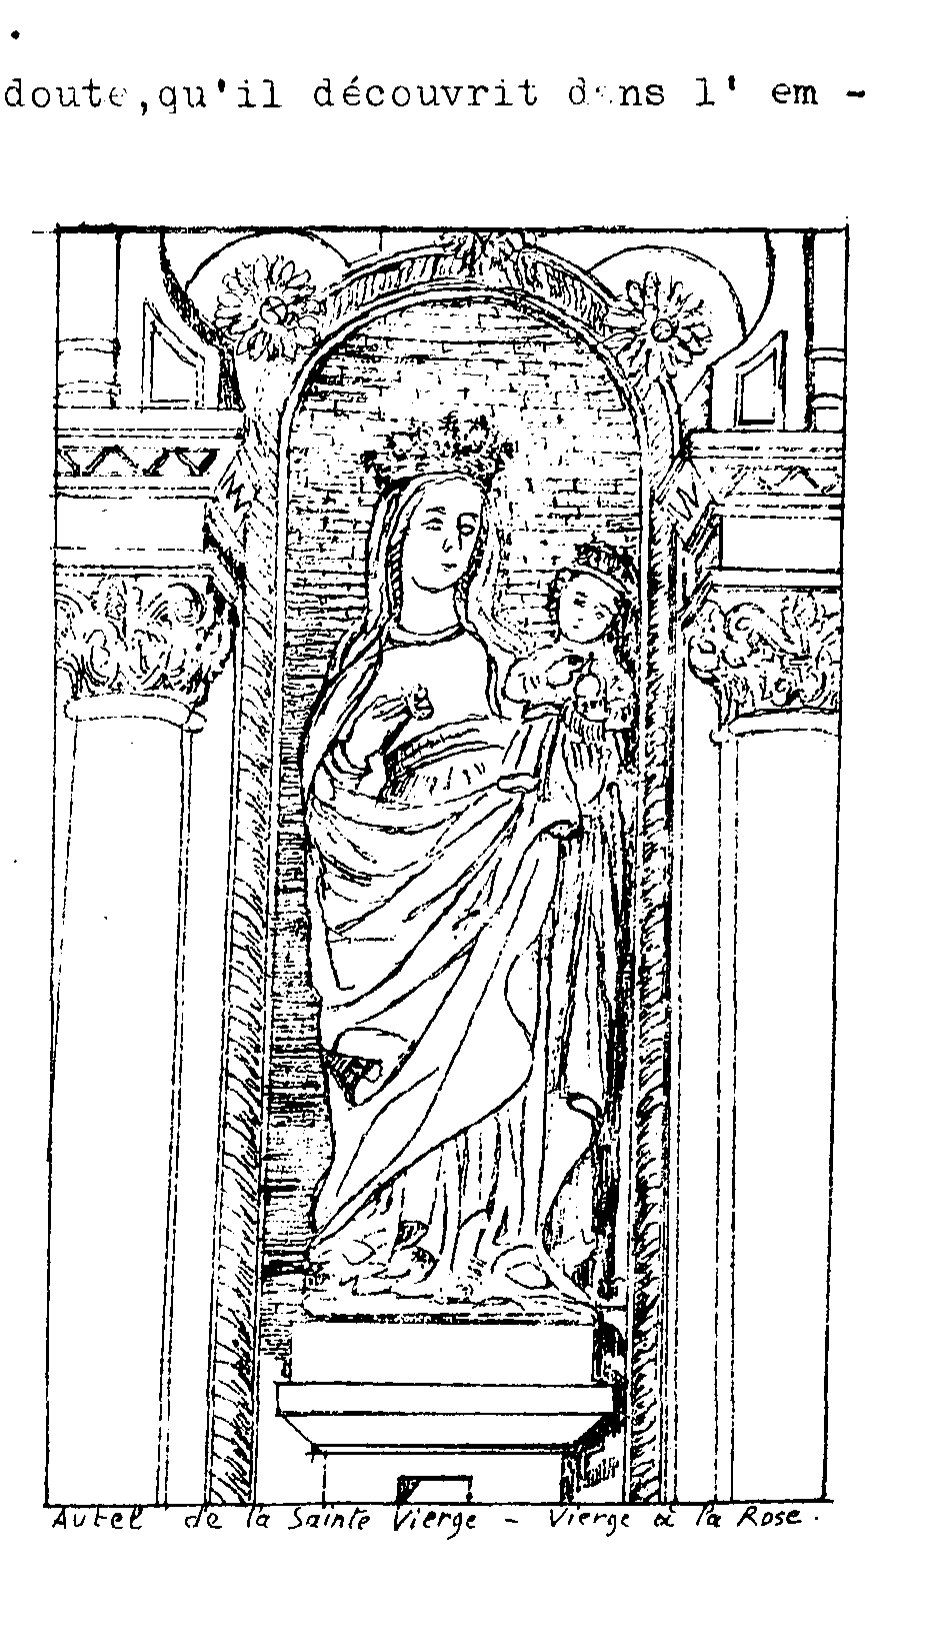
\includegraphics[width=0.62\textwidth]{Illustrations/illus-autel-vierge-rose.jpg}\end{center}
% --- Page imprimée 216 — vue 219 (suite)
faire remonter à cette époque. Aucun titre, au reste, ne nous indique à quel moment elle fut achetée ; peut-être remonte-t-elle à la fondation même de la chapelle des Testenoire qui portait le nom de N.D. de Gré ou Grez.

Mr Bouteille remplaçait en même temps la statue en bois de St-Antoine par une statue en pierre qu'il fit sculpter à Lyon. Cette même année Mr Bernard, menuisier à Lyon fit les boiseries du choeur.

En 1872 il fit placer aux fenêtres de l'église des vitraux sortant des ateliers de Mme Vve Pagnon à Lyon. Ceux de l'abside renferment chacun trois médaillons représentant quelques-uns de nos mystères. Celui de droite nous offre le mystère de l'Annonciation, de la naissance de Notre Seigneur et de son Baptême ; celui du milieu la Cène, la mort de N.S. et sa résurrection ; celui de gauche : la collation des clefs à St-Pierre, l'Ascension et la Pentecôte. On a donné aux divers personnages le type de la période romane pour les harmoniser avec le style du choeur. Les vitraux ont coûté 1745 frs. Ils ont été payés avec l'argent des confréries.

La fenêtre ogivale de Gorze qui a été conservée a, elle aussi, reçu un vitrail à deux personnages : St-Antoine et St-Barthelemy qui sont séparés par le meneau.

Les lustres romans furent placés, deux en 1873, les deux autres en 1875. Ils sortent des ateliers de Mr Capillery fondeur à Lyon ainsi que les beaux chandeliers achetés la même année au prix de 600 francs.

La Fabrique fit en même temps sculpter les Fonts nouveaux actuels
% --- Page imprimée 217 — vue 220 (suite)
par Mr Labrosse, menuisier à Gibles, qui ont coûté 110 frs.

Le même artiste devait en 1877 exécuter la chaire dans le même style. Elle est en bois de chêne, comme les confessionnaux. Les sculptures des chapiteaux sont faites avec soin, les cinq pans ornés de statuettes en pied. Celle du milieu représente le bon Pasteur avec la houlette et portant sur ses bras la brebis égarée. Les quatre autres figurent les quatre évangélistes accompagnés de leurs animaux symboliques (voir gravure page suivante). La chaire a coûté 1500 frs

L'ancienne qui n'avait aucune valeur a été placée dans la nouvelle église du Vieux Château, paroisse démembrée de celle de Cenves.

Les fonts baptismaux (qui tiennent lieu actuellement de placard),

\begin{center}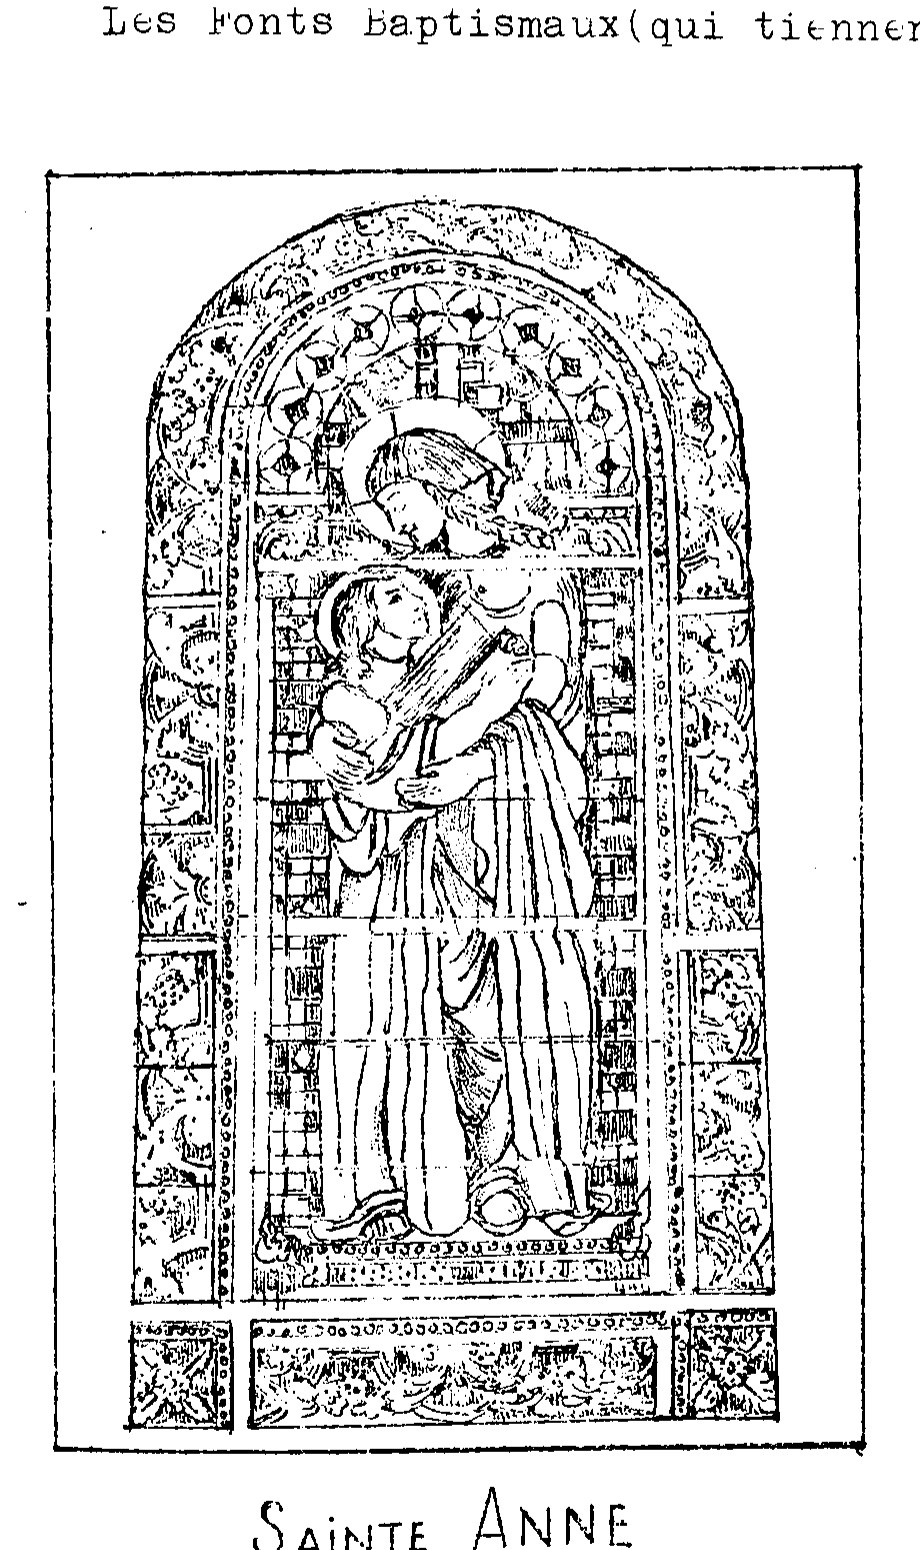
\includegraphics[width=0.62\textwidth]{Illustrations/illus-sainte-anne.jpg}\end{center}

\begin{center}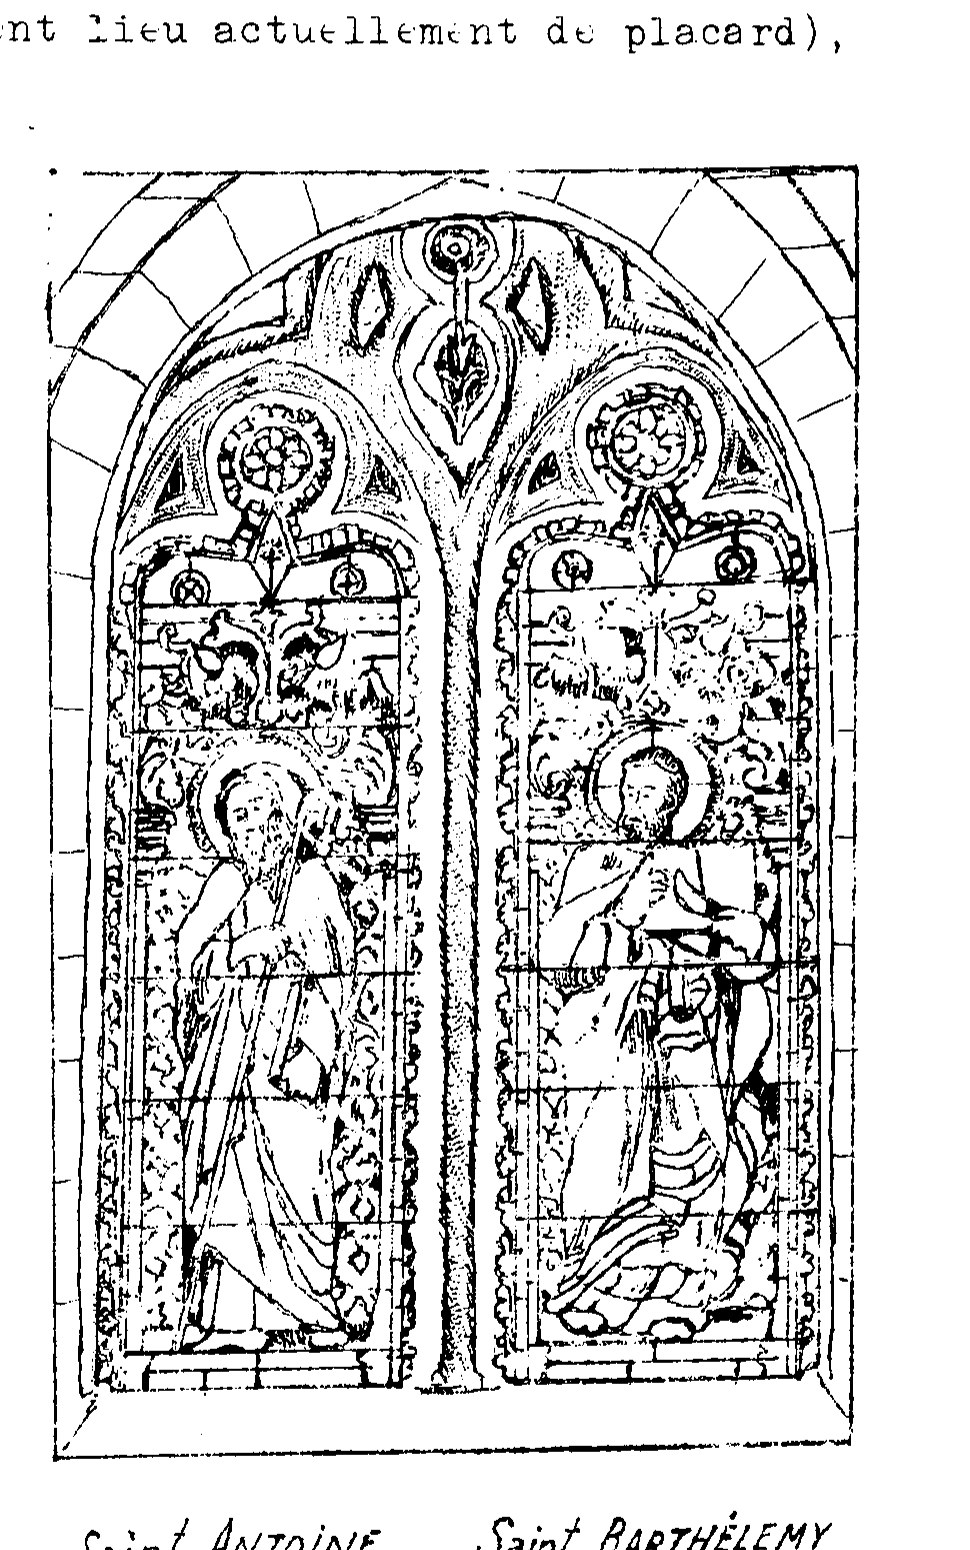
\includegraphics[width=0.62\textwidth]{Illustrations/illus-saint-antoine-barthelemy.jpg}\end{center}
% --- Page imprimée 218 — vue 221 (suite)
sculptés également par Mr Labrosse, ont été donnés par Mme Rambaud née Denise Berloty, à l'occasion de son mariage en 1874.

Cette même année Mr Bouteille remplaça le carrelage de l'église fait par Mr Pollocé en pierre du pays, par des dalles plus régulières sortant des carrières de Tramayes. Pour la chapelle de la Ste Vierge on a utilisé le dessus des anciens autels.

Ces diverses restaurations ont exigé une dépense considérable et la paroisse à elle seule eut été dans l'impossibilité d'y subvenir sans la générosité d'une famille généreuse et zélée qui venait de se fixer à Ouroux. Mr Berloty, nouveau propriétaire de Gros-Bois donna sans compter et Mr Bouteille ne fut point obligé, comme ses prédécesseurs de ne compter uniquement que sur les ressources, très modiques, de la Fabrique.

Aussi a-t-il doté notre paroisse d'une église ornée avec goût et même avec richesse.

Quelques années plus tard, Mr Aubert acheta un nouveau chemin de croix qui fut érigé en Juin 1894. Le prédicateur fut Mr le Chanoine Canard, missionnaire de la Maison des Chartreux, à Lyon.

\begin{center}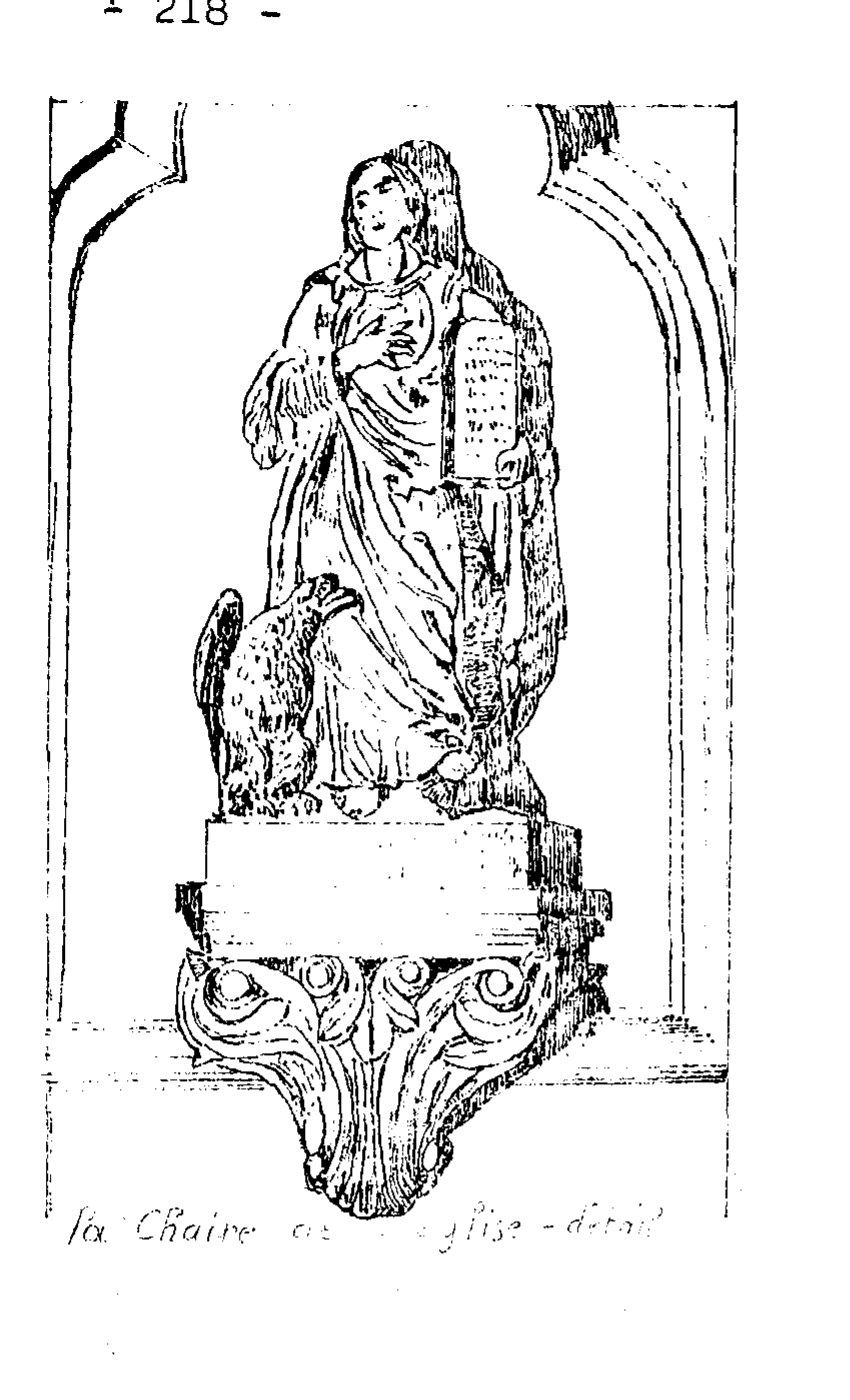
\includegraphics[width=0.62\textwidth]{Illustrations/illus-chaire-bois.jpg}\end{center}

\begin{center}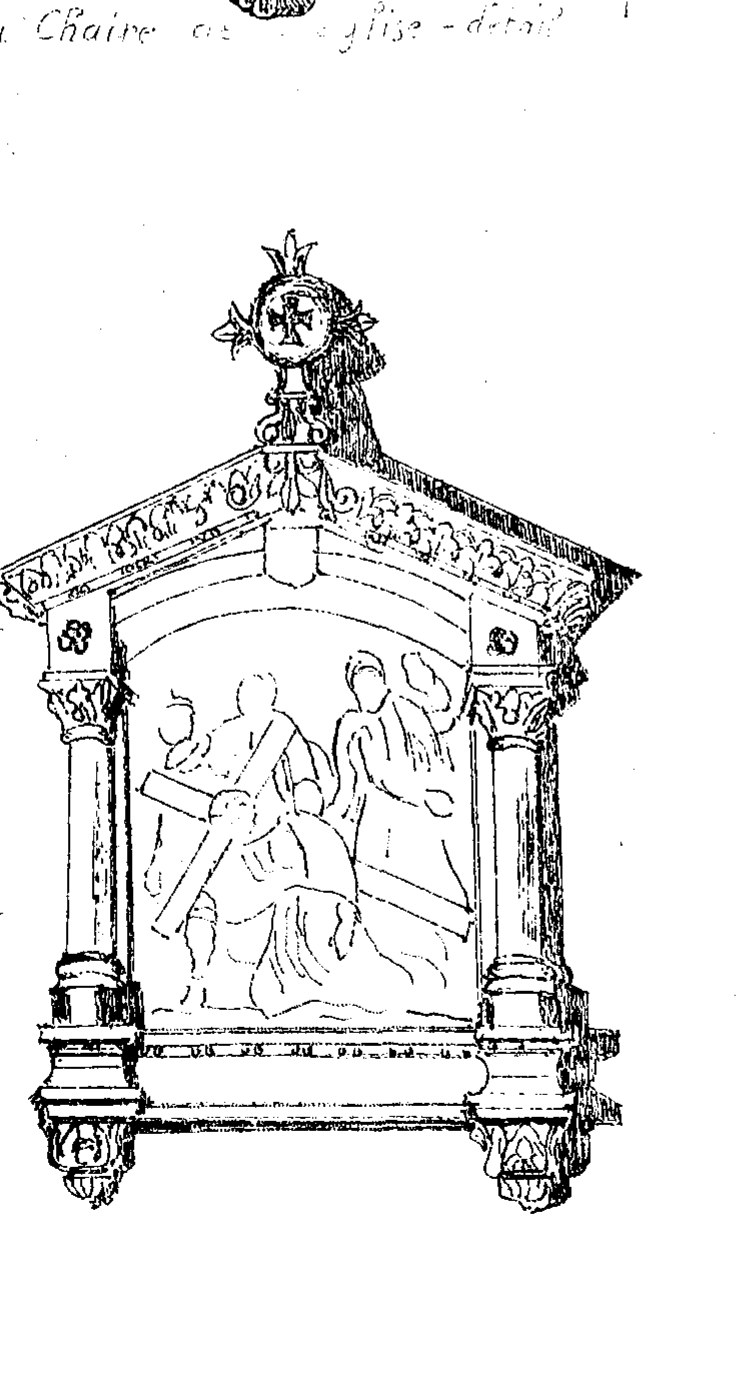
\includegraphics[width=0.62\textwidth]{Illustrations/illus-chaire-decor.jpg}\end{center}

% --- Page imprimée 219 — vue 222
Deux ans plus tôt, il avait fait réparer les autels de la Ste Vierge et de St-Antoine. Il confia les sculptures de ces deux chapelles à Mr Bourgeot qui travailla d'après les dessins de l'architecte du nom de Bresson. Les plâtres et les peintures furent retouchés. Deux grandes statues du Sacré-Cœur et de St-Joseph furent placées. La table de communion qui se trouvait alors plus près de l'autel fut déplacée vers la nef centrale. Elle avait été faite en 1779 par un nommé Bourgeot, serrurier à Villefranche. Par suite de son déplacement elle dut être agrandie. C'est Mr Benat, serrurier à Ouroux qui fit ce travail en 1900. La pierre qui se trouvait au centre de la table de communion et qui avançait un peu vers la nef centrale a été utilisée pour servir de balcon au-dessus de l'entrée de la salle des Fêtes.

En 1904 le curé Planus fit faire quelques réparations : Jean Claude Jandeau, menuisier à Ouroux fit le socle des Fonts baptismaux, Mr Montel, plâtrier peintre à Ouroux, aidé d'un habile ouvrier de Beaujeu, repeint le fond du chœur où se trouve la croix.

Les bancs de l'église ont été placés en 1905 par l'intermédiaire de Mr Berloty. C'est l'atelier de Mr l'Abbé Boisard de Lyon qui les a confectionnés. Ils ont coûté près de 4000 francs.

En 1909 des réparations urgentes sont à faire à la toiture de l'église. La toiture du clocher est particulièrement en très mauvais état et on signale des chutes de tuiles. Après plusieurs délibérations du Conseil municipal et l'approbation de la préfecture, les réparations de l'église sont données à Mr Gobet charpentier à Ouroux et Mr Laurent zingueur à Monsols.

Nous lisons dans le registre des délibérations du conseil à la date du 23 Juillet 1911, 10 h ½ : « Le Conseil à l'unanimité et en raison de la dépense qui résulterait de la réfection du clocheton de l'église, est d'avis de le démolir et fixe à 80 frs la somme à affecter à ce travail ». Présents : MM. Gonnet, Large, Champagnon A., Riboud, Gobet, Champagnon Ph., Prat et Canard, maire. Absents : MM. Triboulet, Voland, Chevalier, Rollet.

A-t-on eu raison ou tort de démolir ce clocheton qui donnait, à notre église un cachet particulier ? Certains ont affirmé que les
% --- Page imprimée 220 — vue 223 (suite)
frais de réparation du clocheton n'auraient guère été plus élevés que ceux occasionnés pour sa démolition. L'église, sans son ancien clocheton n'en demeure pas moins belle, mais n'empêche que tous les anciens qui ont connu leur église avec son ancienne parure ont beaucoup regretté cette disparition.

Un autre regret est celui de la disparition de l'ancienne horloge monumentale installée dans le clocheton. La petite cloche qui servait à la sonnerie des heures est actuellement fixée au plafond du clocher, au-dessus des trois grosses cloches. Le mécanisme de l'horloge placé à l'intérieur du clocher devenait de plus en plus hors d'usage. Pendant quelque temps on entendit encore sonner les heures, mais sans les voir, car aucun cadran extérieur n'avait été installé, puis un jour on n'entendit plus rien. La vieille horloge n'avait survécu que peu de temps au vieux clocheton. Actuellement, en 1952, de grosses réparations ont commencé à l'église. Il s'agit de la réparation de la toiture du clocher. Il est question, selon le désir de l'ensemble de la population, d'envisager l'installation d'une horloge monumentale, du moins de prévoir son emplacement. Mais la Commune d'Ouroux, ayant fait il y a quelques années une demande pour faire classer le clocher et le chœur de l'église comme monument historique, il faut consulter les Beaux Arts. De plus la lenteur de tout ce qui est « administratif », et la négligence de l'architecte communal qui laisse traîner les travaux ne nous donnent guère d'espoir.

En 1918, le Conseil décide de faire exécuter immédiatement les réparations urgentes de la charpente intérieure du clocher. En 1924 rien n'a encore été fait puisque nous lisons dans le registre des délibérations : « des réparations urgentes s'imposent à l'église, au clocher en particulier dont le mauvais état pourrait devenir un risque pour la circulation. »

En 1924, le 17 septembre, en voulant détruire par le feu un essaim d'abeilles qui logeait à l'intérieur de la boule qui entoure le pied de la croix, un ouvrier faillit provoquer un incendie qui, s'il n'avait été combattu à temps aurait pu ravager tout le clocher. Le conseil vote ensuite la répartition suivante :

% --- Page imprimée 221 — vue 224
\begin{center}
\begin{tabular}{@{}p{0.78\textwidth}r@{}}
frais de réparations du clocher (couvreur-zingueur) & 1148 frs \\
indemnité aux pompiers de Vaurenard & 100 \\
indemnité aux pompiers de Tramayes & 100 \\
indemnité à Mr Matray Joseph (transport pompe) & 50 \\
indemnité à Mr Benat Jean Louis & 25 \\
indemnité à Mr Jambon Jean Louis & 25 \\
note du charpentier (Montibert) & 241 \\
\multicolumn{2}{r}{1689 frs}
\end{tabular}
\end{center}

En 1925 le total des notes réglées s'élève à 1510 frs 75, et il est décidé que la note Chevalier sera réglée après réfection des travaux mal exécutés au clocher.

En 1930 la Commune fait réparer par Mr Bouillard, maçon, les deux escaliers de l'église.

En février 1939, Mr le Maire invita Mr le Préfet du Rhône, en déplacement dans le canton à l'occasion du conseil de revision tenu à Monsols, à venir visiter l'église. Mr le Préfet a répondu très aimablement à son appel. A la suite de cette visite Mr le Préfet écrivit au maire qu'il demanderait provisoirement l'inscription sur l'inventaire supplémentaire des monuments historiques du clocher et du chœur de l'église. Le conseil après avoir délibéré décida de remercier Mr le Préfet de cette proposition et de l'accepter en espérant qu'il n'y aura là qu'une étape intermédiaire et rapidement franchie avant d'avoir un classement définitif.

Voici quelques restaurations ou aménagements que Mr l'Abbé Delvaux, curé d'Ouroux de 1935 à 1944, a fait faire à notre église :

En 1936 les vitraux ont tous été resuivis et réparés. Tous les vitraux du chœur ont été doublés par les soins de Mr Nicolas Szekely, moyennant la somme de 3.800 frs. L'escalier qui conduisait au petit clocher a été supprimé en 1938. Une petite porte de sortie avec un escalier en pierre et ciment furent construits et permettent d'accéder à la sacristie de l'extérieur sans passer par l'église. L'ensemble de ces travaux a coûté 978 frs en 1939. En 1941 Mr Bachini, statuaire à Lyon, restaure les statues de St-Claude et de la Descente de croix, une statue représentant Notre-Dame de Lourdes fut achetée au prix de 1047 frs 90. Cette même année un grand harmonium est acheté. Il a coûté 4.800 frs. Notons encore l'électrification de diverses parties de l'église et l'installation d'un
% --- Page imprimée 222 — vue 225 (suite)
tambour vers la grande porte de l'église. Ce tambour, en chêne, a été exécuté par Mr Jandeau menuisier. Les pilastres et les moulures ont été fournis par les ateliers d'apprentissage de l'Abbé Boisard à Lyon. Les notes du menuisier, des ateliers d'apprentissage, du plâtrier (Mr H. Delrosso), du forgeron (Mr Mélinand) s'élèvent à la somme totale de 5385 frs 50 en l'année 1938.

Le successeur de Mr Velvaux, l'Abbé Magat fit faire plusieurs choses à l'église dont la principale fut la restauration des vitraux qui furent en partie détruits au cours du bombardement d'Ouroux, le 26 juillet 1944. Voici ce que nous lisons sur le constat fait par Mr A. Poinas, huissier à Monsols, le 20 octobre 1944 :

« …Me suis transporté à Ouroux et arrivé sur les lieux j'ai Antoine-Louis Poinas, huissier reçu au Tribunal Civil de Villefranche résidant à Monsols, soussigné, constaté ce qui suit :

« Le vitrail du chœur est endommagé sur 2 m2 environ

« Le vitrail grisaille du côté gauche en bois est complètement cassé, la surface est d'environ 2 m2 60

« Le vitrail grisaille du milieu est à refaire sur 3 m2 environ.

« Le vitrail représentant Ste Anne est endommagé et à refaire sur 2 m2 environ.

« Le vitrail grisaille de la chapelle de la Ste Vierge comporte un chassis ouvrant qui est cassé et une rosace peinte complètement endommagée.

« Le vitrail du côté droit de 2 m2 60 environ comporte trois panneaux cassés dont un ouvrant complètement démoli… »

Mr Magat s'adressa à la maison Jacqui de Lyon pour la réparation d'un vitrail grisaille du chœur, d'un autre du même genre du côté de la chapelle de la Sainte Vierge, ainsi que celui de Ste Anne. Les frais de ces diverses réparations se chiffrent à 13.170 frs. Quant aux quatre vitraux grisaille les plus près de la grande porte de l'église ils furent remplacés par quatre vitraux représentant St-Martin, St-Louis, Ste Bernadette et Ste-Jeannie d'Arc exécutés par la maison Lamy-Paillet de Lyon, d'après les dessins de l'artiste décorateur Luc Barbier. La facture de la maison Lamy-Paillet s'éleva à 146.405 frs, celle du décorateur à 16.000 frs. La paroisse d'Ouroux grâce aux dons reçus et au produit de diverses fêtes-Vermesses paya la somme élevée de 175.575 frs. Ajoutons à cette somme 57.491 pour le travail et les fournitures de trois artisans d'Ouroux que la Commune s'est chargée de payer avec l'argent reçu de la « Reconstruction ».

% --- Page imprimée 223 — vue 226
\begin{center}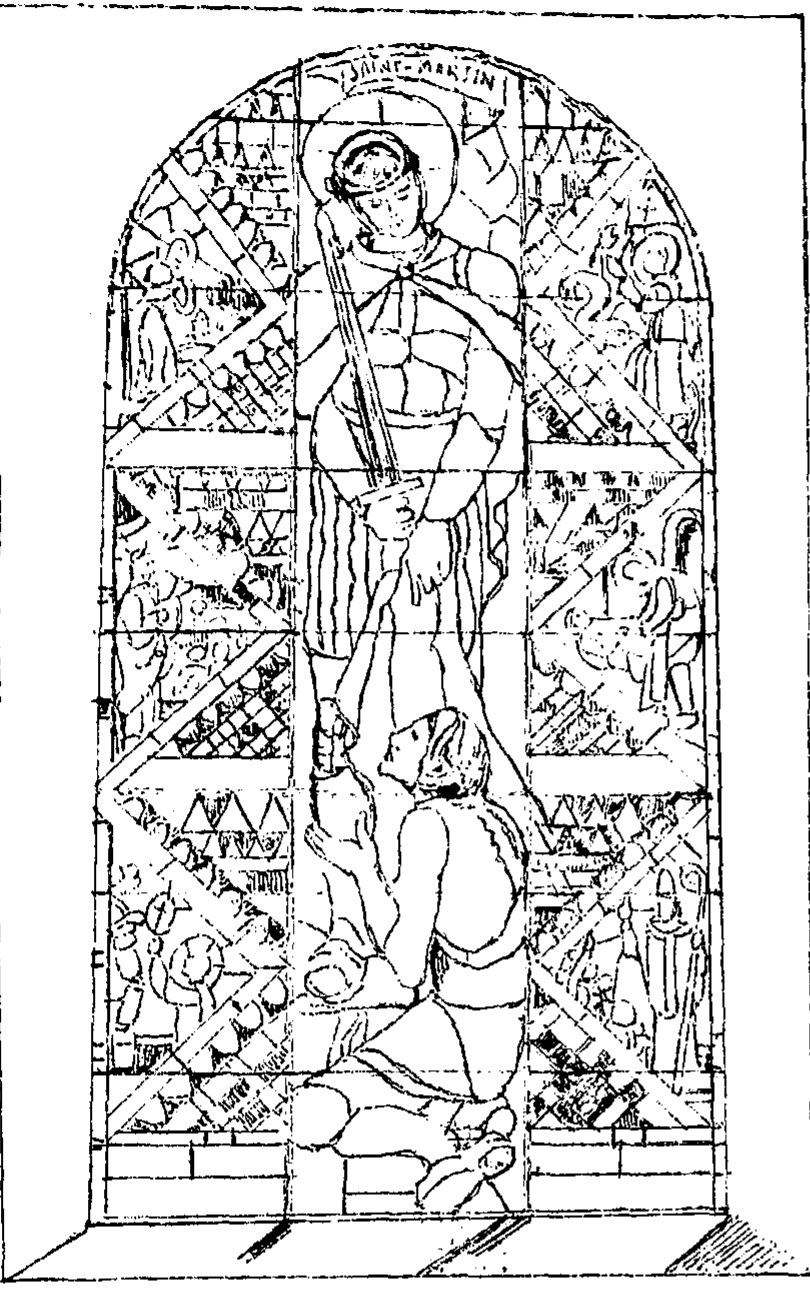
\includegraphics[width=0.62\textwidth]{Illustrations/illus-vitrail-saint-martin.jpg}\end{center}

\ourouxcaption{Vitrail de Saint-Martin}

Martin vivait au IVème siècle. Enrolé à 15 ans dans l'armée des Gaules, sa bravoure en fait vite un officier. Par un hiver vigoureux, Martin arrive aux portes d'Amiens. Un mendiant à peine vêtu grelotte sur le bord de la route. Martin s'arrête, coupe son manteau et en donne la moitié au pauvre (centre du vitrail).

À la fin de son engagement militaire, il entre dans les ordres. Revenu à Poitiers, il fonde le monastère de Ligugé, le premier monastère des Gaules (en haut et à gauche du vitrail). Martin s'adonne à la prédication (au milieu et à gauche). Martin détruit les idoles. À sa prière la foudre renverse une statue païenne (en bas et à gauche).

Martin avait refusé le sacerdoce par humilité. Il était simplement exorciste. Il est représenté chassant le démon symbolisé par un serpent qui vomit des flammes (vitrail en haut et à droite). Près de Paris, Martin embrasse un lépreux et le guérit. Un grand pin, objet d'un culte impie est abattu sur sa demande mais doit l'écraser en tombant. Il fait un signe de croix dans l'air, l'arbre se redresse pour s'abattre de l'autre côté. Pendant son absence un de ses catéchumènes meurt. Il prie des heures ; sa prière est exaucée et le mort ouvre les yeux et pourra être baptisé (vitrail au milieu et à droite). Les païens témoins de ses miracles se convertissent nombreux.

Enfin à la mort de l'évêque de Tours Martin, qui s'était enfermé à Ligugé est porté en triomphe jusqu'à Tours où il est malgré lui proclamé évêque (vitrail en bas et à droite). Saint Martin, apôtre des Gaules est un des saints les plus populaires de France.

% --- Page imprimée 224 — vue 227
\begin{center}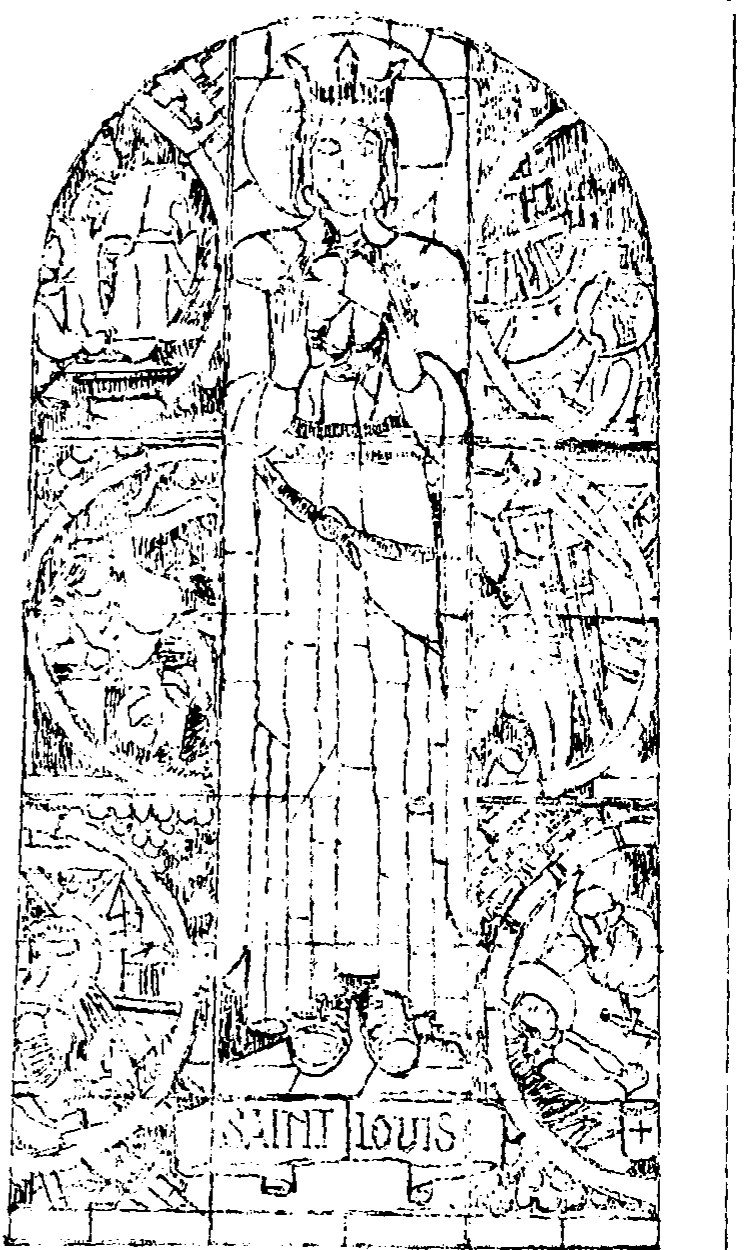
\includegraphics[width=0.62\textwidth]{Illustrations/illus-vitrail-saint-louis.jpg}\end{center}

\ourouxcaption{Vitrail de Saint-Louis}

Suivons de haut en bas les trois demi-médaillons de la partie gauche du vitrail. La première scène se passe à Poissy. St-Louis écrit. Son professeur est un moine. St-Louis aimera signer plus tard Louis de Poissy parce que baptisé à Poissy, près de Paris. La scène au-dessous se passe au bois de Vincennes. Saint Louis rend la justice sous un chêne. Au-dessous St-Louis est de passage à Ouroux. Il est un fait certain que Saint Louis s'est rendu à Cluny en 1248 avant de s'embarquer à Aigues-Mortes pour la croisade. Il a dû suivre la voie romaine qui traversait notre petit village et l'artiste s'est plu à rappeler le souvenir du passage à Ouroux du roi-chevalier.

En suivant le même ordre, nous voyons sur la droite du vitrail, en haut, St-Louis qui s'embarque à Aigues-Mortes pour l'Egypte en 1248 et pour Tunis en 1270. La scène suivante se passe à Mansourah, ville de la basse Egypte. On voit Saint Louis se défendant avec son épée, au cours d'un combat acharné. Il fut vaincu et fait prisonnier par les mameluks en 1250. La dernière scène représente la mort de St-Louis à Tunis (25 août 1270), où il s'était rendu espérant convertir le Sultan avant d'aller à Jérusalem. Son corps fut ramené à l'église de Saint-Denis près de Paris où l'on mettait les tombeaux de tous les rois de France. L'image centrale du vitrail représente St-Louis tenant respectueusement la couronne d'épines du Christ. L'une des plus grandes joies de St-Louis fut d'avoir pu acheter à l'empereur de Constantinople les reliques de la Passion. Pour abriter ces reliques il fit construire à Paris l'admirable Sainte-Chapelle.

% --- Page imprimée 225 — vue 228
\begin{center}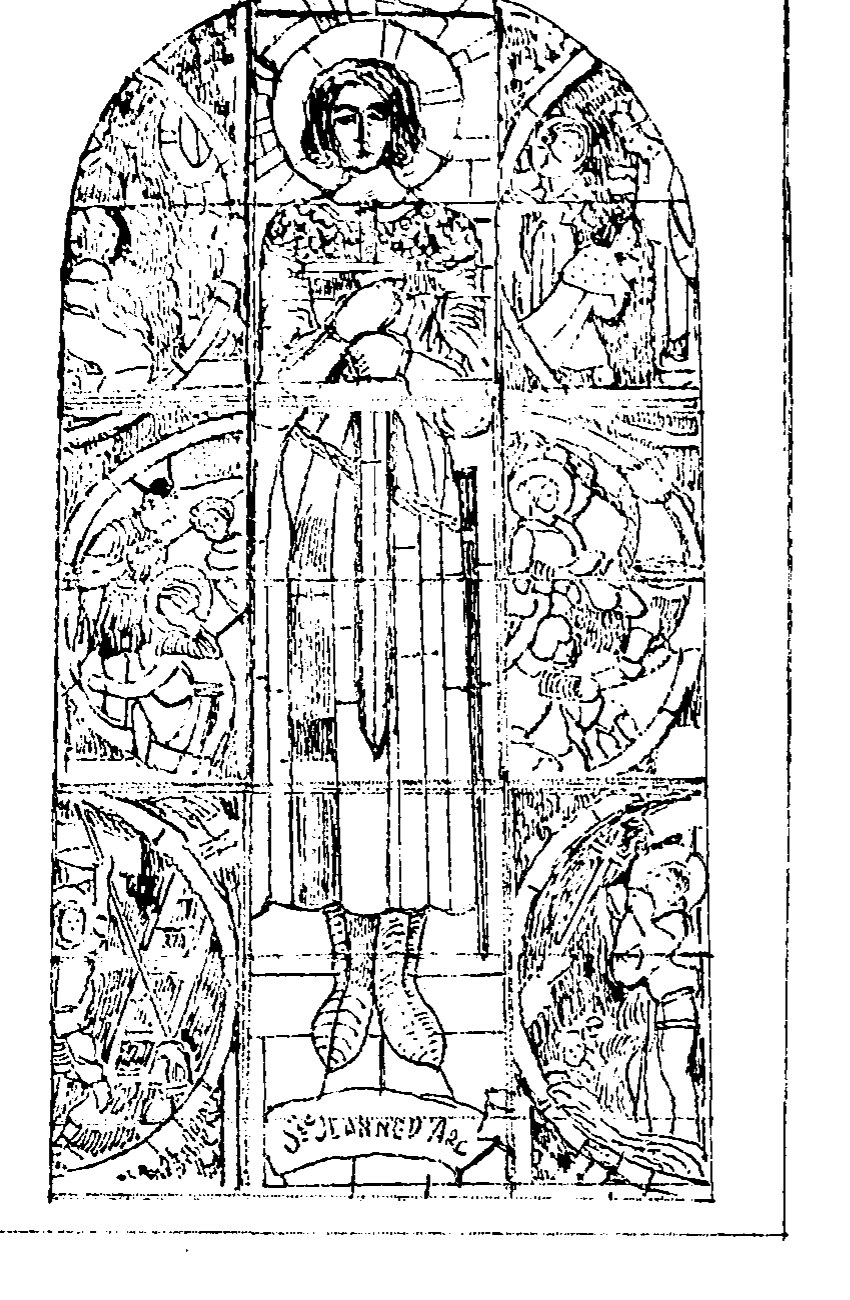
\includegraphics[width=0.62\textwidth]{Illustrations/illus-vitrail-jeanne-arc.jpg}\end{center}

\ourouxcaption{Vitrail de Sainte-Jeanne d'Arc}

Le sujet principal de ce vitrail représente l'héroïne qui sauva notre pays de France. Jeanne a su, en un temps de haine, de division, de perdition de la France, faire l'unité de la France, faire revivre la France, faire s'épanouir l'âme française. Cela a été le grand miracle de Jeanne. Puisque Jeanne a l'honneur d'être sur les autels nous pouvons souvent répéter les paroles que l'artiste a gravées à ses pieds : « Ste-Jeanne d'Arc priez pour le Salut de la France ». L'artiste a représenté Jeanne d'Arc avec une épée, car elle s'est faite guerrière, elle a commandé les hommes d'armes mais jamais elle ne s'est servie de son épée tellement elle avait horreur de voir couler le sang.

Les différentes scènes représentées sur les côtés du vitrail évoquent les grandes dates de la vie de Jeanne. C'est tout d'abord à Domrémy ; son petit village natal où Jeanne, à genoux, entend les voix des saints qu'elle vénérait : l'Archange St-Michel, Ste Marguerite et Ste Catherine. Puis elle s'en va trouver le roi Charles VII qui siégeait à Bourges et à Poitiers. À Orléans Jeanne est blessée d'une flèche mais elle est victorieuse et délivre la ville. Nous retrouvons Jeanne assistant au sacre de Charles VII à Reims où elle l'avait pressé d'aller. L'image suivante nous montre Jeanne cernée par les ennemis, jetée à bas de cheval et faite prisonnière à Compiègne. La scène finale nous montre Jeanne sur le bûcher à Orléans. Elle prie, elle demande la croix pour l'embrasser longuement. En trépassant elle cria à haute voix : « Jésus, Jésus ». Ce fut son dernier mot. Jeanne d'Arc était âgée de 19 ans quand elle mourut pour la France.

% --- Page imprimée 226 — vue 229
\begin{center}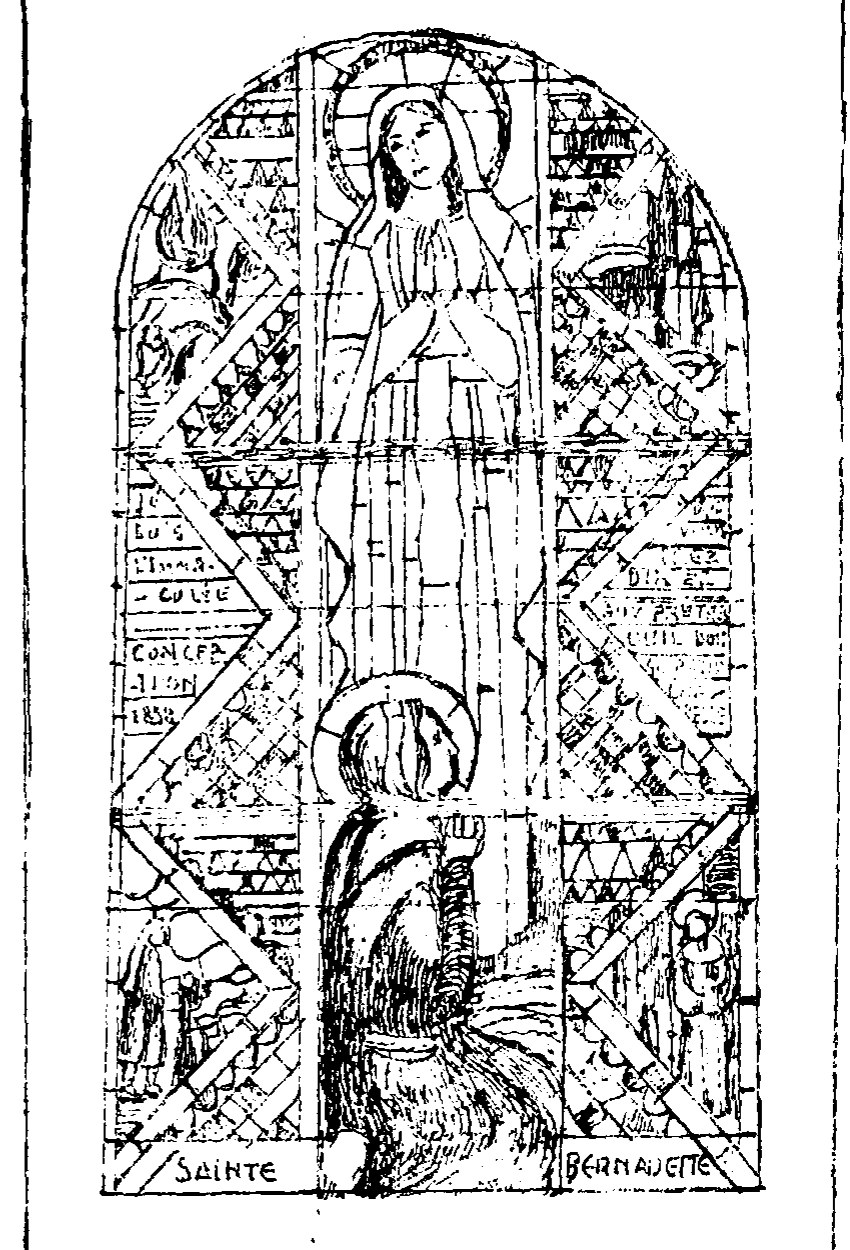
\includegraphics[width=0.62\textwidth]{Illustrations/illus-vitrail-bernadette.jpg}\end{center}

\ourouxcaption{Vitrail de Sainte Bernadette}

La grande image de ce vitrail rappelle l'apparition de la Vierge à Bernadette, à Lourdes. Bernadette est en prière aux pieds de la Vierge Immaculée.

Le 11 février 1858 trois jeunes filles allaient chercher du bois mort dans un ravin des Pyrénées. L'une d'elles s'appelait Bernadette Soubirous. Au moment où Bernadette allait traverser le torrent elle voit soudain une belle jeune fille dans l'anfractuosité de la roche de Massabielle. « Qui êtes-vous Madame ? » L'apparition sourit mais ne dit pas son nom. 18 fois Bernadette la reverra. La Sainte Vierge, car c'est elle, se nommera : « Je suis l'Immaculée Conception ». La Vierge lui demande de dire son chapelet. Et Bernadette voit « la Dame » faire glisser elle-même entre ses doigts les grains d'un rosaire qui pendait à son bras. Elle répète : « Pénitence, pénitence, pénitence pour les pécheurs ». Elle ajoute encore : « Vous irez dire aux prêtres qu'il doit se bâtir ici une chapelle ».

Les quatre dessins qui se trouvent aux angles du vitrail représentent Bernadette bergère, Bernadette puisant de l'eau au pied de la grotte, la chapelle qui fut bâtie, Bernadette religieuse à Nevers.

Et depuis ce temps Lourdes peut s'appeler la terre des miracles, tant les faveurs accordées par Marie sont nombreuses. On y vient de tous les pays du monde. C'est par centaines de milliers que les pèlerins viennent à Lourdes. Et la Vierge seule sait le nombre de ceux qui s'en retournent guéris, du corps pour quelques-uns, de l'âme pour un bien plus grand nombre.

% --- Page imprimée 227 — vue 230
Signalons maintenant toutes les dernières transformations ou aménagements faits à l'église, jusqu'à nos jours.

Mr le Curé Aubonnet, dès l'année de son arrivée, acheta un premier calorifère fonctionnant à la sciure, puis un second l'année suivante ; ce genre de chauffage n'oblige pas à une surveillance aussi fréquente que celui fonctionnant au bois et surtout est bien plus économique que le bois et le charbon. Les deux calorifères ont coûté au total 55.000 francs. La sciure qui est donnée gratuitement à tout preneur est prise, suivant les commodités, à l'une ou l'autre des quatre scieries GONNET, VOLAND au bourg, MATRAY au Frazay et JACQUET à Sauzay. Des deux anciens calorifères, l'un a été vendu à la paroisse de Poule, l'autre a été placé à la cure d'Ouroux.

En 1951 de nouveaux Fonts Baptismaux furent installés à l'église tout près des anciens dont la cuve était pratiquement inutilisable, mais dont la boiserie qui l'entoure (cf page 217) sert actuellement de placard pour retirer les objets servant aux Baptêmes. Ces nouveaux fonts baptismaux ont été commandés à la maison Bachini de Lyon. Ils ont été taillés dans des blocs de pierre de St-Martin. Les pantures de bronze qui embellissent le couvercle en chêne massif ont été données gratuitement par Mr CHUZEL, bronzier à Lyon et ami de Mr le curé. Ces Fonts-Baptismaux aux lignes sobres et belles s'harmonisent tout-à-fait avec le style de l'église. Une barrière en fonte, achetée d'occasion, peinte en imitation bronze clôture admirablement cette petite chapelle des Fonts baptismaux.

\begin{center}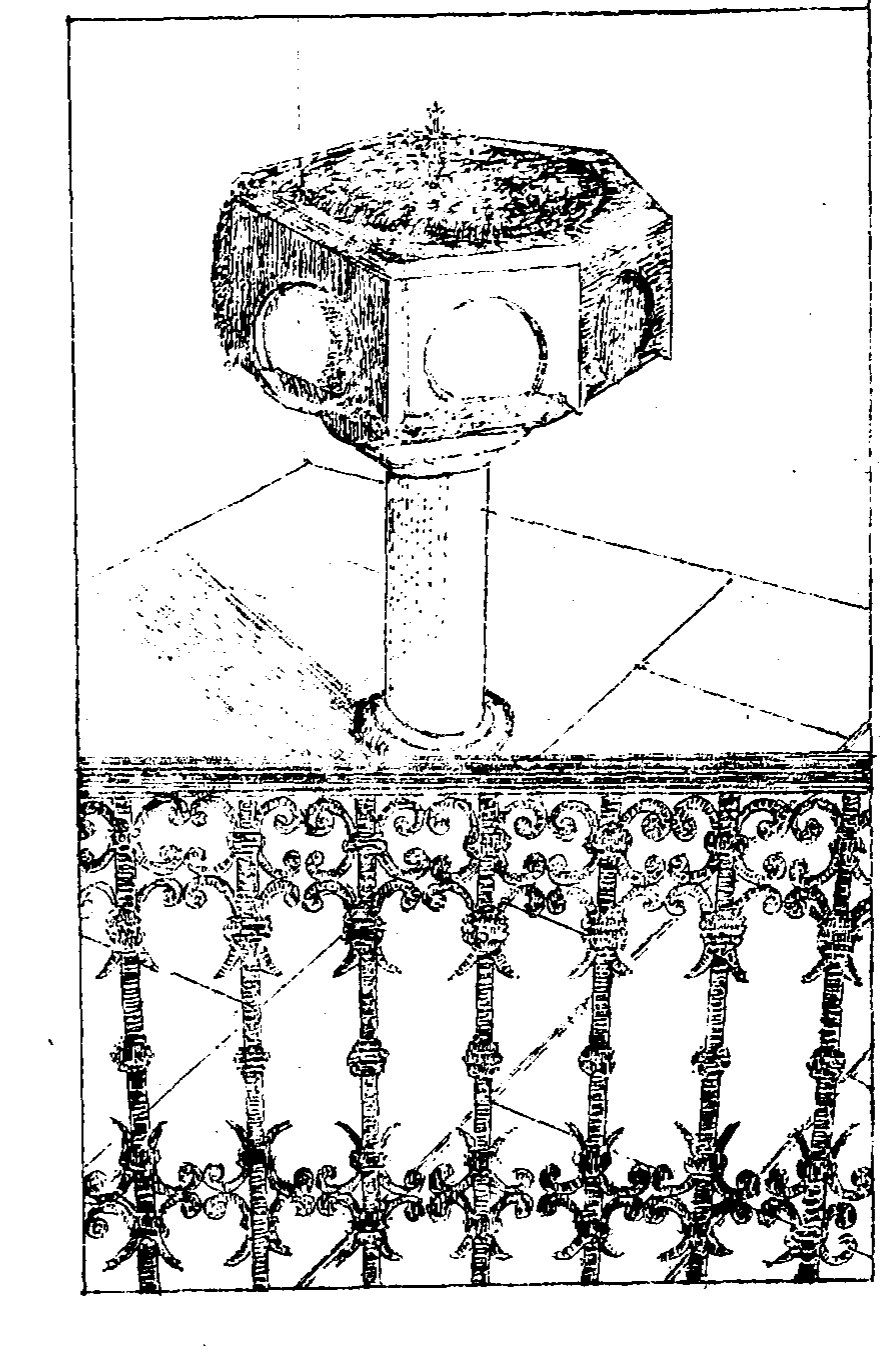
\includegraphics[width=0.62\textwidth]{Illustrations/illus-fonts-baptismaux.jpg}\end{center}

% --- Page imprimée 228 — vue 231
Baptismaux. (voir plan de l'église à la page 204). Le prix de revient s'élève à un total de 126.500 francs. En voici d'ailleurs le détail :

Fonts Baptismaux en pierre St-Martin : 72.000 frs ; barrière d'occasion remise à neuf : 37.500 frs ; transport et pose : 7.500 frs ; dallage du sol, bouchage d'une porte et crépissage d'un morceau de mur : 9.500 francs.

La somme nécessaire pour payer ces dépenses a été trouvée grâce aux quêtes faites à l'église et à quelques dons de généreux paroissiens.

Vers la fin de l'année 1952, avant la fête de Noël, une autre petite transformation eut lieu à l'intérieur de l'église. Tous les chandeliers de cuivre furent diminués de hauteur et redorés. Les souches électriques furent remplacées par d'autres plus courtes. Sans vouloir remplacer les très hauts chandeliers que possédait notre église par d'autres plus modernes mais très bas et pas toujours appréciés de tous, on se contenta de faire modifier quelque peu ce que la paroisse possédait. Ce travail fut exécuté avec goût par la maison CHUZEL de Lyon. Les deux jeux de chandeliers du maître-autel ont été mis à hauteur du tabernacle en les réduisant de 10 centimètres. Les chandeliers des autels de la Ste Vierge et de St-Antoine furent diminués d'une manière plus sensible, presque de moitié. Mais là encore, plus qu'au maître-autel cela était nécessaire pour dégager et mettre en relief les sculptures et inscriptions des deux autels secondaires qui étaient plus ou moins masqués par des chandeliers bien trop hauts. Signalons que la belle garniture de chandeliers romains du maître-autel (celle que l'on met pour les grandes fêtes) a coûté en mai 1875, 570 francs. Elle est estimée en 1952 au prix de 140.000 francs.

Quels sont les travaux à envisager dans un avenir prochain ?

Tout d'abord, dès le retour des beaux jours ce sera la finition de la couverture du clocher. Actuellement (en décembre 1952) la croix en fer a été redressée et repeinte, le coq a été redoré. Il est presque certain que les couvreurs ne referont pas les dessins qui, de loin, se remarquaient sur les pans du toit, tel cet ostensoir qui faisait désigner notre église de la part des étrangers par ces mots : « l'église à l'ostensoir ». Ce ne seront là que des vieux souvenirs qui disparaîtront avec le temps.

% --- Page imprimée 229 — vue 232
\begin{center}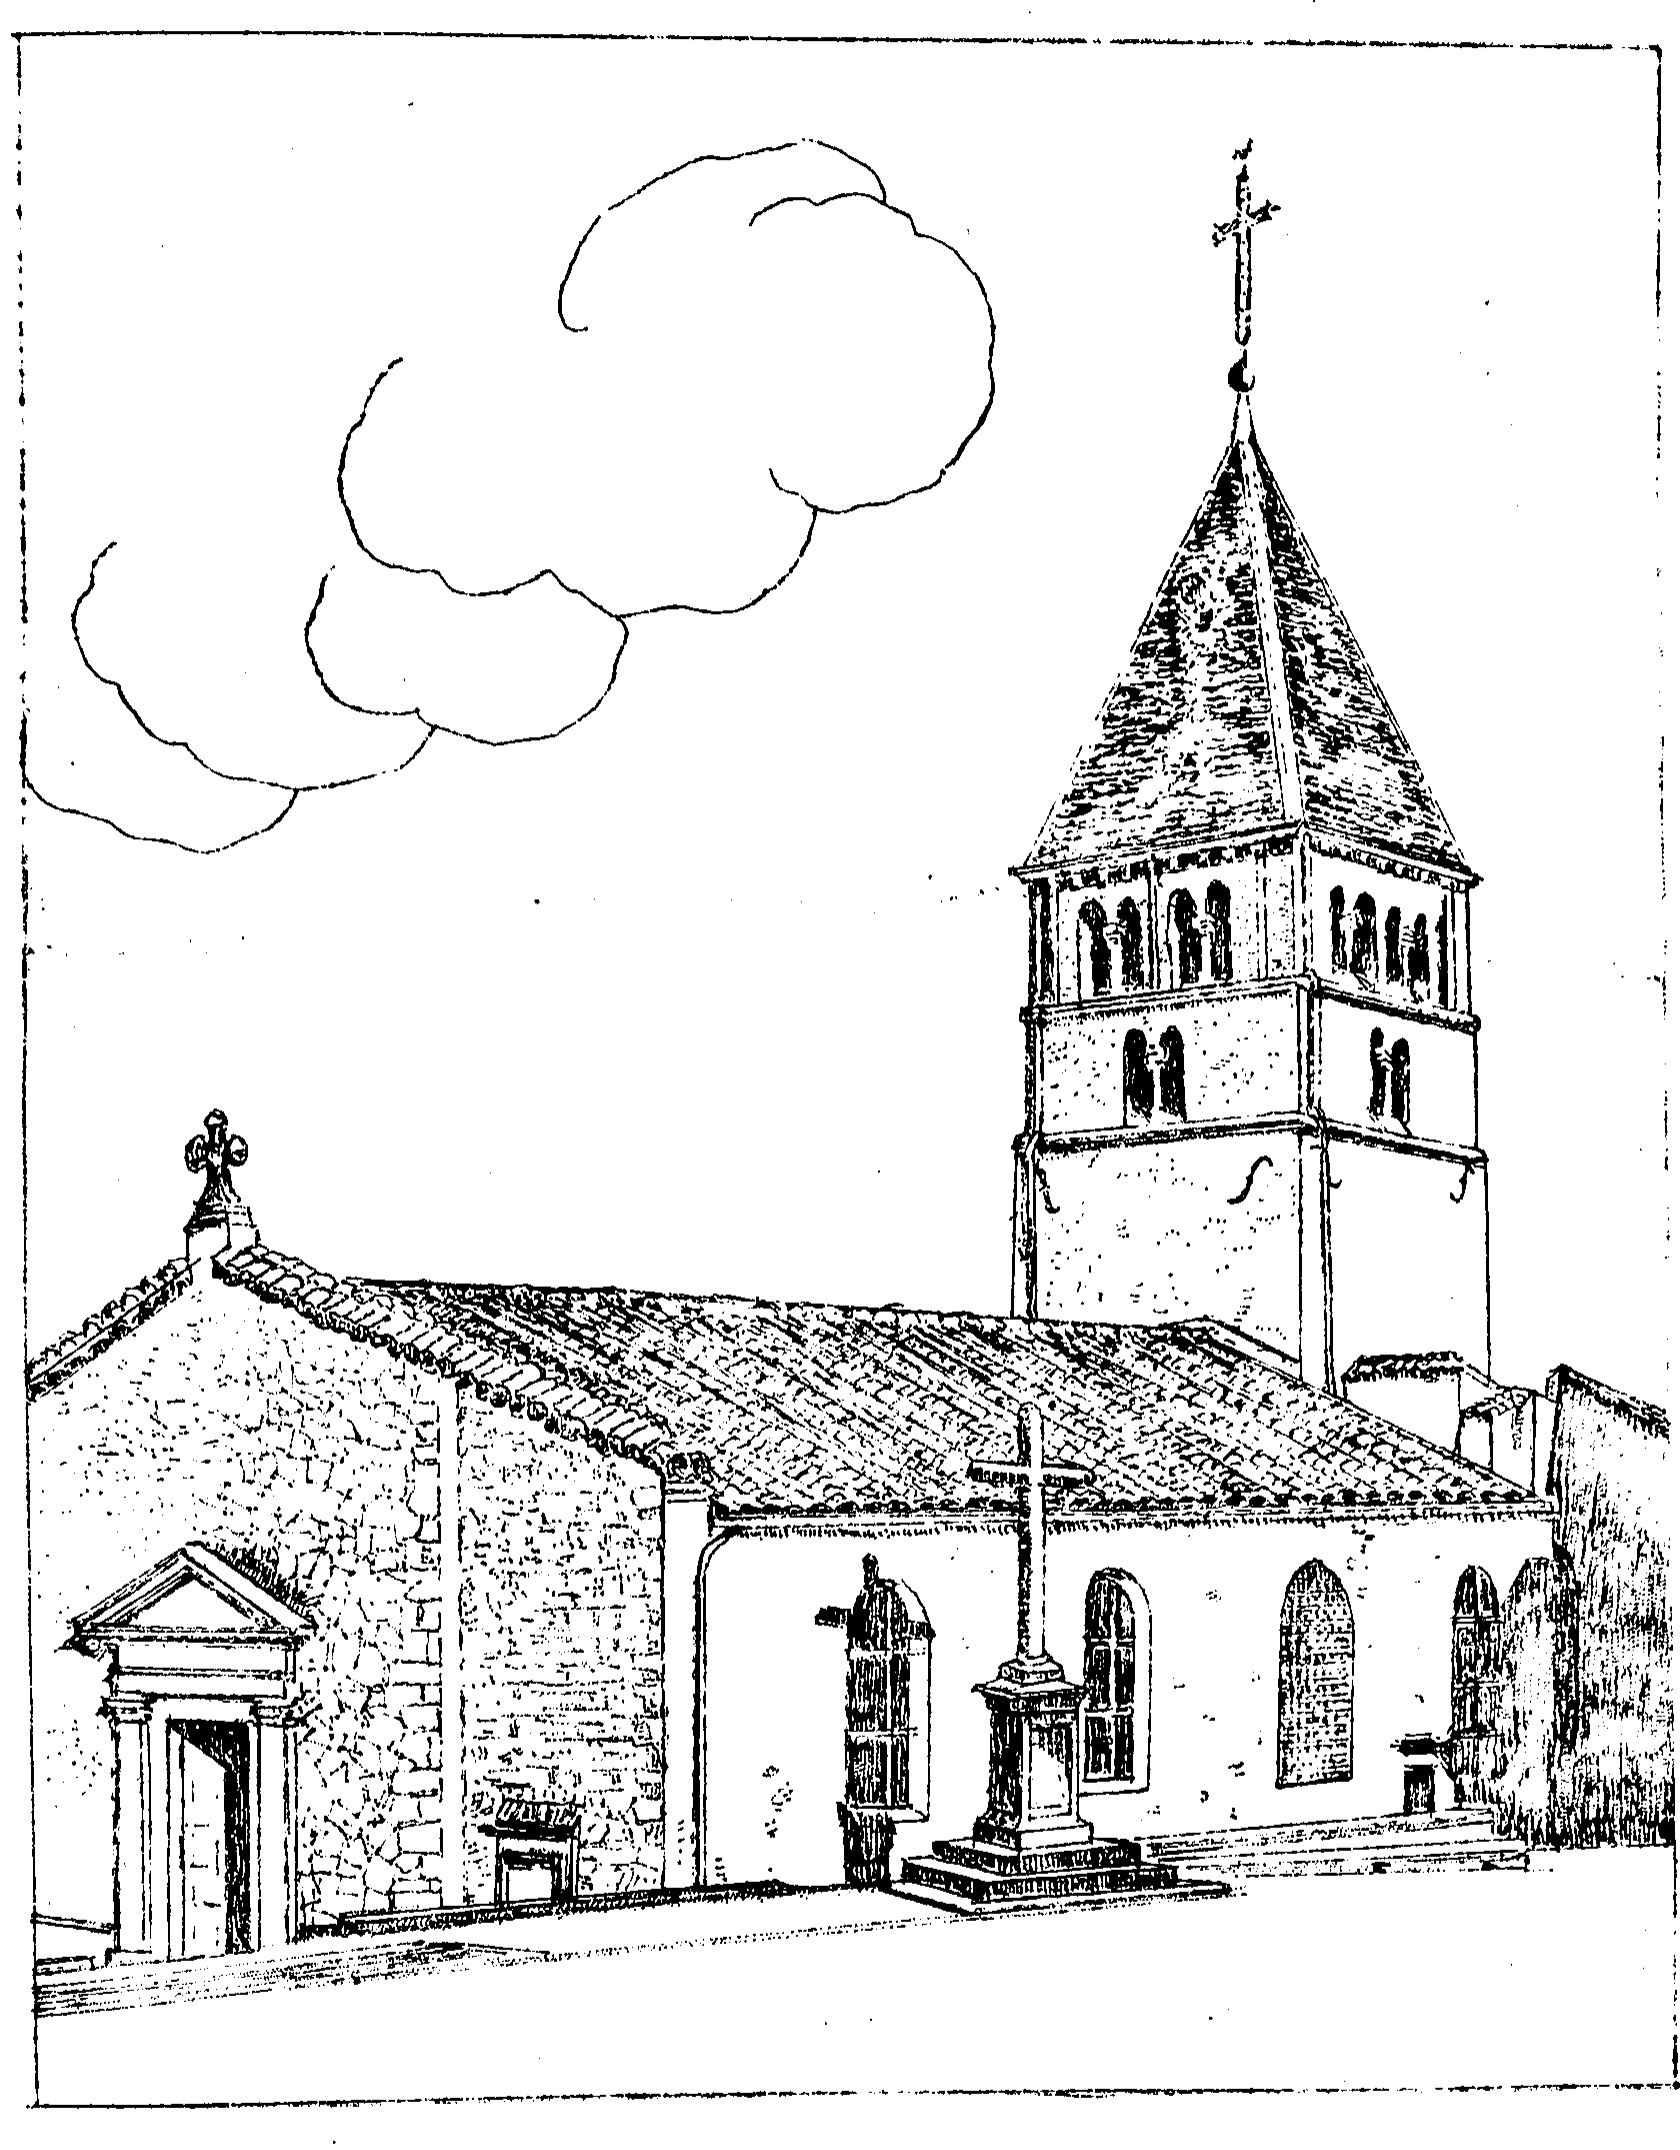
\includegraphics[width=0.62\textwidth]{Illustrations/illus-eglise-final.jpg}\end{center}

% --- Page imprimée 230 — vue 233
Une fois les travaux du clocher terminés, la Commune doit faire refaire les plafonds de l'église dont les plâtres à quelques endroits ont été quelque peu endommagés par le bombardement de 1944.

Il y aura lieu ensuite de faire restaurer tous les badigeons des murs intérieurs. Cela sera à la charge de la Paroisse. Les six colonnes de l'église que surmontent d'intéressants chapiteaux historiés gagneraient en beauté d'être dépouillées de leur couche de peinture sombre et de retrouver la teinte naturelle de ses pierres de taille. Il y aurait également intérêt, un jour ou l'autre, à remplacer les deux énormes statues en plâtre représentant St-Joseph et le Sacré Cœur placées de chaque côté de la table de communion, par deux autres représentant les mêmes personnages, mais qui soient dans une proportion moins choquante avec les autres statues de l'église.

Enfin un dernier souhait, déjà signalé plus haut. Souhaitons qu'une municipalité avisée et dynamique trouve une solution pour faire placer dans un jour très prochain une horloge au clocher. Il y a certainement à tout problème, même compliqué qu'il paraisse, une solution possible. Une chose comme celle-ci intéresse tous les habitants d'une commune et d'une paroisse. Aussi l'une et l'autre pourraient mener à bien un tel projet qui à l'heure actuelle, dans notre localité, germe dans tous les esprits.

Le Saint Curé d'Ars, dont tout le monde connaît l'esprit de pauvreté et de pénitence, trouvait que rien n'était trop beau ou trop riche pour son église. Que ne ferait-on en effet pour la maison de Dieu !

C'est la maison dans laquelle sont consacrés les grands moments de notre vie chrétienne : la naissance par le Baptême, l'adolescence par la Communion, la jeunesse par le Mariage. C'est aussi le lieu où chaque Dimanche les enfants de Dieu se rencontrent avec leur Père du ciel et où avant d'être porté en terre notre corps est une dernière fois conduit. Voilà pourquoi nous devons être fiers de notre église, voilà pourquoi nous devons aussi l'aimer et travailler sans cesse à la conserver très belle malgré ses vieux ans !
